\documentclass[aspectratio=169,xcolor=table]{beamer}
\usepackage{epstopdf}
\usepackage{textgreek}
\usepackage{physics}
\usepackage{appendixnumberbeamer}
\usepackage{multicol}
\usepackage{pbox}
\usepackage{amssymb}
\usepackage{xcolor}
\usepackage{blindtext}
\usepackage{color, colortbl}
\usepackage{xspace}
\usepackage{listings}
\usepackage{tikz}
\usetheme{NIU}

% suppress navigation bar
\beamertemplatenavigationsymbolsempty

% Title
\title[2022 PhD Progress Review]
{2022 PhD Progress Review}

% Sub Title
% \subtitle{Sub Title}

% Author
\author[Elliot Parrish]
{\texorpdfstring{\underline{Elliot Parrish}}{Elliot Parrish}\inst{\dag} \and Dhiman Chakraborty\inst{\dag} \and Jahred Adelman\inst{\dag}}
\hypersetup{pdfauthor={Elliot Parrish}}

% - Give the names in the same order as the appear in the paper.
% - Use \and to separate authors name
% - Use the \inst{?} command only if the authors have different affiliation.

\institute[NIU] {\inst{\dag}Northern Illinois University, USA}
% \institute[IFJ PAN] {}
% - Use the \inst command only if there are several affiliations.
% - Keep it simple, no one is interested in your street address.

\date{January 20, 2022}
% \subject{} % only for pdf info

% if you want to disable section, subsection title page display, uncomment accordingly 
\AtBeginSection[]{
  \begin{frame}
  \vfill
  \centering
  \begin{beamercolorbox}[sep=8pt,center,shadow=true,rounded=true]{title}
    \usebeamerfont{title}\insertsectionhead\par%
  \end{beamercolorbox}
  \vfill
  \end{frame}
}
\AtBeginSubsection{}

% Title Graphics add befor titlepage
\titlegraphic{\includegraphics[height=2.5cm]{NIU_logo.eps}}

\newcommand{\specialcell}[2][l]{%
  \begin{tabular}[#1]{@{}l@{}}#2\end{tabular}}

\newcommand{\Cross}{$\mathbin{\tikz [x=1.4ex,y=1.4ex,line width=.2ex, red] \draw (0,0) -- (1,1) (0,1) -- (1,0);}$}%
\newcommand{\Hp}{\ensuremath{H^{\pm}}\xspace}
\newcommand{\Etm}{\ensuremath{E_\text{T}^\text{miss}}\xspace}
\newcommand{\pt}{\ensuremath{p_\text{T}}\xspace}
\newcommand{\HpLong}{\ensuremath{\Hp \rightarrow \tau \nu}\xspace}

\begin{document}
\frame{\titlepage}

% add logo after title page, so it does show on title page
\logo{\includegraphics[trim=1cm 2.5cm 1cm 0,clip,width=1.3cm,keepaspectratio=true]{NIU_logo.eps}}
% \logo{\includegaraphics}


% Table of Contents
% \begin{frame}<beamer>{Table of Contents}
%     \tableofcontents
% \end{frame}

\begin{frame}{\contentsname}
  \begin{multicols}{2}
    \tableofcontents
  \end{multicols}
\end{frame}

\section{Timeline }

  \begin{frame}[t]{Timeline to 2022}
    \begin{columns}
      \column[t]{.5\linewidth}
        \begin{itemize}
          \item \textbf{Summer 2017:}  {\footnotesize{@ NIU
            \begin{itemize}
              \item Started at NIU
              \item Started ATLAS qualification task on the hadronic Tile calorimeter
            \end{itemize}}}

          \item \textbf{Summer 2018: } {\footnotesize{@ CERN
            \begin{itemize}
              \item Qualified as author on ATLAS
              \item Start training as Tile Calorimeter Data Quality (DQ) Co-Coordinator 
              \item Tile test beams
              \item \href{https://indico.cern.ch/event/687473/}{\textcolor{blue}{\emph{Machine Learning for High Energy Physics Summer School}}}
              \begin{itemize}
                \item University of Oxford
                \item August 6, 2018 - August 12, 2018
              \end{itemize}
            \end{itemize}}}

        \end{itemize}

      \column[t]{.5\linewidth}
        \begin{itemize}
          \item \textbf{Fall 2018: } {\footnotesize{@ NIU
            \begin{itemize}
              \item Take over full time as DQ Co-Coordinator
              \item Finished collecting Run-2 data
            \end{itemize}}}

          \item \textbf{Summer/Fall 2019: } {\footnotesize{@ CERN
            \begin{itemize}
              \item Ramped up work on \HpLong analysis
              \item ATLAS data quality \href{https://arxiv.org/abs/1911.04632}{\textcolor{blue}{Run-2 paper}}
              \item Reprocessing campaign of Run-2 data starting
              \item Moved to CERN long term
            \end{itemize}}}

        \end{itemize}

    \end{columns}
  \end{frame}

  \begin{frame}[t]{Timeline to 2022}
    \begin{columns}
      \column[t]{.5\linewidth}
        \begin{itemize}

          \item \textbf{Spring 2020: } {\footnotesize{@ CERN
            \begin{itemize}
              \item Polish National Agency for Academic Exchange: \emph{International Scholarship Exchange of PhD Students and Academics}
                \begin{itemize}
                  \item February 17, 2020 - February 2021, 2020
                  \item Institute of Nuclear Physics Polish Academy of Sciences, Krakow, Poland
                \end{itemize}
            \end{itemize}}}


          \item \textbf{Summer 2020: } {\footnotesize{@ CERN
            \begin{itemize}
              \item On detector readout and control electronics maintenance
              \item Started \HpLong PNN HPO
            \end{itemize}}}

        \end{itemize}

      \column[t]{.5\linewidth}
        \begin{itemize}

          \item \textbf{Fall 2020: } {\footnotesize{@ CERN
            \begin{itemize}
              \item Reprocessing monitoring tests
            \end{itemize}}}

          \item \textbf{Spring/Summer 2021: } {\footnotesize{ @ CERN
            \begin{itemize}
              \item Tile ACES (equipment inventory)
              \item Trained replacement DQ Co-Coordinator
              \item Finalized Run-2 reprocessing preparations
              \item APS \href{https://indico.cern.ch/event/1034469/contributions/4427261/}{\textcolor{blue}{DPF 2021}}
            \end{itemize}}}

          \item \textbf{Fall 2021: } {\footnotesize{@ USA
            \begin{itemize}
              \item Tile test beams
              \item Moved from CERN back to US
              \item Finished involvement with Tile
              \item Switched to full-time \HpLong work
            \end{itemize}}}


        \end{itemize}

    \end{columns}
  \end{frame}
    
\section{Tile Calorimeter }

  \begin{frame}[t]{ATLAS Hadronic Tile Calorimeter}
    \begin{columns}
      \column{.6\textwidth}
        \begin{itemize}
          \item ATLAS is a general purpose particle detector on the Large Hadron Collider at CERN
          \item The Hadronic Tile calorimeter is the outermost sub-detector besides the muon system
          \begin{itemize}
            \item Designed to measure hadron energy by fully absorbing particle showers
            \item Highly important in jet reconstruction
            \item Scintillating tile with steel absorber
            \item Light readout via optical fibers to PMTs
          \end{itemize}
        \end{itemize}
        \centering
        \includegraphics[height=.15\textheight,keepaspectratio=true]{LHC.png}
        \includegraphics[height=.25\textheight,keepaspectratio=true]{ATLASCrossSectionDiagram.png}

      \column{.4\textwidth}
      \centering
        \includegraphics[height=.4\textheight,keepaspectratio=true]{TileCalDiagramATLAS.png}
        \includegraphics[height=.4\textheight,keepaspectratio=true]{TileModuleCrossSection.png}

    \end{columns}
  \end{frame}

  \subsection{Authorship Task}

    \begin{frame}[t]{Tile Calorimeter Calibration Systems}
      \begin{columns}
      \column{.6\linewidth}
        \begin{itemize}
          \item Cesium
          \begin{itemize}
            \item Hydraulically moved throughout detector
            \item Measures response of scintillator
          \end{itemize}
          \item Laser
          \begin{itemize}
            \item Measures response of photomultiplier tubes
            \item Can be taken during physics data taking and individual calibration runs
          \end{itemize}
          \item Charge Injection
          \begin{itemize}
            \item Four capacitors, two low gain, two high gain
            \item Measures response of digitizers and readout electronics
          \end{itemize}
          \item One centralized database to store all calibration constants
        \end{itemize}
      \column{.4\linewidth}
      \centering
      \includegraphics[width=\textwidth,keepaspectratio=true]{Tile_Calibration_Diagram.png}
      \end{columns}
    \end{frame}

    \begin{frame}[t]{Centralized ATLAS Conditions Database}
      \begin{columns}
      \column{.45\textwidth}
        \begin{itemize}
          % \item Centralized database for all ATLAS subsystems
          % \begin{itemize}
            \item Online and Offline database
            \item Three main tags within databases
          % \end{itemize}
          \begin{itemize}
            \item UPD1
            \begin{itemize}
              \item Used to quickly process 10\% of events
              \item Can only append information
            \end{itemize}
            \item UPD4
            \begin{itemize}
              \item Used after 48 hrs to process full run
              \item Can change previous information
            \end{itemize}
            \item ONL01
            \begin{itemize}
              \item Online database used at Point 1
              \item Used for triggering
            \end{itemize}
          \end{itemize}
        \end{itemize}

        \column{.55\textwidth}
        \begin{itemize}
          \item TileCal Robot Authorship Task
          \begin{itemize}
            \item Web based interface to update conditions database (Tile internal)
            \item Previously, had to update all three tags individually
            \item Created automated syncing of tags
            % \begin{itemize}
            %   \item Channel status flags
            %   \item Timing calibration constants
            %   \item Cell noise
            % \end{itemize}
          \end{itemize}
        \end{itemize}
        \centering
        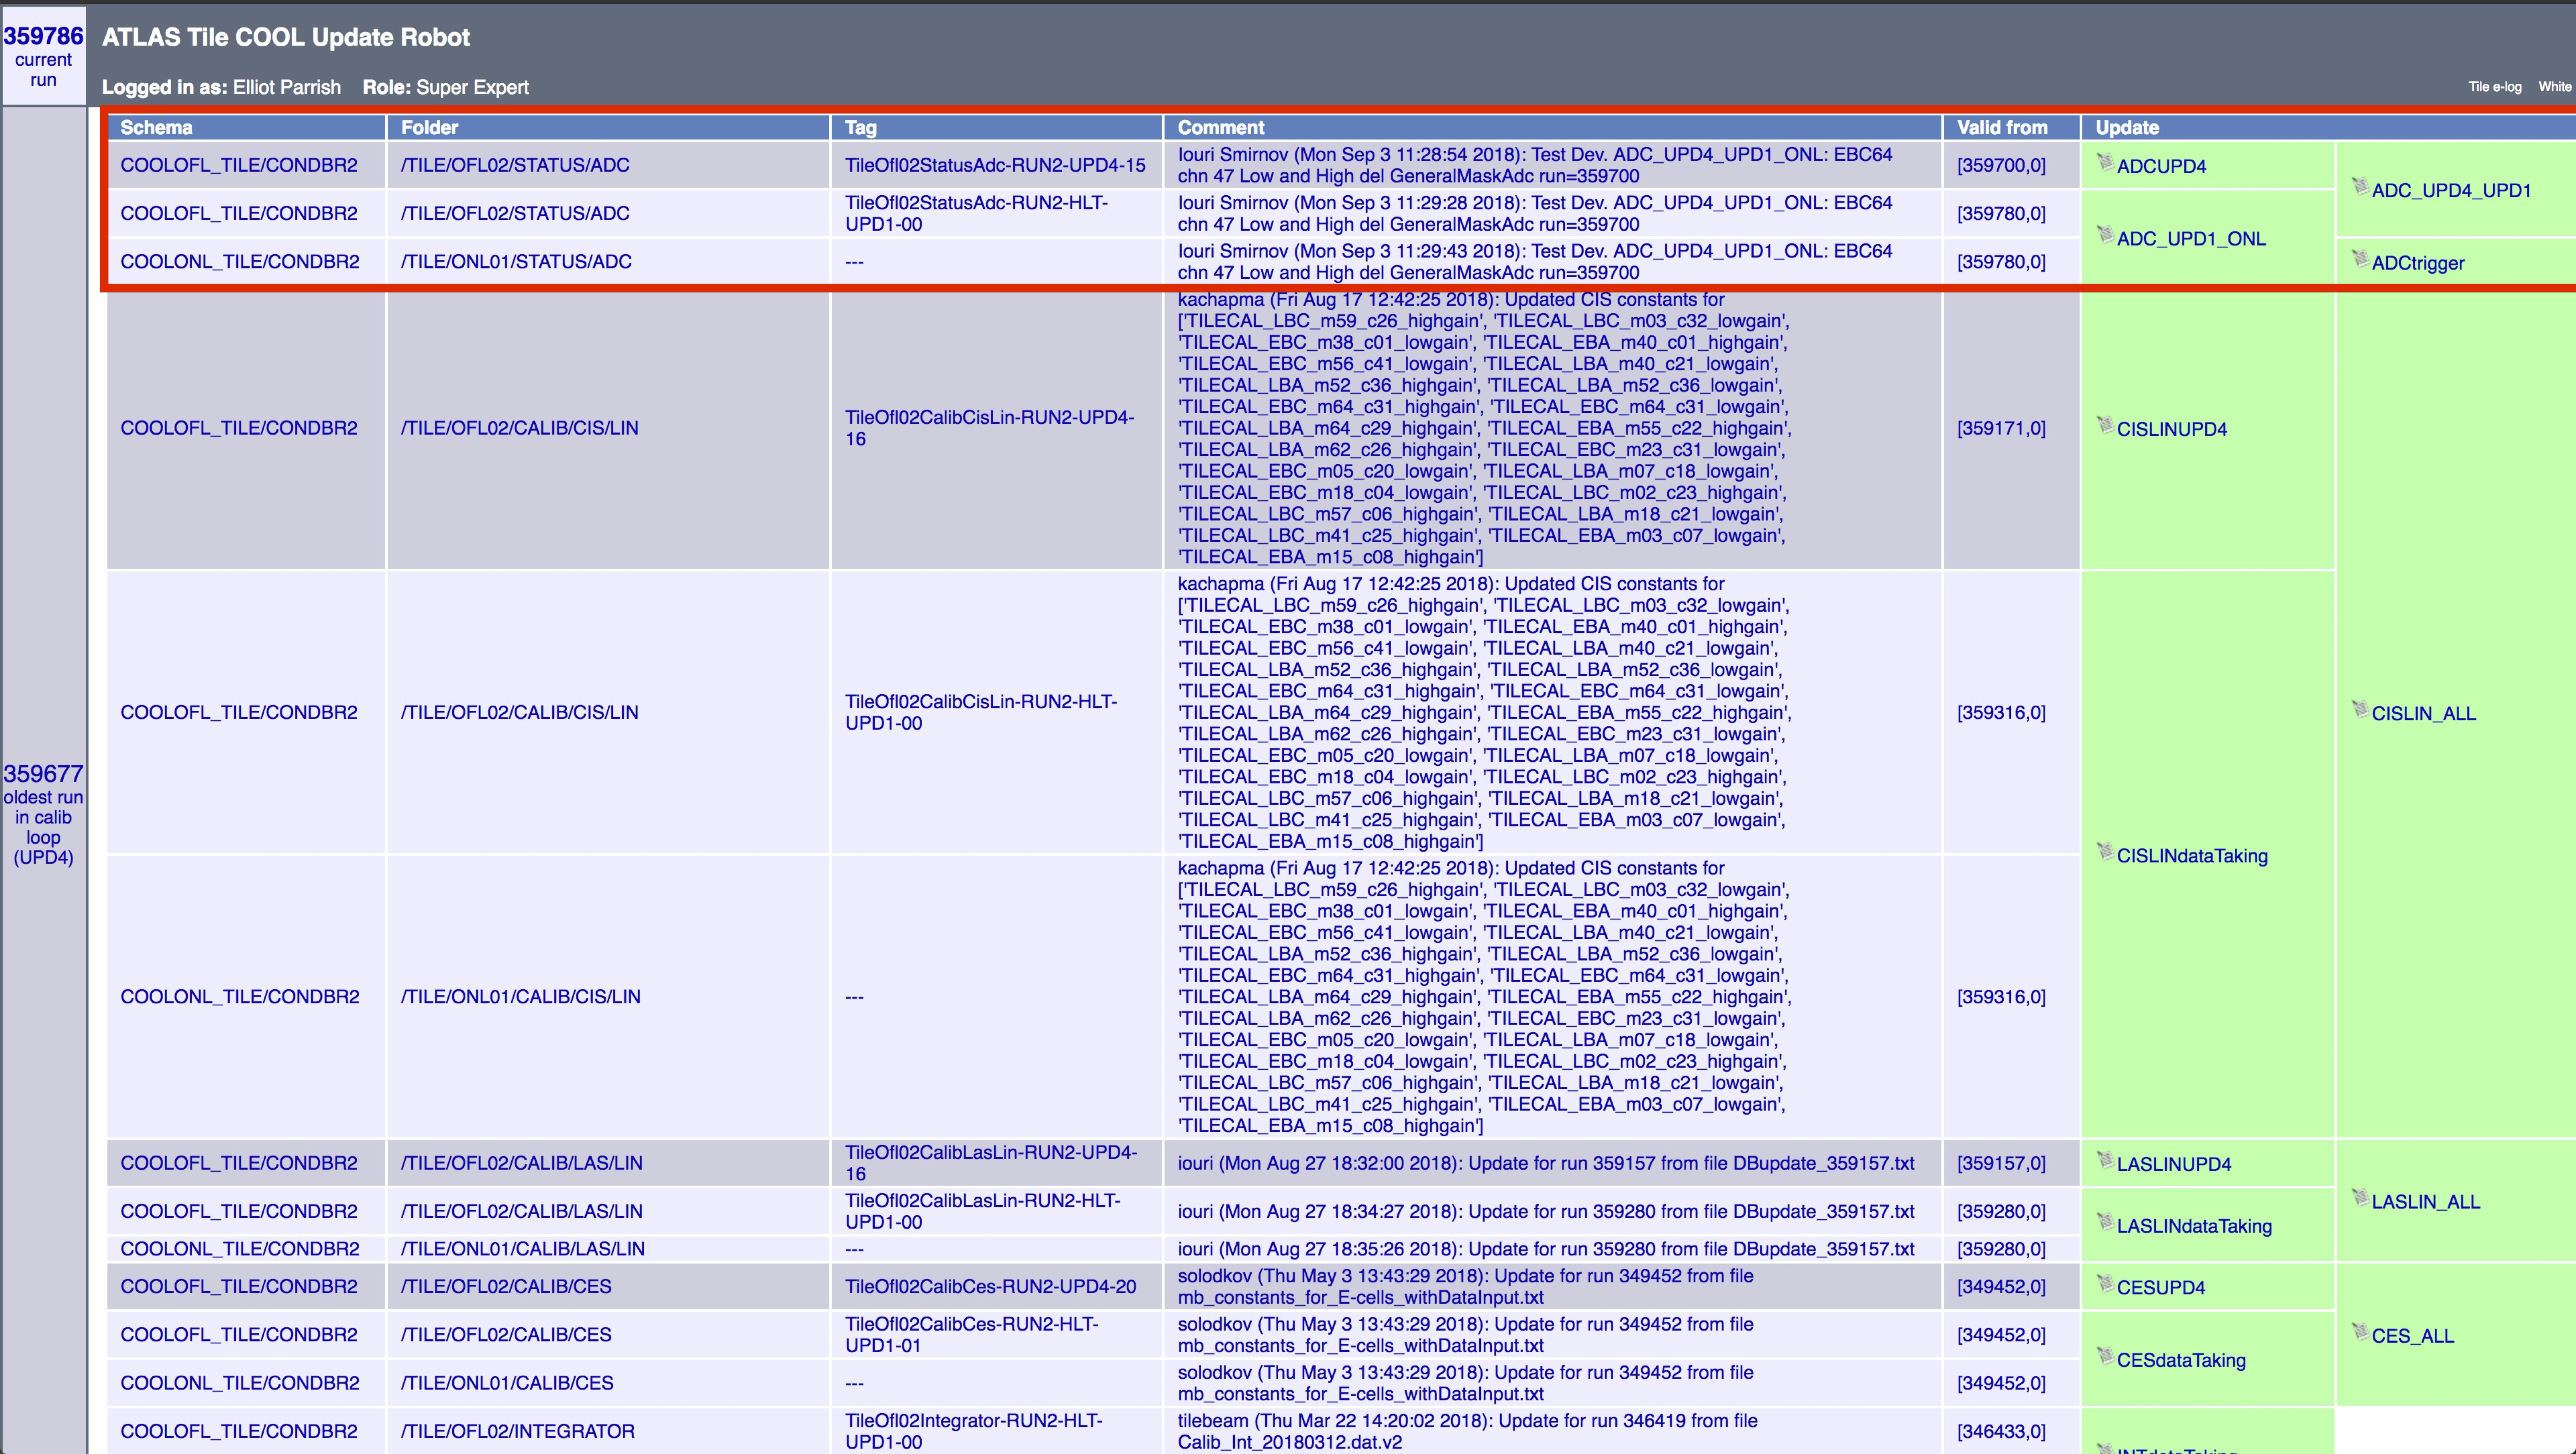
\includegraphics[width=.95\textwidth,keepaspectratio=true]{TileRobotTrippleUpdateScreenShot.png}
      \end{columns}
    \end{frame}

  \subsection{Data Quality}

    \begin{frame}[t]{Tile Data Quality Co-Coordinator}
      \begin{columns}
        \column{.5\textwidth}
        \begin{itemize}
          \item Took over from Puja Saha at the end of Summer 2018 until Fall 2021
          \item Workload was dependent on ATLAS data taking schedule
          % \begin{itemize}
            \item During data taking
            \begin{itemize}
              \item 48 hours to investigate issues and take action before full processing of runs
              \item Coordinate two shifters (Data Quality Validator and Data Quality Leader)
              \item Personally sign off every run and tag with appropriate defects
            \end{itemize}
          % \end{itemize}
        \end{itemize}

        \column{.5\textwidth}
        \begin{itemize}
          \item During Long Shutdown 2
          \begin{itemize}
            \item Coordinate two shifters (Data Quality Validator and Data Quality Leader)
            \begin{itemize}
              \item Fill in when needed
            \end{itemize}
            \item Reconstruction codebase was restructured to support multithreading
            \begin{itemize}
              \item Signed off many tests
              \item Finished Summer 2021
            \end{itemize}
            \item Reprocessing of Run-2 data
            \begin{itemize}
              \item Revised Tile channel statuses for 2018, applied changes from previous DQ Co-Coord
              \item Finalized Fall 2021
            \end{itemize}
          \end{itemize}
        \end{itemize}
      \end{columns}
    \end{frame}

    \begin{frame}[t]{Tile Data Quality Run-2 Performance}
      \begin{columns}
        \column{.5\textwidth}
          \begin{itemize}
            \item As DQ Co-Coordinator I was responsible for channel and cell status
            \begin{itemize}
              \item (Un)Masking based on performance
              \item Various status flags used in reconstruction
            \end{itemize}
          \end{itemize}
          \centering
          \includegraphics[height=.45\textheight,keepaspectratio=true]{masked_cells_timeline_2018.png}
        \column{.5\textwidth}
          \begin{itemize}
              \item Tile boasted 100\% Data Quality Efficiency for 2018
              \begin{itemize}
                \item For all of Run-2, we were 99.65\% efficient
              \end{itemize}
              \item Paper detailing ATLAS Run-2 data quality performance published in Journal of Instrumentation 
              \begin{itemize}
                \item \href{https://iopscience.iop.org/article/10.1088/1748-0221/15/04/P04003}{\textcolor{blue}{{\tiny DOI: 10.1088/1748-0221/15/04/P04003}}}
              \end{itemize}
            \end{itemize}
          \centering
          \includegraphics[height=.3\textheight,keepaspectratio=true]{DataQualityLosesRun2.png}
        \end{columns}
    \end{frame}

  \subsection{Maintenance }

    \begin{frame}[t]{Tile Maintenance}
      \begin{columns}
        \column{.5\textwidth}
        \begin{itemize}
          \item At the start of the pandemic, many experts had to leave the CERN area
          \begin{itemize}
            \item I voluntered to help with transition of new CIS/Maintenance technicians
            \item During Long Shutdown 2, Tile performed maintenance 
            \begin{itemize}
              \item Repaired/replaced electronics, PMTs, added cooling isolation valves, etc.
            \end{itemize} 
            \item I helped install the demonstrator module that is a proof of concept for future Tile upgrades
              \begin{itemize}
                \item Will remain inside of Tile for Run-3 data collection
              \end{itemize}
          \end{itemize}
        \end{itemize}

        \column{.5\textwidth}
        \centering
        \includegraphics[height=.3\textheight,keepaspectratio=true]{OnLBA14.jpg}
        \includegraphics[height=.3\textheight,keepaspectratio=true]{TileElectronicsJalal.jpg}
        \includegraphics[height=.5\textheight,keepaspectratio=true]{TileMaintenanceTeamJune2020.png}
      \end{columns}
    \end{frame}

    \begin{frame}[t]{ACES Database Update}
      \begin{columns}
        \column{.70\textwidth}
          \begin{itemize}
          \item ATLAS Central Equipment System (\href{https://atlas-glance.cern.ch/atlas/aces/}{\textcolor{blue}{ACES}})
            \begin{itemize}
              \item A central database for all racks, cables, detector parts, and general equipment
            \end{itemize}
          \item Needed to update with latest information since Long Shutdown 2 was coming to an end
            \begin{itemize}
              \item Myself and Michaela Mlynáriková were tasked with inputting new information
            \end{itemize}
          \item Finished in Fall 2021
          \end{itemize}
          \centering
          \includegraphics[height=.39\textheight,keepaspectratio=true]{Hard_At_Work.jpg}

        \column{.15\textwidth}
          \begin{itemize}
          \item USA15
          \end{itemize}
          % \centering
          \includegraphics[height=.7\textheight,keepaspectratio=true]{Y.04-16.A1.jpeg}

          \column{.15\textwidth}
          \begin{itemize}
          \item ACES
          \end{itemize}
          % \centering
          \includegraphics[height=.6\textheight,keepaspectratio=true]{Y.04-16.A1_ACES.png}
      \end{columns}
    \end{frame}

  \subsection{Test Beams}
    \begin{frame}[t]{Tile Test Beams}
      \begin{columns}
      \column{.6\textwidth}
      \begin{itemize}
        \item Participated in two test beams for Tile
        \begin{itemize}
          \vspace{-.185cm}
          \item Summer 2018
          \item Fall 2021
        \end{itemize}
        \item In both, collected data for various electronics upgrades
        \begin{itemize}
          \item Set beam energy and beam type from an offshoot of the Super Proton Synchrotron (SPS)
          \item Moved Tile module to collect spatial response
        \end{itemize}
        \item Helped setup test beam site in 2021
        \begin{itemize}
          \item Tracing down cables, connected various calibration detectors
          \item Installed electronics and PMTs to be tested
        \end{itemize}
      \end{itemize}
      \column{.4\textwidth}
        \includegraphics[width=.9\textwidth,keepaspectratio=true]{TileTestBeamSetup_Michaela_Will_Me.jpg}
        \includegraphics[width=.9\textwidth,keepaspectratio=true]{CherenkovDetector_Andrew_Will_Me.jpg}
      \end{columns}
    \end{frame}

\section{\HpLong Analysis }

  \subsection{Theory}

    \begin{frame}[t]{Search for \HpLong using the ATLAS experiment}
      \begin{columns}
      \column{.75\textwidth}
      \begin{itemize}
        \item Many extensions to the Higgs sector imply the existence of charged scalars (2HDM, NMSMM, Triplet, etc.)
        \begin{itemize}
          \item $H^{\pm} \to \tau^{\pm}\nu_{\tau}$ remains significant for high $\mathrm{tan} \beta$
          \begin{itemize}
            \item $\mathrm{tan} \beta$ defined as the ratio of the  vacuum expectation values of the two doublets
          \end{itemize}
        \end{itemize}
        \item At the LHC, theoretical production mode of $H^{\pm}$ is mainly in top-quark decays or in association with a top-quark ($t$)
        \begin{itemize}
          \item $H^{\pm}$ production mode is dependent on $m_{H^{\pm}}$
          \item Analysis is sensitive for low mass $(m_{H^{\pm}} < m_{t})$, intermediate mass $(m_{H^{\pm}} \simeq m_{t})$, and high mass $(m_{H^{\pm}} > m_{t})$
        \end{itemize}
        \item Two sub-channels based on the decay mode of associated $t$ 
        % \begin{itemize}
        %   \item $t \rightarrow jets$ 
        %     \begin{itemize}
        %       \item Sensitive at high mass due to higher $W \rightarrow q\bar{q}$ BR
        %     \end{itemize}
        %     \item $t \rightarrow \ell$
        %     \begin{itemize}
        %       \item Sensitive at low mass due to single lepton triggers
        %     \end{itemize}
        % \end{itemize}
      \end{itemize}
      \vspace{-.3cm}
      \centering
      \begin{table}
          % \small
          \resizebox{.9\textwidth}{!}{
          \rowcolors{1}{}{NIUgray}
          \begin{tabular}{c | c}
          \textbf{$t \rightarrow jets$ } & $t \rightarrow \ell$ \\
          \hline \hline
          Sensitive at high mass due to higher $W \rightarrow q\bar{q}$ BR & Sensitive at low mass due to single lepton triggers \\
          \end{tabular}}
        \end{table}

      \column{.25\textwidth}
      \centering
      % \includegraphics[width=.74\textwidth,keepaspectratio=true]{double_resonant_production_low_mass.png}
      % \includegraphics[width=.74\textwidth,keepaspectratio=true]{SingleResonant.pdf}
      % \includegraphics[width=.74\textwidth,keepaspectratio=true]{non_resonant_production_intermediate_mass.png}
      % \includegraphics[width=.74\textwidth,keepaspectratio=true]{NonResonant.pdf}
      % \includegraphics[width=.74\textwidth,keepaspectratio=true]{single_resonant_production_large_mass.png}
      % \includegraphics[width=.74\textwidth,keepaspectratio=true]{DoubleResonant.pdf}
      \includegraphics[width=1.15\linewidth,keepaspectratio=true]{Charged_Higgs_BR.png}
      \includegraphics[width=1.15\linewidth,keepaspectratio=true]{HPlus_taunu_tanB.png}
      \end{columns}
    \end{frame} 

    \begin{frame}[t]{Analysis Overview}
      \begin{columns}[t]

        \column{.75\textwidth}
            \vspace{-20mm}
            \begin{itemize}
              \item Search for singly charged $H^{\pm}$ decaying to $\tau_{had} + \nu$ over a wide mass range
                \begin{itemize}
                  \item Low mass $ (m_{H^{\pm}} < m_{t})$:
                  % \begin{itemize}
                  %   \item $90 \leq m_{H^{\pm}} \leq 130$ GeV
                  % \end{itemize}
                  \item Intermediate mass*  $(m_{H^{\pm}} \simeq m_{t})$
                  % \begin{itemize}
                  %   \item $140 \leq m_{H^{\pm}} \leq 190$ GeV
                  % \end{itemize}
                  \item High mass $(m_{H^{\pm}} > m_{t})$
                  % \begin{itemize}
                  %   \item $200 \leq m_{H^{\pm}} \leq 2000$ GeV
                  % \end{itemize}
                \end{itemize}
              % \item Associated $\tau$ is required to decay hadronically
              \item Dominant backgrounds
              \vspace{-3mm}
            \begin{table}
              \tiny
              \resizebox{\linewidth}{!}{
              \rowcolors{1}{}{NIUgray}
              \begin{tabular}{l | l}
              \textbf{Backgrounds w/ prompt hadronic $\tau$} & \textbf{Backgrounds w/ fake $\tau$} \\
              \hline \hline
              $t\bar{t}$ estimated with MC       & Fake $j \rightarrow \tau$ estimated with data driven fake factor method \\
              $V+jets$ estimated with MC         & Fake $\ell \rightarrow \tau$ estimated with MC, validated on $Z \rightarrow ee$\\
              VV estimated with MC & \\
              \end{tabular}}
            \end{table}
            \item MVA score is used as the final discriminant 
            % \item This talk will cover $36.1 \mathrm{fb}^{-1}$ and the current edition of this analysis
            \end{itemize}

            \vspace{-.45cm}
            \begin{table}
              \footnotesize
              \resizebox{\linewidth}{!}{
              \rowcolors{1}{}{NIUgray}
              \begin{tabular}{l | l | l | l | l | l | l | l | l | l | l | l} 
                \textbf{Sub-Channel} \\ \hline \hline
                \textbf{$\tau + jets$ SR } & $E^{miss}_{T}$ Trigger & \specialcell{1 hadronic $\tau$ \\ $p_{T}^{\tau} > 40$ GeV} & \specialcell{0 $\ell$ (e or $\mu$) \\ $p_{T}^{\ell} > 20$ GeV} & \specialcell{$\geq$ 3 jets \\ $p_{T}^{j} > 25$ GeV} & \specialcell{$\geq$ 1 b-jets \\ $p_{T}^{b-jet} > 25$ GeV}  & \Etm$ > 150$ GeV & $m_{T}(\tau,E^{miss}_{T}) > 50$ GeV \\ \hline
                \textbf{$\tau + \ell$ SR} & Single Lepton Trigger &   \specialcell{1 hadronic $\tau$ \\ $p_{T}^{\tau} > 30$ GeV} & \specialcell{1 $\ell$ (e or $\mu$) \\ $p_{T}^{\ell} > 30$ GeV} & \specialcell{$\geq$ 1 jet  \\ $p_{T}^{j} > 25$ GeV} & \specialcell{$\geq$ 1 b-jets \\  $p_{T}^{b-jet} > 25$ GeV} & \Etm$ > 50$ GeV & Opposite sign $\tau$ and $\ell$ \\ \hline
              \end{tabular}}
            \end{table}

            % \vspace{.3cm}
            \tiny *: First time probed experimentally \textcolor{blue}{\href{https://link.springer.com/article/10.1007/JHEP09(2018)139}{JHEP 09(2018)139}}

          \column{.25\textwidth}
          \centering
          \tiny
          \fcolorbox{black}{white}{\includegraphics[width=.72\textwidth,keepaspectratio=true]{double_resonant_production_low_mass.png}}
          $m_{H^{\pm}} < m_{t}$
          \fcolorbox{black}{white}{\includegraphics[width=.72\textwidth,keepaspectratio=true]{non_resonant_production_intermediate_mass.png}}
          $m_{H^{\pm}} \simeq m_{t}$
          \fcolorbox{black}{white}{\includegraphics[width=.72\textwidth,keepaspectratio=true]{SingleResonant.pdf}}
          $m_{H^{\pm}} > m_{t}$
        \end{columns}
      \end{frame}

  \subsection{Previous Result}

    \begin{frame}[t]{\href{https://link.springer.com/article/10.1007/JHEP09(2018)139}{JHEP 09(2018)139} BDT Scores in Signal Regions}
        \begin{columns}[t]
          \column{.33\textwidth}
          \includegraphics[height=.4\textheight,keepaspectratio=true]{taujet_SR_2018/taujet_SR_90to120_2018.png}
          \includegraphics[height=.4\textheight,keepaspectratio=true]{tauel_SR_2018/tauel_SR_90to120_2018.png}
          % \includegraphics[height=.33\textheight,keepaspectratio=true]{taumu_SR_2018/taumu_SR_90to120_2018.png}

          % \column{.2\textwidth}
          % \includegraphics[height=.26\textheight,keepaspectratio=true]{taujet_SR_2018/taujet_SR_130to160_2018.png}
          % \includegraphics[height=.26\textheight,keepaspectratio=true]{tauel_SR_2018/tauel_SR_130to160_2018.png}
          % \includegraphics[height=.26\textheight,keepaspectratio=true]{taumu_SR_2018/taumu_SR_130to160_2018.png}

          \column{.33\textwidth}
          \includegraphics[height=.4\textheight,keepaspectratio=true]{taujet_SR_2018/taujet_SR_160to180_2018.png}
          \includegraphics[height=.4\textheight,keepaspectratio=true]{tauel_SR_2018/tauel_SR_160to180_2018.png}
          % \includegraphics[height=.33\textheight,keepaspectratio=true]{taumu_SR_2018/taumu_SR_160to180_2018.png}


          \column{.33\textwidth}
          \includegraphics[height=.4\textheight,keepaspectratio=true]{taujet_SR_2018/taujet_SR_200to400_2018.png}
          \includegraphics[height=.4\textheight,keepaspectratio=true]{tauel_SR_2018/tauel_SR_200to400_2018.png}
          % \includegraphics[height=.33\textheight,keepaspectratio=true]{taumu_SR_2018/taumu_SR_200to400_2018.png}


          % \column{.2\textwidth}
          % \includegraphics[height=.26\textheight,keepaspectratio=true]{taujet_SR_2018/taujet_SR_500to2000_2018.png}
          % \includegraphics[height=.26\textheight,keepaspectratio=true]{tauel_SR_2018/tauel_SR_500to2000_2018.png}
          % \includegraphics[height=.26\textheight,keepaspectratio=true]{taumu_SR_2018/taumu_SR_500to2000_2018.png}
        \end{columns}
      \end{frame}

    \begin{frame}{\href{https://link.springer.com/article/10.1007/JHEP09(2018)139}{\textcolor{blue}{JHEP 09(2018)139}} Limits}
      \begin{columns}
        \column{.5\textwidth}
        \centering
        \includegraphics[width=.65\textwidth,keepaspectratio=true]{Limits/Combined_low_NoLabel_2018.png}
        % \column{.25\textwidth}
        \includegraphics[width=.65\textwidth,keepaspectratio=true]{Limits/Combined_CrossSection_2018.png}
        \column{.5\textwidth}
        \centering
        \includegraphics[width=\textwidth,keepaspectratio=true]{Limits/tanB_Limit_2018.png}
      \end{columns}
    \end{frame}

  \subsection{Current Analysis}

    \begin{frame}[t]{Updates to analysis since last publication}
      \begin{columns}
      \column{.6\linewidth}
        \begin{itemize}
          % \item Last publication using 2015+2016 data: \href{https://link.springer.com/article/10.1007/JHEP09(2018)139}{\textcolor{blue}{JHEP 09(2018)139}}
          % \item Using full Run-2 dataset
          \item Signal mass range extended 
          \begin{itemize}
            \item Previous: $90 \leq m_{H^{\pm}} \leq 2000$ GeV
            \item Current:  $80 \leq m_{H^{\pm}} \leq 3000$ GeV
          \end{itemize}
          \item Signal filtering applied in order to effectively increase the statistics in the signal regions
          \item New analysis framework centered around using modern Machine Learning tools
          \item Investigating new multivariate analysis techniques
          \item Updated derivations
          \vspace{-3.5mm}
          \begin{multicols}{2}
            \begin{itemize}
              \tiny
              \item RNN $\tau$ ID recommendations
              \item Updated b-tagging recommendations
              \item PFlow jets
              \item Latest Combined Performance recommendations
            \end{itemize}
          \end{multicols}
        \end{itemize}

      \column{.4\linewidth}
      \includegraphics[width=1.1\textwidth,keepaspectratio=true]{intlumivstimeRun2.png}
      \end{columns}
    \end{frame}

      \begin{frame}[t]{$\tau+jets$ Background Modeling}
        % PLOTS FROM TAUJET
          \begin{columns}[t]

          \column{.25\textwidth}
          \includegraphics[height=.45\textheight,keepaspectratio=true]{taujet_1p_3p/v09/tau_0_pt_TTBAR.png}
          \includegraphics[height=.45\textheight,keepaspectratio=true]{taujet_1p_3p/v09/tau_0_pt_WJETS.png}

          \column{.25\textwidth}
          \includegraphics[height=.45\textheight,keepaspectratio=true]{taujet_1p_3p/v09/met_et_TTBAR.png}
          \includegraphics[height=.45\textheight,keepaspectratio=true]{taujet_1p_3p/v09/met_et_WJETS.png}

          \column{.25\textwidth}
          \includegraphics[height=.45\textheight,keepaspectratio=true]{taujet_1p_3p/v09/tau_0_pt_BVETO.png}
          \includegraphics[height=.45\textheight,keepaspectratio=true]{taujet_1p_3p/v09/tau_0_pt_bveto100.png}


          \column{.25\textwidth}
          \includegraphics[height=.45\textheight,keepaspectratio=true]{taujet_1p_3p/v09/met_et_BVETO.png}
          \includegraphics[height=.45\textheight,keepaspectratio=true]{taujet_1p_3p/v09/tau_0_met_mt_bveto100.png}
          % \includegraphics[height=.45\textheight,keepaspectratio=true]{taujet_1p_3p/v09/met_et_bveto100.png}

        \end{columns}
      \end{frame}

      \begin{frame}[t]{$\tau+\ell$ Background Modeling}
        % PLOTS FROM TAULEP
        \begin{columns}[t]

          \column{.25\textwidth}
          \includegraphics[height=.45\textheight,keepaspectratio=true]{taulep_1p_3p/v09/met_et_DILEP_BTAG.png}
          \includegraphics[height=.45\textheight,keepaspectratio=true]{taulep_1p_3p/v09/tau_0_pt_TAUEL_BVETO.png}

          \column{.25\textwidth}
          \includegraphics[height=.45\textheight,keepaspectratio=true]{taulep_1p_3p/v09/lep_0_pt_DILEP_BTAG.png}
          \includegraphics[height=.45\textheight,keepaspectratio=true]{taulep_1p_3p/v09/lep_0_pt_TAUEL_BVETO.png}

          \column{.25\textwidth}
          \includegraphics[height=.45\textheight,keepaspectratio=true]{taulep_1p_3p/v09/tau_0_pt_SS_TAUEL.png}
          \includegraphics[height=.45\textheight,keepaspectratio=true]{taulep_1p_3p/v09/tau_0_pt_SS_TAUMU.png}


          \column{.25\textwidth}
          \includegraphics[height=.45\textheight,keepaspectratio=true]{taulep_1p_3p/v09/lep_0_pt_SS_TAUEL.png}
          \includegraphics[height=.45\textheight,keepaspectratio=true]{taulep_1p_3p/v09/lep_0_pt_SS_TAUMU.png}

        \end{columns}
      \end{frame}

  \subsection{PNN vs BDT}

    \begin{frame}[t]{Parameterized Neural Networks}
      \begin{columns}
      \column{.7\textwidth}
      \begin{itemize}
        \small
        \item Parameterized Neural Networks (PNNs) can be trained and evaluated on an entire mass range
        \begin{itemize}
          \item Detailed information here: \href{https://arxiv.org/abs/1601.07913}{\textcolor{blue}{arXiv:1601.07913}}
        \end{itemize}
        \item Trained using Tensorflow backend for Keras
        \item $m_{H^{\pm}}$ is used as an input feature of the model
        \item Allows one model to be used across entire $m_{H^{\pm}}$ mass range
        \item Separate models trained on 1 prong and 3 prong $\tau$
        \item $\tau+\ell$ channel is trained inclusive for $\tau+e$ and $\tau+\mu$
        \item Evaluated on single mass points
        % \item Many ongoing studies
        %   \begin{itemize}
        %     \item High level vs low level input features
        %     \item Cartesian vs $(\eta,\phi)$ coordinates
        %     \item Hyperparameter optimization
        %   \end{itemize}
      \end{itemize}
      \column{.3\textwidth}
      % \small
      % \includegraphics[width=\textwidth,keepaspectratio=true]{taulep_fullmass.pdf}
      \footnotesize
      % NETWORK IMAGE
      \centering
      \includegraphics[width=\textwidth,keepaspectratio=true]{NN_Diagram.png}  
      % Limits in $\tau+lep$ comparing BDT, NN, and PNN
      % PNN contains Upsilon variable
      % NNs in this plot are non parameterized, using 5 mass bins
      % \includegraphics[width=\textwidth,keepaspectratio=true]{PNN_Preliminary_Pawel_Feb_20_2020.png}
      \end{columns}
    \end{frame}

    \begin{frame}[t]{Parameterized Neural Network vs Boosted Decision Tree}
      \begin{itemize}
        \item One model for entire mass range makes analysis less computationally expensive
        \item PNN can be evaluated on mass points that are not simulated
        \item Limits are preliminary, many fixes and changes have been implemented since
      \end{itemize}
      \begin{columns}
      \column{.5\textwidth}
      \centering
      \includegraphics[width=\textwidth,keepaspectratio=true]{Limits/exp_limit_log_taujet.pdf}
      \column{.5\textwidth}
      \centering
      \includegraphics[width=\textwidth,keepaspectratio=true]{Limits/Exp_Limit_log_taulep.eps}
      \end{columns}
    \end{frame}

  \subsection{Input Feature Ranking}

    \begin{frame}[t]{Feature Ranking}%{Local Interpretable Model-agnostic Explanations}
      \begin{itemize}
        \item Linear correlations between input features
          \begin{itemize}
            \item Neural Networks often do not work very well with linearly correlated variables
          \end{itemize}
        \item Produced features rankings via \href{https://github.com/marcotcr/lime}{\textcolor{blue}{Local Interpretable Model-agnostic Explanations (LIME)}}
        \begin{itemize}
          \item LIME explains an instance (\Cross) by sampling nearby points with classifier, weighting by distance from \Cross
          \item LIME then learns a linear model which explains the decision locally (dashed line)
        \end{itemize}
      \end{itemize}
          \centering
          \includegraphics[width=.35\textwidth,keepaspectratio=true]{limeToyExplanation.png}
    \end{frame}

    \begin{frame}{Input Feature Linear Correlations}[t]
      \centering
      \includegraphics[height=.95\textheight,keepaspectratio=true]{features_correlation_model_GB100_channel_taulep_mass_80to3000_ntracks_1_nfolds_5_fold_0_nvars_19.eps}
    \end{frame}

    \begin{frame}{Comparing to Previous Analysis}
      \begin{columns}[t]
      \column{.3\textwidth}
        \begin{itemize}
          \item Given bkg event
        \end{itemize}
        \includegraphics[width=.9\linewidth,keepaspectratio=true]{PawelModel_HPlus80_BKG.png}
      \column{.3\textwidth}
        \begin{itemize}
          \item Given signal event
        \end{itemize}
        \includegraphics[width=.9\linewidth,keepaspectratio=true]{PawelModel_HPlus80_SIG.png}
      \column{.3\textwidth}
        \begin{itemize}
          \item Last analysis BDT (low mass)
        \end{itemize}
        \includegraphics[width=.9\linewidth,keepaspectratio=true]{IntNotefeatureRanking.png}

      \end{columns}
    \end{frame}

    \begin{frame}{$H^{\pm} \rightarrow \tau\nu$ Expected Limits PNN Studies}
      \centering
      % \includegraphics[height=.9\textheight,keepaspectratio=true]{taulep_fullmass.pdf}
      \small
      % \begin{itemize}
      %   \item Limits with previous ntuples shown
      % \end{itemize}
      \begin{columns}
          \column{.4\textwidth}
          \includegraphics[width=\textwidth,keepaspectratio=true]{Limits/exp_limit_log_1Pvs3P_taujet.pdf} \\
          \centering
          $\tau+jets$
          \column{.6\textwidth} 
          \centering
          \includegraphics[width=.55\textwidth,keepaspectratio=true]{Limits/taulep_fullmass_noCRTop_13p_lowLVL.eps} \\
          \includegraphics[width=.55\textwidth,keepaspectratio=true]{Limits/exp_limit_log_taulep_Coordinates.eps} \\
          \centering
          $\tau+\ell$
      \end{columns}
    \end{frame}

  \subsection{PNN HPO}

    \begin{frame}[t]{PNN Hyperparameter Optimization}
      \begin{itemize}
        \item Performed in the $\tau+\ell$ sub-channel
        \item Used area under curve (AUC) of scores as figure of merit
        \begin{itemize}
          \item Averaged over 5 kfolds, standard deviation is taken from kfolds
          % \item AUC from 80 GeV to 500 GeV to optimize for low mass
        \end{itemize}
          \item Used early stopping for training
          \begin{itemize}
            \item $\Delta_{min}=0.00001$ and a patience of 10
            \item Best weights were kept
          \end{itemize}
        \item To make hyperparameter optimization (HPO) go quicker, ran multiple small grids of hparams
        \begin{itemize}
          \item Scan over activation functions and loss functions
          % \begin{itemize}
          %   \item Binary crossentropy gave best result
          % \end{itemize}
          \item Scan over dropout value
          % \begin{itemize}
          %   \item 0.1 gave best result
          % \end{itemize}
          \item Scan over activation function
          % \begin{itemize}
          %   \item LeakyReLU was best
          % \end{itemize}
          \item Scan over LeakyReLU $\alpha$
          % \begin{itemize}
          %   \item $\alpha=0.05$ gave best results
          % \end{itemize}
          \item Fixed alpha over more widths and depths
          \begin{itemize}
            \item AUC from 80 GeV to 500 GeV to optimize for low mass
          \end{itemize}
        \end{itemize}
      \end{itemize}
    \end{frame}

    \begin{frame}[t]{PNN Hyperparameter Optimization}
    \begin{columns}
        \column{.4\textwidth}

        \begin{table}
          \resizebox{\linewidth}{!}{
          \rowcolors{1}{}{NIUgray}
            \begin{tabular}{c | c | c | c}
            Parameter  \\
            \hline
            activation function & softsign & relu & LeakyReLU \\ \hline
            loss function & \fcolorbox{red}{white}{binary crossentropy} & mean squared error & mean absolute error \\ \hline
            width & 32 & & \\ \hline
            depth & 10 & & \\ \hline
            \end{tabular}}
        \end{table}


        \begin{table}
          \resizebox{.75\linewidth}{!}{
          \rowcolors{1}{}{NIUgray}
            \begin{tabular}{c | c | c | c}
            Parameter  \\
            \hline
            width & 8 & 16 & 32 \\ \hline
            depth & 3 & 5 & 10 \\ \hline
            dropout & \fcolorbox{red}{white}{0.1} & 0.3 & \\ \hline
            activation function & softsign & & \\ \hline
            loss function & binary crossentropy & & \\ \hline 
            \end{tabular}}
        \end{table}

        \begin{table}
          \resizebox{.75\linewidth}{!}{
          \rowcolors{1}{}{NIUgray}
            \begin{tabular}{c | c | c | c}
            Parameter  \\
            \hline
            width & 32 & 64 & 128 \\ \hline
            depth & 2 & 3 & 4 \\ \hline
            dropout & 0.1 & & \\ \hline
            activation function & softsign & relu & \fcolorbox{red}{white}{LeakyReLU} \\ \hline
            batch size & 1025 &  & \\ \hline
            loss function & binary crossentropy  & & \\
            \end{tabular}}
        \end{table}


        \column{.6\textwidth}

        \begin{table}
          \resizebox{.75\linewidth}{!}{
          \rowcolors{1}{}{NIUgray}
          \begin{tabular}{c | c | c | c | c}
          Parameter  \\ 
          \hline
          width & 32 & 64 & 128 & \\ \hline
          depth & 2 & 3 & 4 &  \\ \hline
          $\alpha$ & 0.01 & \fcolorbox{red}{white}{0.05} & 0.001 & 0.005 \\ \hline
          batch size & 1024 & & & \\ \hline
          dropout & 0.1 & & & \\ \hline
          activation function & LeakyReLU &  &  &  \\ \hline
          loss function & binary crossentropy & & &  \\ \hline
          \end{tabular}}
        \end{table}

        \begin{table}
          \resizebox{.75\linewidth}{!}{
          \rowcolors{1}{}{NIUgray}
          \begin{tabular}{c | c | c | c | c}
          Parameter  \\ 
          \hline
          width & 32 & 64 & \fcolorbox{red}{white}{128} & 256 \\
          depth & 2 & \fcolorbox{red}{white}{3} & 4 & 5 \\
          batch size & 1024 &  & & \\ \hline
          dropout & 0.1 &  &  &  \\ \hline
          activation function & LeakyReLU &  &  &  \\ \hline
          $\alpha$ & 0.05 &  &  &  \\ \hline
          loss function & binary crossentropy & & &  \\ \hline
          \end{tabular}}
        \end{table}
      \end{columns}
    \end{frame}

    \begin{frame}[t]{PNN Hyperparameter Optimization Search}
      \begin{itemize}
        \item LeakyReLU activation function has an $\alpha$ parameter
        \item Slope of negative portion
        \begin{itemize}
          \item Prevents neurons from "dying" by allowing negative weight values
        \end{itemize}
        \item Standard relu is where $\alpha=0$
      \end{itemize}
      \centering
      \includegraphics[height=.4\textheight,keepaspectratio=true]{Activation_prelu.svg.png}
    \end{frame}

    \begin{frame}
      \begin{columns}
      \column{.25\textwidth}
      \includegraphics[height=.25\textheight,keepaspectratio=true]{AUC_Plots/model_GB_1024_channel_taulep_mass_80to3000_ntracks_1_nfolds_5_fold_4_nvars_19_batch_size_1024_epochs_1000_dense_layer_size_32_activation_function_LeakyRelu_depth_2_loss_binary_crossentropy_dropout_0.1_alpha_0.05.eps}
      \includegraphics[height=.25\textheight,keepaspectratio=true]{AUC_Plots/model_GB_1024_channel_taulep_mass_80to3000_ntracks_1_nfolds_5_fold_4_nvars_19_batch_size_1024_epochs_1000_dense_layer_size_32_activation_function_LeakyRelu_depth_3_loss_binary_crossentropy_dropout_0.1_alpha_0.05.eps}
      \includegraphics[height=.25\textheight,keepaspectratio=true]{AUC_Plots/model_GB_1024_channel_taulep_mass_80to3000_ntracks_1_nfolds_5_fold_4_nvars_19_batch_size_1024_epochs_1000_dense_layer_size_32_activation_function_LeakyRelu_depth_4_loss_binary_crossentropy_dropout_0.1_alpha_0.05.eps}
      \includegraphics[height=.25\textheight,keepaspectratio=true]{AUC_Plots/model_GB_1024_channel_taulep_mass_80to3000_ntracks_1_nfolds_5_fold_4_nvars_19_batch_size_1024_epochs_1000_dense_layer_size_32_activation_function_LeakyRelu_depth_5_loss_binary_crossentropy_dropout_0.1_alpha_0.05.eps}

      \column{.25\textwidth}
      \includegraphics[height=.25\textheight,keepaspectratio=true]{AUC_Plots/model_GB_1024_channel_taulep_mass_80to3000_ntracks_1_nfolds_5_fold_4_nvars_19_batch_size_1024_epochs_1000_dense_layer_size_64_activation_function_LeakyRelu_depth_2_loss_binary_crossentropy_dropout_0.1_alpha_0.05.eps}
      \includegraphics[height=.25\textheight,keepaspectratio=true]{AUC_Plots/model_GB_1024_channel_taulep_mass_80to3000_ntracks_1_nfolds_5_fold_4_nvars_19_batch_size_1024_epochs_1000_dense_layer_size_64_activation_function_LeakyRelu_depth_3_loss_binary_crossentropy_dropout_0.1_alpha_0.05.eps}
      \includegraphics[height=.25\textheight,keepaspectratio=true]{AUC_Plots/model_GB_1024_channel_taulep_mass_80to3000_ntracks_1_nfolds_5_fold_4_nvars_19_batch_size_1024_epochs_1000_dense_layer_size_64_activation_function_LeakyRelu_depth_4_loss_binary_crossentropy_dropout_0.1_alpha_0.05.eps}
      \includegraphics[height=.25\textheight,keepaspectratio=true]{AUC_Plots/model_GB_1024_channel_taulep_mass_80to3000_ntracks_1_nfolds_5_fold_4_nvars_19_batch_size_1024_epochs_1000_dense_layer_size_64_activation_function_LeakyRelu_depth_5_loss_binary_crossentropy_dropout_0.1_alpha_0.05.eps}

      \column{.25\textwidth}
      \includegraphics[height=.25\textheight,keepaspectratio=true]{AUC_Plots/model_GB_1024_channel_taulep_mass_80to3000_ntracks_1_nfolds_5_fold_4_nvars_19_batch_size_1024_epochs_1000_dense_layer_size_128_activation_function_LeakyRelu_depth_2_loss_binary_crossentropy_dropout_0.1_alpha_0.05.eps}
      \fcolorbox{red}{white}{\includegraphics[height=.25\textheight,keepaspectratio=true]{AUC_Plots/model_GB_1024_channel_taulep_mass_80to3000_ntracks_1_nfolds_5_fold_4_nvars_19_batch_size_1024_epochs_1000_dense_layer_size_128_activation_function_LeakyRelu_depth_3_loss_binary_crossentropy_dropout_0.1_alpha_0.05.eps}}
      \includegraphics[height=.25\textheight,keepaspectratio=true]{AUC_Plots/model_GB_1024_channel_taulep_mass_80to3000_ntracks_1_nfolds_5_fold_4_nvars_19_batch_size_1024_epochs_1000_dense_layer_size_128_activation_function_LeakyRelu_depth_4_loss_binary_crossentropy_dropout_0.1_alpha_0.05.eps}
      \includegraphics[height=.25\textheight,keepaspectratio=true]{AUC_Plots/model_GB_1024_channel_taulep_mass_80to3000_ntracks_1_nfolds_5_fold_4_nvars_19_batch_size_1024_epochs_1000_dense_layer_size_128_activation_function_LeakyRelu_depth_5_loss_binary_crossentropy_dropout_0.1_alpha_0.05.eps}

      \column{.25\textwidth}
      \includegraphics[height=.25\textheight,keepaspectratio=true]{AUC_Plots/model_GB_1024_channel_taulep_mass_80to3000_ntracks_1_nfolds_5_fold_4_nvars_19_batch_size_1024_epochs_1000_dense_layer_size_256_activation_function_LeakyRelu_depth_2_loss_binary_crossentropy_dropout_0.1_alpha_0.05.eps}
      \includegraphics[height=.25\textheight,keepaspectratio=true]{AUC_Plots/model_GB_1024_channel_taulep_mass_80to3000_ntracks_1_nfolds_5_fold_4_nvars_19_batch_size_1024_epochs_1000_dense_layer_size_256_activation_function_LeakyRelu_depth_3_loss_binary_crossentropy_dropout_0.1_alpha_0.05.eps}
      \includegraphics[height=.25\textheight,keepaspectratio=true]{AUC_Plots/model_GB_1024_channel_taulep_mass_80to3000_ntracks_1_nfolds_5_fold_4_nvars_19_batch_size_1024_epochs_1000_dense_layer_size_256_activation_function_LeakyRelu_depth_4_loss_binary_crossentropy_dropout_0.1_alpha_0.05.eps}
      \includegraphics[height=.25\textheight,keepaspectratio=true]{AUC_Plots/model_GB_1024_channel_taulep_mass_80to3000_ntracks_1_nfolds_5_fold_4_nvars_19_batch_size_1024_epochs_1000_dense_layer_size_256_activation_function_LeakyRelu_depth_5_loss_binary_crossentropy_dropout_0.1_alpha_0.05.eps}

      \end{columns}
    \end{frame}

    \begin{frame}{PNN Hyperparameter Optimization Results}
      \begin{table}
      \resizebox{\linewidth}{!}{
      \rowcolors{1}{}{NIUgray}
      \begin{tabular}{llrrrrrrrrrrrr}
      \toprule
      width & depth &         80 &     80Std &       150 &    150Std &       250 &    250Std &       500 &    500Std &       Avg &    AvgStd &   LowMassAvg &  LowMassAvgStd \\
      \midrule
      128 &     3 &  0.666137 &  0.000000 &  0.814508 &  0.000000 &  0.903123 &  0.000000 &  0.963256 &  0.000000 &  0.887638 &  0.000000 &  0.826145 &    0.096754 \\
       128 &     5 &  0.649154 &  0.000000 &  0.804344 &  0.000000 &  0.907763 &  0.000000 &  0.962846 &  0.000000 &  0.886060 &  0.000000 &  0.823542 &    0.100037 \\
       128 &     4 &  0.659330 &  0.000000 &  0.811707 &  0.000000 &  0.901186 &  0.000000 &  0.963811 &  0.000000 &  0.885833 &  0.000000 &  0.823208 &    0.099379 \\
       128 &     2 &  0.644392 &  0.000000 &  0.807016 &  0.000000 &  0.907517 &  0.000000 &  0.963076 &  0.000000 &  0.885685 &  0.000000 &  0.823139 &    0.100649 \\
        64 &     4 &  0.657593 &  0.005023 &  0.807977 &  0.001327 &  0.905193 &  0.004490 &  0.965553 &  0.001622 &  0.885708 &  0.000177 &  0.823001 &    0.099420 \\
        64 &     2 &  0.652767 &  0.006639 &  0.805184 &  0.002345 &  0.905695 &  0.003172 &  0.965077 &  0.000726 &  0.885537 &  0.000443 &  0.822775 &    0.099628 \\
        64 &     5 &  0.653787 &  0.005006 &  0.804417 &  0.001933 &  0.905833 &  0.003671 &  0.965293 &  0.001398 &  0.885338 &  0.000545 &  0.822360 &    0.099660 \\
        64 &     3 &  0.652007 &  0.006721 &  0.805076 &  0.001760 &  0.904237 &  0.004398 &  0.964922 &  0.001898 &  0.885317 &  0.001074 &  0.822335 &    0.099360 \\
       256 &     5 &  0.653576 &  0.000963 &  0.804396 &  0.003342 &  0.903638 &  0.004193 &  0.964415 &  0.002172 &  0.884405 &  0.000175 &  0.821347 &    0.100307 \\
       256 &     4 &  0.643401 &  0.000000 &  0.801775 &  0.000000 &  0.901747 &  0.000000 &  0.961914 &  0.000000 &  0.882293 &  0.000000 &  0.818097 &    0.101322 \\
        32 &     3 &  0.636902 &  0.009356 &  0.794963 &  0.004126 &  0.897744 &  0.003173 &  0.963498 &  0.002178 &  0.879826 &  0.001226 &  0.813868 &    0.103095 \\
        32 &     4 &  0.638362 &  0.003653 &  0.793516 &  0.003269 &  0.898635 &  0.003664 &  0.963582 &  0.001635 &  0.879864 &  0.000928 &  0.813853 &    0.103071 \\
        32 &     2 &  0.639871 &  0.005791 &  0.792428 &  0.002366 &  0.898305 &  0.003283 &  0.962854 &  0.002313 &  0.879603 &  0.000405 &  0.813528 &    0.102342 \\
        32 &     5 &  0.634979 &  0.007666 &  0.793076 &  0.005599 &  0.898086 &  0.002238 &  0.962539 &  0.000514 &  0.879239 &  0.001076 &  0.812845 &    0.103520 \\
       256 &     2 &  0.632035 &  0.004384 &  0.797129 &  0.000014 &  0.893944 &  0.003417 &  0.958731 &  0.001777 &  0.878091 &  0.000165 &  0.811994 &    0.102326 \\
       256 &     3 &       NaN &       NaN &       NaN &       NaN &       NaN &       NaN &       NaN &       NaN &       NaN &       NaN &       NaN &         NaN \\
      \bottomrule
      \end{tabular}}
      \end{table}
    \end{frame}

  \subsection{Expected Results}

    \begin{frame}{Preliminary $H^{\pm} \rightarrow \tau\nu$ Expected Limits}
    \centering
    \includegraphics[height=.9\textheight,keepaspectratio=true]{Limits/Combined_2021.png}
    \small
    \end{frame}

  \subsection{Pileup Weights}

    \begin{frame}[t]{Negative Monte Carlo Weights}
      \begin{itemize}
        \item Limits seem to have spikes and dips at and above the top mass
        \item Noticed some weird values for our pileup weights
        \begin{itemize}
          \item NOMINAL\_pileup\_combined\_weight
        \end{itemize}
        \item Only occurs in signal samples
        \begin{itemize}
          \item No selections made, pulled directly from signal ntuples
        \end{itemize}
      \end{itemize}
      \vspace{1cm}
      \begin{columns}
        \column{.3\textwidth}
        \centering
        \includegraphics[width=\textwidth,keepaspectratio=true]{pileup_distributions.png}
        \column{.3\textwidth}
        \centering
        \includegraphics[width=\textwidth,keepaspectratio=true]{abs_pileup_weights_distributions_log.png}
        \column{.3\textwidth}
        \centering
        \includegraphics[width=\textwidth,keepaspectratio=true]{pileup_histo_log.png}
      \end{columns}
    \end{frame}

    \begin{frame}[t]{Weight Strategy}
      \begin{itemize}
        \item Large absolute values come from very small mc weights 
        \begin{itemize}
          \item $PUW = \frac{X}{mc weight}$
          \item Incorrect signal mc weights were applied in high mass region when originally generated
          \item Bad weights interact very negatively with pileup reweighting tool
        \end{itemize}
        \item Pileup Weight (PUW) strategy finalized
        \begin{itemize}
          \item Applying a cut that encompasses full lower mass PUW distributions
          \begin{itemize}
            \item $ 0 \geq PUW \leq 2.5$
          \end{itemize}
          \item Setting all values outside of threshold to 1
        \end{itemize}
      \end{itemize}
      \centering
      \includegraphics[width=.75\linewidth,keepaspectratio=true]{Limits_PileupWeight_Comparison.png}
    \end{frame}

    % \begin{frame}[t]{Pileup Weight Influence on Limits}
    %   \includegraphics[width=\linewidth,keepaspectratio=true]{Limits_PileupWeight_Comparison.png}
    %   \begin{itemize}
    %     \item Negative weights believed to be the culprit in creating kinks in limits
    %   \end{itemize}
    % \end{frame}

  \subsection{Continuing Work}

    \begin{frame}[t]{Continuing Work}
      \begin{itemize}
        \item MC/Background agreement studies and reweighting are undergoing finalizing
        \begin{itemize}
          \item Reweighting $t\bar{t}$ backgrounds due to generator mismodelling of high jet multiplicity
          \item Fake factor studies
          \item Including systematic uncertainties
        \end{itemize}
        \item Systematic studies
        \begin{itemize}
          \item PNN evaluation on systematic files
        \end{itemize}
        \item Partial unblinding of low PNN score areas
        \begin{itemize}
          \item Iterating with Editorial Board on strategy and preliminary results
        \end{itemize}
        \item Finish Internal Note
        \begin{itemize}
          \item Iterating with Editorial Board
        \end{itemize}
        \item Make Public Note
        \item Paper publication
        \begin{itemize}
          \item Targeted for July, 2022
        \end{itemize}
      \end{itemize}
    \end{frame}

\section{Conclusion}

  \begin{frame}{Thank You}
    \centering
    \includegraphics[height=7.4cm, keepaspectratio=true]{CERN_globe.jpeg}
  \end{frame}

  \begin{frame}{PS: I was also an underground ATLAS tour guide!}
    \begin{columns}
    \column{.5\textwidth}
    \includegraphics[width=\textwidth,keepaspectratio=true,angle=270,origin=c]{WillAndMeAtATLAS.jpg}
    \column{.5\textwidth}
    \includegraphics[width=\textwidth,keepaspectratio=true]{ATLAS_Tour.jpg}
    \end{columns}
  \end{frame}
%%%%%%%%%%%%%%%%%%%%%%%%%%%%%%%%%%%%%%%%%%%%%%%%%%%%%%%%%%%%%%%%%%%%%%%%%%%%%%%%%
%%%%%%%%%%%%%%%%%%%%%%%%%%%%%%%%%%%%%%%%%%%%%%%%%%%%%%%%%%%%%%%%%%%%%%%%%%%%%%%%%
%%%%%%%%%%%%%%%%%%%%%%%%%%%%%%%%%%%%%%%%%%%%%%%%%%%%%%%%%%%%%%%%%%%%%%%%%%%%%%%%%
%%%%%%%%%%%%%%%%%%%%%%%%%%%%%%%%%%%%%%%%%%%%%%%%%%%%%%%%%%%%%%%%%%%%%%%%%%%%%%%%%
\appendix

\section{Backup }

  \section{Tile}

    \begin{frame}[t]{ATLAS Data Flow}
      \centering
      \includegraphics[height=.9\textheight,keepaspectratio=true]{ATLASDataFlowChart.png}
    \end{frame}

  \section{Signals }

    \begin{frame}{$H^\pm$ Signals}
      \begin{table}
        \resizebox{\textwidth}{!}{
        \rowcolors{1}{}{NIUgray}
        \begin{tabular}{l | l | l | l}
          \textbf{$H^\pm$ Mass} & \textbf{Production Mechanism} & \textbf{Decay}  & \textbf{Main Background}\\
          \hline \hline
          $m_{H^\pm} < m_{t}$ & \specialcell{ double-resonant $t \rightarrow H^\pm b$ (LO) \\ \includegraphics[width=.19\textwidth]{double_resonant_production_low_mass.png} } & \specialcell{$H^\pm \rightarrow \tau \nu$ \\ (low $tan(\beta) \implies$ $H^\pm \rightarrow cs$ or $H^\pm \rightarrow cb$ ) } & \specialcell{$t\bar{t}$, single-top} \\ \hline

          $m_{H^\pm} \simeq m_{t}$ & \specialcell{ non-resonant $t \rightarrow H^\pm b$ (LO) \\ \includegraphics[width=.19\textwidth]{non_resonant_production_intermediate_mass.png} \\ interferences taken into account} & \specialcell{$H^\pm \rightarrow \tau \nu$ } & \specialcell{$t\bar{t}$ ,single-top} \\ \hline

          $m_{H^\pm} > m_{t}$ & \specialcell{ single-resonant $gg \rightarrow tbH^\pm$ (NLO) \\ \includegraphics[width=.19\textwidth]{single_resonant_production_large_mass.png} } & \specialcell{ $H^\pm \rightarrow tb$ \\ ($cos(\beta-\alpha) \simeq 0$ and large $tan(\beta) \implies H^\pm \rightarrow \tau \nu$ \\ $BR(H^\pm \rightarrow \tau \nu) \simeq 10-15\%$ )} & \specialcell{ multi-jet } \\ \hline

        \end{tabular}}
      \end{table}
    \end{frame}

    \begin{frame}{Branching Ratio of $H^{\pm}$}
    \centering
    \includegraphics[height=.8\textheight,keepaspectratio=True]{Charged_Higgs_BR.png}
    \end{frame}

  \section{Object Definitions }

    \begin{frame}{$\tau$ ID Working Point Definitions}
      \includegraphics[width=\textwidth,keepaspectratio=True]{TauIDWP.png}
    \end{frame}

  \section{Object Selection}

    \begin{frame}[t]{Object Selection}
      \begin{table}
      \footnotesize
      \resizebox{\linewidth}{!}{
      \rowcolors{1}{}{NIUgray}
      \begin{tabular}{l | l | l}
      Object & \textbf{$\tau + jets$} & \textbf{$\tau + \ell$} \\
      \hline \hline
      $\tau$ & \specialcell{Leading reconstructed $\tau$ (regardless of its ID), \\ mediumID$^{*}$, $p_{T} > 40$ GeV, $\abs{\eta}^{***} < 2.3$, $e$ OLR}& \specialcell{Leading reconstructed $\tau$ (regardless of its ID), \\ mediumID$^{*}$, $p_{T} > 30$ GeV, $\abs{\eta}^{***} < 2.3$, $e$ OLR} \\ \hline
      $e$ & \specialcell{LoseLLH, $p_{T} > 20$ GeV, $\abs{\eta}^{***} < 2.47$, \\ Loose isolation, IP cuts} &  \specialcell{TightLLH, $p_{T} > 30$ GeV, $\abs{\eta}^{***} < 2.47$, \\ Tight isolation, IP cuts} \\ \hline
      $\mu$ & \specialcell{LooseID, $p_{T} > 20$ GeV, $\abs{\eta} < 2.5$, \\Loose isolation, IP cuts} & \specialcell{TightID, $p_{T} > 30$ GeV, $\abs{\eta} < 2.5$,\\ Tight isolation, IP cuts} \\ \hline 
      jet & \specialcell{AntiKt4EMPFlow, $p_{T} > 25$, GeV $\abs{\eta} < 2.5$,\\ JVT$^{**}$  $> 0.59$, Btag=70\%, DL1r} & \specialcell{AntiKt4EMPFlow, $p_{T} > 25$ GeV, $\abs{\eta} <2.5$, \\ JVT$^{**}$  $ > 0.59$ , Btag=70\%, DL1r} \\ \hline \hline
      \end{tabular}}
      \end{table}
      \begin{columns}
      \column{.3\textwidth}
      \begin{itemize}
        \footnotesize
        \item $\tau$ mediumID$^{*}$
        \begin{itemize}
          \tiny
          \item 1-prong: 75\% ID eff 
          \item 3-prong: 60\% ID eff
        \end{itemize}
      \end{itemize}
      \column{.3\textwidth}
      \begin{itemize}
        \footnotesize
        \item JVT$^{**}$
          \begin{itemize}
            \tiny
            \item $p_{T} < 60$ GeV
            \item $\abs{\eta}<2.4$
        \end{itemize}
      \end{itemize}
      \column{.3\textwidth}
      \begin{itemize}
        \footnotesize
        \item $\abs{\eta}^{***}$
          \begin{itemize}
            \tiny
            \item $1.37 < \abs{eta} < 1.52 $ excluded
        \end{itemize}
      \end{itemize}
      \end{columns}
    \end{frame}

  \section{Region Definitions}

    \begin{frame}[t]{Signal Region Definitions}
      \begin{table}
      \footnotesize
      \resizebox{.8\linewidth}{!}{
      \rowcolors{1}{}{NIUgray}
      \begin{tabular}{l | l}
      \textbf{$\tau + jets$ SR } & \textbf{$\tau + \ell$ SR} \\
        \hline \hline
        $E^{miss}_{T}$ Trigger (mostly HLT\_xe110) & Single lepton trigger (e or $\mu$) \\ \hline
        1 hadronic $\tau$ & 1 hadronic $\tau$ \\ \hline
        $p_{T}^{\tau} > 40$ GeV & $p_{T}^{\tau} > 30$ GeV \\ \hline
        0 $\ell$ (e or $\mu$) & 1 $\ell$ (e or $\mu$) \\ \hline
        $p_{T}^{\ell} > 20$ GeV & $p_{T}^{\ell} > 30$ GeV \\ \hline
        $\geq$ 3 jets & $\geq$ 1 jet \\ \hline
        $p_{T}^{j} > 25$ GeV & $p_{T}^{j} > 25$ GeV \\ \hline
        $\geq$ 1 b-jets & $\geq$ 1 b-jets \\ \hline
        $p_{T}^{b-jet} > 25$ GeV & $p_{T}^{b-jet} > 25$ GeV \\ \hline
        \Etm$ > 150$ GeV & \Etm$ > 50$ GeV \\ \hline
        $m_{T}(\tau,E^{miss}_{T}) > 50$ GeV & Opposite sign $\tau$ and $\ell$ \\ \hline \hline
        \end{tabular}}
      \end{table}
    \end{frame}

    \begin{frame}[t]{$\tau+jets$ Region Definitions}
      \begin{columns}[t]
      \column{.5\textwidth}
        \vspace{-9mm}
        \begin{table}
          \resizebox{.45\linewidth}{!}{
          \rowcolors{1}{}{NIUgray}
            \begin{tabular}{l}
              \toprule
              \textbf{$t\bar{t}$ CR} ($t\bar{t}$ modeling) \\ \hline \hline
                1 hadronic $\tau$ \\
                $p_{T}^{\tau} > 40 $ GeV \\
                $\geq 3 $ jets\\
                $\geq 2 $ b-jets\\
                $\Etm > 150 GeV$ \\
                $m_{T}(\tau, E^{miss}_{T}) < 100 \: GeV$ \\
                \bottomrule
            \end{tabular}} 
        \end{table}
        \vspace{1.9mm}
        \begin{table}
          \resizebox{.45\linewidth}{!}{
          \rowcolors{1}{}{NIUgray}
            \begin{tabular}{l}
              \toprule
              \textbf{b-veto CR} (Close to SR)\\ \hline \hline
                1 hadronic $\tau$ \\
                $p_{T}^{\tau} > 40 \: GeV $  \\
                $\geq 3$ jets\\
                % $n\_bjets > 2$ \\
                $p_{T}^{jet} > 25 \: GeV$ \\
                $\Etm > 150 GeV$ \\
                $m_{T}(\tau, E^{miss}_{T}) > 50 \: GeV$ \\
                b veto \\
                $\ell$ veto \\
                \bottomrule
            \end{tabular}} 
        \end{table}

        \column{.5\textwidth}
        \vspace{-9mm}
        \begin{table}
          \resizebox{.45\linewidth}{!}{
          \rowcolors{1}{}{NIUgray}
            \begin{tabular}{l}
              \toprule
              \textbf{W+Jets CR} (W+Jets modeling) \\ \hline \hline
                1 hadronic $\tau$ \\
                $p_{T}^{\tau} > 40 \: GeV $  \\
                $\geq 3$ jets \\
                $p_{T}^{jet} > 25 \: GeV$ \\
                $\Etm > 150 GeV$ \\
                $m_{T}(\tau, E^{miss}_{T}) > 100 \: GeV$ \\ 
                b veto \\
                $\ell$ veto \\
                \bottomrule
            \end{tabular}} 
        \end{table}

        \vspace{1.9mm}
        \begin{table}
          \resizebox{.75\linewidth}{!}{
          \rowcolors{1}{}{NIUgray}
            \begin{tabular}{l}
              \toprule
              \textbf{b-veto $m_{T}\geq100$ CR} (Fake enriched region) \\ \hline \hline
                1 hadronic $\tau$ \\
                $p_{T}^{\tau} > 40 \: GeV $  \\
                $\geq 3$ jets \\
                $p_{T}^{jet} > 25 \: GeV$ \\
                $\Etm > 150 GeV$ \\
                $m_{T}(\tau, E^{miss}_{T}) > 100 \: GeV$ \\
                b veto \\
                $\ell$ veto \\
                \bottomrule
            \end{tabular}} 
        \end{table}

        \end{columns}
    \end{frame}

    \begin{frame}[t]{$\tau+\ell$ Region Definitions}
      \begin{columns}[t]
      \column{.5\textwidth}
        \vspace{-9mm}
        \begin{table}
          \resizebox{.6\linewidth}{!}{
          \rowcolors{1}{}{NIUgray}
            \begin{tabular}{l}
              \toprule
              \textbf{Dilepton-btag CR} ($t\bar{t}$ modeling, used in fit) \\ \hline \hline
                $\tau$ veto \\
                $n\geq 1$ jets \\
                $p_{T}^{jet} > 25 GeV$ \\
                $\geq 1$ b-jets \\
                $\Etm > 50 GeV$ \\
                1 $e$ \\
                1 $\mu$ \\
                \bottomrule
              
            \end{tabular}}
        \end{table}
          
        \vspace{-1.9mm}
        \begin{table}
          \resizebox{.45\linewidth}{!}{
          \rowcolors{1}{}{NIUgray}
            \begin{tabular}{l}
              \toprule
              \textbf{b-veto CR} (Close to SR)  \\ \hline \hline
                1 hadronic $\tau$ \\
                $p_{T}^{\tau} > 30 \: GeV $  \\
                1 $e (\mu) $ \\
                Veto $\mu \:(e)$ \\
                Opposite sign $\tau$ $e \: (\mu)$ \\
                $\geq 1$ jets  \\
                $p_{T}^{jet} > 25 GeV$ \\
                $\Etm > 50 GeV$ \\
                1 tight $e \: (\mu)$ \\
                \bottomrule
            \end{tabular}}
          \end{table}

        \column{.5\textwidth}
        \vspace{-9mm}
        \begin{table}
          \resizebox{.5\linewidth}{!}{
          \rowcolors{1}{}{NIUgray}
            \begin{tabular}{l}
              \toprule
              \textbf{Zee CR} (Fake enriched region) \\ \hline \hline
                1 hadronic $\tau$ \\
                $p_{T}^{\tau} > 30 \: GeV $  \\
                veto $\mu$ \\
                Opposite sign $\tau$ $e$ \\
                $\geq 1$ jets \\
                $p_{T}^{jet} > 25 GeV$ \\
                bjet veto \\
                $\Etm > 50 GeV$ \\
                1 $e$\\
                $40 < mass(\tau,e) < 140 GeV$ \\
                \bottomrule
            \end{tabular}}
        \end{table}
          
        % \vspace{-6mm}

        \begin{table}
          \resizebox{.5\linewidth}{!}{
          \rowcolors{1}{}{NIUgray}
            \begin{tabular}{l | l}
              \toprule
              \textbf{Same Sign CR} (Fake enriched region) \\ \hline \hline
                1 hadronic $\tau$ \\
                $p_{T}^{\tau} > 30 \: GeV $  \\
                Same sign $\tau \: e(\mu)$ \\
                Veto $\mu\:(e)$ \\
                $n\_jets \geq 1$ \\
                $p_{T}(jet) > 25 GeV$ \\
                $\Etm > 50 GeV$  \\
                1 tight $e \: (\mu)$ \\
                \bottomrule
            \end{tabular}}
        \end{table}
        

        \end{columns}
    \end{frame}

  \section{PNN }

    \begin{frame}{kFold Method}
      \centering
      \includegraphics[width=\linewidth,keepaspectratio=true]{kFoldDiagram.pdf}
    \end{frame}

    \begin{frame}[t]{Comparing kFolds (80 GeV, given BKG)}
      \centering
      \begin{columns}
      \column{.2\textwidth}
        \includegraphics[width=\linewidth,keepaspectratio=true]{80GeV_Fold0.png}
      \column{.2\textwidth}
        \includegraphics[width=\linewidth,keepaspectratio=true]{80GeV_Fold1.png}
      \column{.2\textwidth}
        \includegraphics[width=\linewidth,keepaspectratio=true]{80GeV_Fold2.png}
      \column{.2\textwidth}
        \includegraphics[width=\linewidth,keepaspectratio=true]{80GeV_Fold3.png}
      \column{.2\textwidth}
        \includegraphics[width=\linewidth,keepaspectratio=true]{80GeV_Fold4.png}

      \end{columns}
    \end{frame}

    \begin{frame}[t]{Comparing kFolds (80 GeV, given SIG)}
      \centering
      \begin{columns}
      \column{.2\textwidth}
        \includegraphics[width=\linewidth,keepaspectratio=true]{80GeV_Fold0_SIG.png}
      \column{.2\textwidth}
        \includegraphics[width=\linewidth,keepaspectratio=true]{80GeV_Fold1_SIG.png}
      \column{.2\textwidth}
        \includegraphics[width=\linewidth,keepaspectratio=true]{80GeV_Fold2_SIG.png}
      \column{.2\textwidth}
        \includegraphics[width=\linewidth,keepaspectratio=true]{80GeV_Fold3_SIG.png}
      \column{.2\textwidth}
        \includegraphics[width=\linewidth,keepaspectratio=true]{80GeV_Fold4_SIG.png}

      \end{columns}
    \end{frame}

    \begin{frame}[t]{Comparing kFolds (3000 GeV, given SIG)}
      \centering
      \begin{columns}
      \column{.2\textwidth}
        \includegraphics[width=\linewidth,keepaspectratio=true]{3000GeV_Fold0_SIG.png}
      \column{.2\textwidth}
        \includegraphics[width=\linewidth,keepaspectratio=true]{3000GeV_Fold1_SIG.png}
      \column{.2\textwidth}
        \includegraphics[width=\linewidth,keepaspectratio=true]{3000GeV_Fold2_SIG.png}
      \column{.2\textwidth}
        \includegraphics[width=\linewidth,keepaspectratio=true]{3000GeV_Fold3_SIG.png}
      \column{.2\textwidth}
        \includegraphics[width=\linewidth,keepaspectratio=true]{3000GeV_Fold4_SIG.png}
      \end{columns}
      \begin{itemize}
        \item May have gotten bkg/sig labels backwards :)
      \end{itemize}
    \end{frame}

    \begin{frame}[t]{Preliminary PNN Results $\tau+e$ SR}
      \begin{columns}[t]
        \column{.3\textwidth}
        \includegraphics[height=.43\textheight,keepaspectratio=true]{Scores/taulep/myOutDirClfEval_1p_noUpsilon_test_full/clf_score_GB200_mass_80to80_SR_TAUEL.png}
        \includegraphics[height=.43\textheight,keepaspectratio=true]{Scores/taulep/myOutDirClfEval_1p_noUpsilon_test_full/clf_score_GB200_mass_200to200_SR_TAUEL.png}

        \column{.3\textwidth}
        \includegraphics[height=.43\textheight,keepaspectratio=true]{Scores/taulep/myOutDirClfEval_1p_noUpsilon_test_full/clf_score_GB200_mass_130to130_SR_TAUEL.png}
        \includegraphics[height=.43\textheight,keepaspectratio=true]{Scores/taulep/myOutDirClfEval_1p_noUpsilon_test_full/clf_score_GB200_mass_500to500_SR_TAUEL.png}

        \column{.3\textwidth}
        \includegraphics[height=.43\textheight,keepaspectratio=true]{Scores/taulep/myOutDirClfEval_1p_noUpsilon_test_full/clf_score_GB200_mass_170to170_SR_TAUEL.png}
        \includegraphics[height=.43\textheight,keepaspectratio=true]{Scores/taulep/myOutDirClfEval_1p_noUpsilon_test_full/clf_score_GB200_mass_3000to3000_SR_TAUEL.png}
      \end{columns}
    \end{frame}

    \begin{frame}[t]{Preliminary PNN Results $\tau+\mu$ SR}
      \begin{columns}[t]
        \column{.3\textwidth}
        \includegraphics[height=.43\textheight,keepaspectratio=true]{Scores/taulep/myOutDirClfEval_1p_noUpsilon_test_full/clf_score_GB200_mass_80to80_SR_TAUMU.png}
        \includegraphics[height=.43\textheight,keepaspectratio=true]{Scores/taulep/myOutDirClfEval_1p_noUpsilon_test_full/clf_score_GB200_mass_200to200_SR_TAUMU.png}

        \column{.3\textwidth}
        \includegraphics[height=.43\textheight,keepaspectratio=true]{Scores/taulep/myOutDirClfEval_1p_noUpsilon_test_full/clf_score_GB200_mass_130to130_SR_TAUMU.png}
        \includegraphics[height=.43\textheight,keepaspectratio=true]{Scores/taulep/myOutDirClfEval_1p_noUpsilon_test_full/clf_score_GB200_mass_500to500_SR_TAUMU.png}

        \column{.3\textwidth}
        \includegraphics[height=.43\textheight,keepaspectratio=true]{Scores/taulep/myOutDirClfEval_1p_noUpsilon_test_full/clf_score_GB200_mass_170to170_SR_TAUMU.png}
        \includegraphics[height=.43\textheight,keepaspectratio=true]{Scores/taulep/myOutDirClfEval_1p_noUpsilon_test_full/clf_score_GB200_mass_3000to3000_SR_TAUMU.png}
      \end{columns}
    \end{frame}

  \section{Pileup Weights }

   \begin{frame}[c]{Pileup Weights Distributions}
      \begin{columns}
        \column{.5\textwidth}
        \centering
        \includegraphics[width=.95\textwidth,keepaspectratio=true]{pileup_histo.png}
        \column{.5\textwidth}
        \centering
        \includegraphics[width=.95\textwidth,keepaspectratio=true]{pileup_histo_zoomed.png}
      \end{columns}
    \end{frame}

    \begin{frame}[c]{Pileup Weights Statistics}
      % \begin{columns}
      % \column{.5\textwidth}
      \begin{table}
        \footnotesize
        \resizebox{\linewidth}{!}{
        \rowcolors{1}{}{NIUgray}
          \begin{tabular}{lrrrrrrrrrrrrrrrrrrrrrrrrrrrrrrrr}
          \toprule
          {} &          80   &          90   &          100  &          110  &          120  &          130  &          140  &          150  &          160  &          170  &          180  &          190  &          200  &          225  &          250  &          275   &     300 \\
          \midrule
          count &  80844.000000 &  81658.000000 &  83016.000000 &  84173.000000 &  86004.000000 &  86958.000000 &  85136.000000 &  84247.000000 &  82619.000000 &  84875.000000 &  86097.000000 &  86257.000000 &  40284.000000 &  40886.000000 &  41792.000000 &  42556.000000  & 42978.000000 \\
          mean  &      1.001054 &      1.001780 &      1.000126 &      1.001323 &      1.000811 &      1.002053 &      0.999559 &      0.998034 &      0.996655 &      0.999633 &      0.999488 &      0.999026 &      0.508634 &      1.010265 &      1.099422 &      1.014135 &      1.014974 \\
          std   &      0.253943 &      0.253156 &      0.254526 &      0.253217 &      0.252664 &      0.251347 &      0.255629 &      0.257582 &      0.258068 &      0.254013 &      0.255667 &      0.255854 &     17.490118 &      0.288834 &      6.412658 &      0.339309 &      0.356573  \\
          min   &      0.000000 &      0.000000 &      0.000000 &      0.000000 &      0.000000 &      0.000000 &      0.000000 &      0.000000 &      0.000000 &      0.000000 &      0.000000 &      0.000000 &   -610.129272 &     -0.445639 &     -1.273962 &     -1.206831 &     -1.760294 \\
          25\%   &      0.920860 &      0.921549 &      0.921623 &      0.921557 &      0.921378 &      0.921159 &      0.921536 &      0.920747 &      0.921333 &      0.923230 &      0.920085 &      0.920768 &      0.900776 &      0.885019 &      0.934779 &      0.922488 &      0.943855 \\
          50\%   &      1.079184 &      1.081243 &      1.079326 &      1.079540 &      1.080067 &      1.080879 &      1.079532 &      1.079685 &      1.080971 &      1.079383 &      1.080233 &      1.080472 &      1.060562 &      1.064517 &      1.041212 &      1.063800 &      1.046314 \\
          75\%   &      1.148908 &      1.155570 &      1.150078 &      1.156189 &      1.149427 &      1.150257 &      1.149785 &      1.149956 &      1.150023 &      1.149662 &      1.151101 &      1.150765 &      1.165013 &      1.178183 &      1.187810 &      1.207834 &      1.167239 \\
          95\%   &      1.205099 &      1.203470 &      1.204149 &      1.204069 &      1.203694 &      1.203698 &      1.205689 &      1.203701 &      1.204432 &      1.204153 &      1.202932 &      1.205496 &      1.315114 &      1.390322 &      1.320100 &      1.326961 &      1.355505 \\
          max   &      2.409515 &      2.389924 &      2.411615 &      2.404698 &      2.393531 &      2.405815 &      2.386079 &      2.406105 &      2.400672 &      2.398967 &      2.392730 &      2.376339 &     28.892088 &      3.133942 &    464.072968 &      8.240099 &     17.410671 \\
          \bottomrule
          \end{tabular}}
        \end{table}
        % \column{.5\textwidth}
        \begin{table}
        \footnotesize
        \resizebox{\linewidth}{!}{
        \rowcolors{1}{}{NIUgray}
          \begin{tabular}{lrrrrrrrrrrrrrrrrrrrrrrrrrrrrrrrr}
          \toprule
          {} &          350  &          400  &          500  &          600  &          700  &          800  &          900  &          1000 &          1200 &          1400 &          1600 &          1800 &          2000 &          2500 &          3000 \\
          \midrule
          count &   43798.000000 &  44565.000000 &  45412.000000 &  45469.000000 &  45321.000000 &  45464.000000 &  45156.000000 &  43913.000000 &  44639.000000 &  43592.000000 &  43273.000000 &  42691.000000 &  42769.000000 &  41885.000000 &  40783.000000 \\
          mean  &   1.006303 &      1.023722 &      0.591891 &      1.020003 &      1.006465 &      1.008190 &      0.926411 &      1.016459 &      1.021096 &      1.018929 &      1.011275 &      1.021495 &      1.006681 &      1.027024 &      1.054152 \\
          std   &   0.325241 &      0.590001 &     28.165703 &      0.393464 &      0.305804 &      1.520343 &      4.324449 &      0.346823 &      0.410831 &      0.771618 &      0.514045 &      0.328171 &      0.453343 &      0.314811 &      2.333855 \\
          min   &   -7.745956 &     -0.068810 &  -1897.117554 &     -3.842706 &     -3.495028 &   -127.155434 &   -209.416672 &     -5.508759 &     -0.557234 &    -40.070904 &    -15.846775 &     -1.963920 &    -11.616090 &     -1.816558 &     -2.588256 \\
          25\%   &  0.880324 &      0.922226 &      0.900143 &      0.933184 &      0.905355 &      0.907488 &      0.940907 &      0.900577 &      0.924895 &      0.932238 &      0.891818 &      0.927121 &      0.909429 &      0.928094 &      0.920930 \\
          50\%   &  1.067698 &      1.043523 &      1.057348 &      1.062986 &      1.040850 &      1.022655 &      1.068709 &      1.080882 &      1.039005 &      1.053244 &      1.050301 &      1.053411 &      1.040414 &      1.068602 &      1.037835 \\
          75\%   &  1.176714 &      1.174688 &      1.188619 &      1.166802 &      1.191314 &      1.184892 &      1.165839 &      1.181656 &      1.163044 &      1.164395 &      1.189937 &      1.157566 &      1.193018 &      1.166120 &      1.161961 \\
          95\%   &  1.360068 &      1.336481 &      1.326447 &      1.296390 &      1.347952 &      1.450452 &      1.356199 &      1.408593 &      1.391922 &      1.416487 &      1.371108 &      1.371884 &      1.398844 &      1.420707 &      1.432250 \\
          max   &   3.044234 &     19.576925 &      1.687775 &      8.729278 &      3.958143 &      9.343400 &      2.870858 &      5.665573 &     17.634136 &     26.660934 &     20.727751 &      5.528868 &      3.841987 &      4.248174 &    175.623535 \\
          \bottomrule
          \end{tabular}}
        \end{table}
        % \end{columns}
    \end{frame}

    \begin{frame}{Preliminary PNN Results with No Pileup Weights}
      \begin{columns}
        \column{.2\textwidth}
        \fcolorbox{red}{red}{\includegraphics[height=.24\textheight,keepaspectratio=true]{Scores/taujet/rnnTest_1p_3p_noweight/clf_score_GB200_mass_80to80_SR_TAUJET.png}}
        \fcolorbox{red}{red}{\includegraphics[height=.24\textheight,keepaspectratio=true]{Scores/taulep/myOutDirClfEval_1p_noUpsilon_test_full/clf_score_GB200_mass_80to80_SR_TAUEL.png}}
        \includegraphics[height=.24\textheight,keepaspectratio=true]{Scores/taulep/myOutDirClfEval_1p_noUpsilon_test_full/clf_score_GB200_mass_80to80_SR_TAUMU.png}

        \column{.2\textwidth}
        \includegraphics[height=.24\textheight,keepaspectratio=true]{Scores/taujet/rnnTest_1p_3p_noweight/clf_score_GB200_mass_140to140_SR_TAUJET.png}
        \includegraphics[height=.24\textheight,keepaspectratio=true]{Scores/taulep/myOutDirClfEval_1p_noUpsilon_test_full/clf_score_GB200_mass_140to140_SR_TAUEL.png}
        \includegraphics[height=.24\textheight,keepaspectratio=true]{Scores/taulep/myOutDirClfEval_1p_noUpsilon_test_full/clf_score_GB200_mass_140to140_SR_TAUMU.png}

        \column{.2\textwidth}
        \fcolorbox{red}{red}{\includegraphics[height=.24\textheight,keepaspectratio=true]{Scores/taujet/rnnTest_1p_3p_noweight/clf_score_GB200_mass_180to180_SR_TAUJET.png}}
        \fcolorbox{red}{red}{\includegraphics[height=.24\textheight,keepaspectratio=true]{Scores/taulep/myOutDirClfEval_1p_noUpsilon_test_full/clf_score_GB200_mass_180to180_SR_TAUEL.png}}
        \includegraphics[height=.24\textheight,keepaspectratio=true]{Scores/taulep/myOutDirClfEval_1p_noUpsilon_test_full/clf_score_GB200_mass_180to180_SR_TAUMU.png}

        \column{.2\textwidth}
        \fcolorbox{red}{red}{\includegraphics[height=.24\textheight,keepaspectratio=true]{Scores/taujet/rnnTest_1p_3p_noweight/clf_score_GB200_mass_300to300_SR_TAUJET.png}}
        \fcolorbox{red}{red}{\includegraphics[height=.24\textheight,keepaspectratio=true]{Scores/taulep/myOutDirClfEval_1p_noUpsilon_test_full/clf_score_GB200_mass_300to300_SR_TAUEL.png}}
        \includegraphics[height=.24\textheight,keepaspectratio=true]{Scores/taulep/myOutDirClfEval_1p_noUpsilon_test_full/clf_score_GB200_mass_300to300_SR_TAUMU.png}


        \column{.2\textwidth}
        \includegraphics[height=.24\textheight,keepaspectratio=true]{Scores/taujet/rnnTest_1p_3p_noweight/clf_score_GB200_mass_3000to3000_SR_TAUJET.png}
        \includegraphics[height=.24\textheight,keepaspectratio=true]{Scores/taulep/myOutDirClfEval_1p_noUpsilon_test_full/clf_score_GB200_mass_3000to3000_SR_TAUEL.png}
        \includegraphics[height=.24\textheight,keepaspectratio=true]{Scores/taulep/myOutDirClfEval_1p_noUpsilon_test_full/clf_score_GB200_mass_3000to3000_SR_TAUMU.png}
      \end{columns}
    \end{frame}

    \begin{frame}{Preliminary PNN Results with No Pileup Weights}
      \begin{columns}
        \column{.33\textwidth}
        \includegraphics[height=.4\textheight,keepaspectratio=true]{Scores/taujet/rnnTest_1p_3p_noweight/clf_score_GB200_mass_80to80_SR_TAUJET.png}
        \includegraphics[height=.4\textheight,keepaspectratio=true]{Scores/taulep/myOutDirClfEval_1p_noUpsilon_test_full/clf_score_GB200_mass_80to80_SR_TAUEL.png}
        % \includegraphics[height=.29\textheight,keepaspectratio=true]{Scores/taulep/myOutDirClfEval_1p_noUpsilon_test_full/clf_score_GB200_mass_80to80_SR_TAUMU.png}

        % \column{.2\textwidth}
        % \includegraphics[height=.29\textheight,keepaspectratio=true]{Scores/taujet/rnnTest_1p_3p_noweight/clf_score_GB200_mass_140to140_SR_TAUJET.png}
        % \includegraphics[height=.29\textheight,keepaspectratio=true]{Scores/taulep/myOutDirClfEval_1p_noUpsilon_test_full/clf_score_GB200_mass_140to140_SR_TAUEL.png}
        % % \includegraphics[height=.29\textheight,keepaspectratio=true]{Scores/taulep/myOutDirClfEval_1p_noUpsilon_test_full/clf_score_GB200_mass_140to140_SR_TAUMU.png}

        \column{.33\textwidth}
        \includegraphics[height=.4\textheight,keepaspectratio=true]{Scores/taujet/rnnTest_1p_3p_noweight/clf_score_GB200_mass_180to180_SR_TAUJET.png}
        \includegraphics[height=.4\textheight,keepaspectratio=true]{Scores/taulep/myOutDirClfEval_1p_noUpsilon_test_full/clf_score_GB200_mass_180to180_SR_TAUEL.png}
        % \includegraphics[height=.29\textheight,keepaspectratio=true]{Scores/taulep/myOutDirClfEval_1p_noUpsilon_test_full/clf_score_GB200_mass_180to180_SR_TAUMU.png}

        \column{.33\textwidth}
        \includegraphics[height=.4\textheight,keepaspectratio=true]{Scores/taujet/rnnTest_1p_3p_noweight/clf_score_GB200_mass_300to300_SR_TAUJET.png}
        \includegraphics[height=.4\textheight,keepaspectratio=true]{Scores/taulep/myOutDirClfEval_1p_noUpsilon_test_full/clf_score_GB200_mass_300to300_SR_TAUEL.png}
        % \includegraphics[height=.29\textheight,keepaspectratio=true]{Scores/taulep/myOutDirClfEval_1p_noUpsilon_test_full/clf_score_GB200_mass_300to300_SR_TAUMU.png}


        % \column{.2\textwidth}
        % \includegraphics[height=.29\textheight,keepaspectratio=true]{Scores/taujet/rnnTest_1p_3p_noweight/clf_score_GB200_mass_3000to3000_SR_TAUJET.png}
        % \includegraphics[height=.29\textheight,keepaspectratio=true]{Scores/taulep/myOutDirClfEval_1p_noUpsilon_test_full/clf_score_GB200_mass_3000to3000_SR_TAUEL.png}
        % % \includegraphics[height=.29\textheight,keepaspectratio=true]{Scores/taulep/myOutDirClfEval_1p_noUpsilon_test_full/clf_score_GB200_mass_3000to3000_SR_TAUMU.png}
      \end{columns}
    \end{frame}

  \section{PNN Hyperparameter Search}

    \begin{frame}{Activation and Loss Functions}
      \begin{columns}
      \column{.3\textwidth}
      \includegraphics[height=.3\textwidth,keepaspectratio=true]{Activation_prelu.svg.png}
      LeakyReLu
      \column{.3\textwidth}
      \includegraphics[height=.2\textwidth,keepaspectratio=true]{Hinge_LossFunction.png}
      Hinge Loss 
      \column{.3\textwidth}
      \includegraphics[height=.2\textwidth,keepaspectratio=true]{Hinge_Squared_lossFunction.png}
      Squared Hinge Loss

      \includegraphics[height=.17\textwidth,keepaspectratio=true]{Binary_Crossentropy_LossFunction.png}
      Binary Cross Entropy Loss
      % \includegraphics[height=.3\textwidth,keepaspectratio=true]{MeanSquaredError.png}
      % Mean Squarred Error

      \end{columns}
    \end{frame}

    \begin{frame}{PNN Hyperparameter Search Results}
      \begin{table}
      \resizebox{\linewidth}{!}{
        \begin{tabular}{llrllllrrrrrrrrrrrrrrrrrrrrrrrrrrrrrrrrrrrrrrrrrrrrrrrrrrrrrrrrrrrrrrrrrrr}
      \toprule
      dense\_layer\_size & activation\_function &  dropout & batch\_size & epochs & depth &        loss\_function &  alpha &       100 &      1000 &   1000Std &    100Std &       110 &    110Std &       120 &      1200 &   1200Std &    120Std &       130 &    130Std &       140 &      1400 &   1400Std &    140Std &       150 &    150Std &       160 &      1600 &   1600Std &    160Std &       170 &    170Std &       180 &      1800 &   1800Std &    180Std &       190 &    190Std &       200 &      2000 &   2000Std &    200Std &       225 &    225Std &       250 &      2500 &   2500Std &    250Std &       275 &    275Std &       300 &      3000 &   3000Std &    300Std &       350 &    350Std &       400 &    400Std &       500 &    500Std &       600 &    600Std &       700 &    700Std &        80 &       800 &    800Std &     80Std &        90 &       900 &    900Std &     90Std &       Avg &    AvgStd \\
      \midrule
                   128 &           LeakyRelu &      0.1 &       1024 &   1000 &     2 &  binary\_crossentropy &  0.050 &  0.675354 &  0.988841 &  0.001601 &  0.003291 &  0.699657 &  0.004528 &  0.727269 &  0.991709 &  0.000589 &  0.001718 &  0.752060 &  0.004814 &  0.797094 &  0.994492 &  0.001602 &  0.004048 &  0.814039 &  0.001545 &  0.820879 &  0.996403 &  0.000166 &  0.001835 &  0.821142 &  0.002612 &  0.833745 &  0.996510 &  0.000405 &  0.002747 &  0.844289 &  0.000827 &  0.870762 &  0.997154 &  0.000279 &  0.002490 &  0.892383 &  0.001022 &  0.904461 &  0.998696 &  0.000140 &  0.002909 &  0.919128 &  0.001850 &  0.925329 &  0.998911 &  0.000412 &  0.002513 &  0.941766 &  0.001343 &  0.950646 &  0.001436 &  0.964636 &  0.001608 &  0.973350 &  0.000487 &  0.978671 &  0.001849 &  0.654473 &  0.983018 &  0.001134 &  0.007309 &  0.668457 &  0.985760 &  0.000463 &  0.004433 &  0.886284 &  0.000155 \\
                   128 &           LeakyRelu &      0.1 &       1024 &   1000 &     3 &  binary\_crossentropy &  0.050 &  0.679473 &  0.989161 &  0.001413 &  0.005557 &  0.702593 &  0.003978 &  0.730462 &  0.991846 &  0.000708 &  0.003170 &  0.752107 &  0.003059 &  0.794385 &  0.994336 &  0.001506 &  0.004278 &  0.812290 &  0.001316 &  0.820308 &  0.996211 &  0.000459 &  0.004077 &  0.822863 &  0.003479 &  0.833188 &  0.996523 &  0.000388 &  0.003191 &  0.844318 &  0.002315 &  0.870978 &  0.996987 &  0.000368 &  0.002425 &  0.893042 &  0.002635 &  0.904100 &  0.998489 &  0.000326 &  0.002976 &  0.917610 &  0.002698 &  0.925676 &  0.998941 &  0.000323 &  0.002477 &  0.941112 &  0.001035 &  0.950182 &  0.001743 &  0.964402 &  0.002116 &  0.973650 &  0.000516 &  0.977883 &  0.001569 &  0.653570 &  0.983149 &  0.000693 &  0.006686 &  0.663410 &  0.985901 &  0.000787 &  0.003013 &  0.886223 &  0.000477 \\
                   128 &           LeakyRelu &      0.1 &       1024 &   1000 &     4 &  binary\_crossentropy &  0.050 &  0.675702 &  0.989347 &  0.001652 &  0.005289 &  0.700170 &  0.003286 &  0.728665 &  0.991930 &  0.000609 &  0.002773 &  0.751817 &  0.004084 &  0.793502 &  0.994117 &  0.001710 &  0.004768 &  0.811248 &  0.002197 &  0.819528 &  0.996139 &  0.000516 &  0.002641 &  0.822294 &  0.002797 &  0.833073 &  0.996407 &  0.000385 &  0.003255 &  0.843608 &  0.001947 &  0.869699 &  0.997108 &  0.000307 &  0.001733 &  0.892209 &  0.001318 &  0.903595 &  0.998425 &  0.000456 &  0.002245 &  0.917853 &  0.003354 &  0.926123 &  0.998626 &  0.000216 &  0.001944 &  0.941203 &  0.001408 &  0.949912 &  0.001779 &  0.964031 &  0.001723 &  0.973319 &  0.001003 &  0.977840 &  0.001977 &  0.653484 &  0.982807 &  0.000999 &  0.005415 &  0.664335 &  0.985907 &  0.000815 &  0.005959 &  0.885751 &  0.000413 \\
                   128 &           LeakyRelu &      0.1 &       1024 &   1000 &     2 &  binary\_crossentropy &  0.010 &  0.674119 &  0.988726 &  0.001510 &  0.005967 &  0.699226 &  0.003525 &  0.727985 &  0.992048 &  0.000608 &  0.001895 &  0.752220 &  0.003965 &  0.796535 &  0.994380 &  0.001747 &  0.003640 &  0.812055 &  0.001771 &  0.819657 &  0.996289 &  0.000392 &  0.001955 &  0.821362 &  0.003623 &  0.833319 &  0.996506 &  0.000417 &  0.003114 &  0.843428 &  0.001424 &  0.868914 &  0.997077 &  0.000456 &  0.000785 &  0.891505 &  0.001000 &  0.903623 &  0.998540 &  0.000176 &  0.003412 &  0.918928 &  0.001198 &  0.924534 &  0.998803 &  0.000441 &  0.002573 &  0.941354 &  0.001003 &  0.950568 &  0.001772 &  0.964996 &  0.001489 &  0.972905 &  0.000499 &  0.978636 &  0.001986 &  0.651411 &  0.983060 &  0.001052 &  0.005481 &  0.664465 &  0.985769 &  0.000535 &  0.004433 &  0.885717 &  0.000166 \\
                   128 &           LeakyRelu &      0.1 &       1024 &   1000 &     4 &  binary\_crossentropy &  0.001 &  0.677169 &  0.989606 &  0.001393 &  0.007265 &  0.700208 &  0.003482 &  0.727173 &  0.992042 &  0.000754 &  0.004157 &  0.750421 &  0.004724 &  0.793497 &  0.994227 &  0.001732 &  0.004741 &  0.811240 &  0.001764 &  0.819268 &  0.996112 &  0.000384 &  0.002312 &  0.820826 &  0.004796 &  0.831776 &  0.996364 &  0.000382 &  0.002058 &  0.843050 &  0.002342 &  0.869265 &  0.997151 &  0.000346 &  0.001516 &  0.891494 &  0.002733 &  0.903815 &  0.998157 &  0.000649 &  0.002843 &  0.916812 &  0.003052 &  0.925487 &  0.998497 &  0.000278 &  0.002260 &  0.941478 &  0.000717 &  0.949714 &  0.001488 &  0.964379 &  0.001973 &  0.973499 &  0.000944 &  0.978162 &  0.001508 &  0.655643 &  0.983196 &  0.000910 &  0.008386 &  0.665062 &  0.986028 &  0.000687 &  0.003813 &  0.885651 &  0.000664 \\
                   128 &           LeakyRelu &      0.1 &       1024 &   1000 &     3 &  binary\_crossentropy &  0.010 &  0.677337 &  0.989180 &  0.001447 &  0.006111 &  0.699528 &  0.004680 &  0.726400 &  0.991911 &  0.000835 &  0.003491 &  0.748671 &  0.004165 &  0.792326 &  0.994240 &  0.001425 &  0.003728 &  0.811313 &  0.001368 &  0.819007 &  0.996202 &  0.000455 &  0.002887 &  0.822824 &  0.004748 &  0.833489 &  0.996445 &  0.000470 &  0.002714 &  0.844795 &  0.002036 &  0.867897 &  0.996917 &  0.000434 &  0.002393 &  0.891736 &  0.002267 &  0.903273 &  0.998262 &  0.000378 &  0.003448 &  0.917243 &  0.002493 &  0.925153 &  0.998664 &  0.000502 &  0.002625 &  0.941020 &  0.001363 &  0.950015 &  0.001762 &  0.964143 &  0.002070 &  0.973726 &  0.000892 &  0.978065 &  0.001871 &  0.655311 &  0.983259 &  0.000987 &  0.007878 &  0.666234 &  0.986043 &  0.000469 &  0.006227 &  0.885645 &  0.000430 \\
                   128 &           LeakyRelu &      0.1 &       1024 &   1000 &     2 &  binary\_crossentropy &  0.005 &  0.672798 &  0.988891 &  0.001416 &  0.007853 &  0.698829 &  0.004816 &  0.726402 &  0.991827 &  0.000727 &  0.001542 &  0.750848 &  0.005342 &  0.795681 &  0.994549 &  0.001603 &  0.004728 &  0.810917 &  0.001126 &  0.819809 &  0.996324 &  0.000183 &  0.002891 &  0.822228 &  0.002018 &  0.833845 &  0.996464 &  0.000493 &  0.003820 &  0.844069 &  0.001850 &  0.868820 &  0.997001 &  0.000506 &  0.001265 &  0.891805 &  0.001140 &  0.903245 &  0.998570 &  0.000212 &  0.002703 &  0.918317 &  0.001477 &  0.925084 &  0.998471 &  0.000746 &  0.002659 &  0.941946 &  0.000746 &  0.950240 &  0.001737 &  0.964712 &  0.001667 &  0.973097 &  0.000447 &  0.977847 &  0.001418 &  0.649443 &  0.982881 &  0.000820 &  0.012797 &  0.663189 &  0.985858 &  0.000548 &  0.003968 &  0.885438 &  0.000724 \\
                   128 &           LeakyRelu &      0.1 &       1024 &   1000 &     2 &  binary\_crossentropy &  0.001 &  0.676020 &  0.988712 &  0.001508 &  0.005354 &  0.698812 &  0.003865 &  0.726772 &  0.991777 &  0.000453 &  0.001318 &  0.750091 &  0.004417 &  0.795125 &  0.994379 &  0.001649 &  0.004962 &  0.811036 &  0.003310 &  0.818896 &  0.996206 &  0.000409 &  0.003101 &  0.821338 &  0.002700 &  0.832938 &  0.996477 &  0.000337 &  0.003308 &  0.842628 &  0.001101 &  0.869702 &  0.996880 &  0.000488 &  0.001518 &  0.892354 &  0.002230 &  0.903201 &  0.998437 &  0.000295 &  0.002840 &  0.918518 &  0.001901 &  0.924748 &  0.998454 &  0.000633 &  0.002657 &  0.941199 &  0.001074 &  0.950100 &  0.001584 &  0.964584 &  0.001918 &  0.972891 &  0.000537 &  0.978057 &  0.001603 &  0.650947 &  0.982875 &  0.000979 &  0.007135 &  0.663679 &  0.985851 &  0.000984 &  0.002317 &  0.885428 &  0.000231 \\
                    64 &           LeakyRelu &      0.1 &       1024 &   1000 &     3 &  binary\_crossentropy &  0.005 &  0.676475 &  0.989748 &  0.001420 &  0.006405 &  0.699184 &  0.004397 &  0.726159 &  0.992157 &  0.000612 &  0.003522 &  0.749340 &  0.003470 &  0.791678 &  0.993713 &  0.001500 &  0.004776 &  0.810099 &  0.002877 &  0.818801 &  0.996181 &  0.000468 &  0.002372 &  0.821904 &  0.003838 &  0.833710 &  0.996545 &  0.000424 &  0.002981 &  0.843591 &  0.001661 &  0.867432 &  0.997075 &  0.000386 &  0.001947 &  0.890255 &  0.002079 &  0.903721 &  0.998447 &  0.000195 &  0.002669 &  0.916920 &  0.003663 &  0.925022 &  0.998827 &  0.000465 &  0.003052 &  0.941354 &  0.000769 &  0.950084 &  0.001318 &  0.964514 &  0.001733 &  0.973572 &  0.001103 &  0.978019 &  0.001730 &  0.650973 &  0.983015 &  0.000910 &  0.005892 &  0.665329 &  0.985872 &  0.000448 &  0.005710 &  0.885304 &  0.000129 \\
                    64 &           LeakyRelu &      0.1 &       1024 &   1000 &     4 &  binary\_crossentropy &  0.050 &  0.679112 &  0.989307 &  0.001660 &  0.006506 &  0.699347 &  0.003593 &  0.727385 &  0.992117 &  0.000722 &  0.004485 &  0.748916 &  0.003859 &  0.792451 &  0.993641 &  0.001620 &  0.004066 &  0.809731 &  0.000592 &  0.819166 &  0.996094 &  0.000594 &  0.004100 &  0.821613 &  0.003723 &  0.832876 &  0.996520 &  0.000405 &  0.003997 &  0.843095 &  0.001911 &  0.869250 &  0.996957 &  0.000478 &  0.002733 &  0.892039 &  0.003178 &  0.903162 &  0.998296 &  0.000320 &  0.002848 &  0.916766 &  0.003427 &  0.925162 &  0.998781 &  0.000474 &  0.003566 &  0.941772 &  0.001093 &  0.950629 &  0.001385 &  0.964704 &  0.002200 &  0.973480 &  0.000825 &  0.977916 &  0.001851 &  0.647559 &  0.982764 &  0.000652 &  0.009219 &  0.663237 &  0.985807 &  0.000537 &  0.006672 &  0.885302 &  0.000910 \\
                    64 &           LeakyRelu &      0.1 &       1024 &   1000 &     3 &  binary\_crossentropy &  0.010 &  0.678008 &  0.989513 &  0.001472 &  0.005217 &  0.698716 &  0.002866 &  0.726755 &  0.992088 &  0.000727 &  0.003312 &  0.746850 &  0.004616 &  0.791708 &  0.993795 &  0.001487 &  0.005278 &  0.808103 &  0.001371 &  0.818269 &  0.996082 &  0.000336 &  0.002871 &  0.822698 &  0.003110 &  0.833841 &  0.996513 &  0.000494 &  0.003452 &  0.843508 &  0.001494 &  0.869138 &  0.996970 &  0.000282 &  0.002822 &  0.891886 &  0.002713 &  0.904111 &  0.998500 &  0.000177 &  0.002614 &  0.916643 &  0.003185 &  0.926036 &  0.998976 &  0.000389 &  0.003064 &  0.941471 &  0.000833 &  0.950346 &  0.001513 &  0.964688 &  0.002007 &  0.973381 &  0.000949 &  0.977709 &  0.001911 &  0.648700 &  0.983003 &  0.001064 &  0.006642 &  0.663430 &  0.985915 &  0.000479 &  0.004274 &  0.885230 &  0.000433 \\
                    64 &           LeakyRelu &      0.1 &       1024 &   1000 &     2 &  binary\_crossentropy &  0.050 &  0.676305 &  0.989213 &  0.001529 &  0.007167 &  0.699310 &  0.003670 &  0.727010 &  0.991919 &  0.000801 &  0.003517 &  0.748526 &  0.005261 &  0.791795 &  0.994241 &  0.001575 &  0.005025 &  0.811244 &  0.001906 &  0.818216 &  0.996193 &  0.000452 &  0.002120 &  0.820959 &  0.004240 &  0.833047 &  0.996489 &  0.000342 &  0.002646 &  0.843512 &  0.001994 &  0.868645 &  0.997115 &  0.000352 &  0.002394 &  0.891227 &  0.001672 &  0.902050 &  0.998518 &  0.000318 &  0.002490 &  0.916897 &  0.003451 &  0.925053 &  0.998912 &  0.000320 &  0.002315 &  0.941489 &  0.001028 &  0.949722 &  0.001566 &  0.964101 &  0.001774 &  0.973276 &  0.000978 &  0.977907 &  0.002011 &  0.651978 &  0.983048 &  0.000891 &  0.009514 &  0.662709 &  0.985754 &  0.000662 &  0.003771 &  0.885199 &  0.000474 \\
                   128 &           LeakyRelu &      0.1 &       1024 &   1000 &     4 &  binary\_crossentropy &  0.005 &  0.674899 &  0.988656 &  0.001406 &  0.005074 &  0.699264 &  0.004034 &  0.725714 &  0.991718 &  0.000811 &  0.002235 &  0.748023 &  0.002206 &  0.793241 &  0.994380 &  0.001486 &  0.003774 &  0.810001 &  0.002082 &  0.817194 &  0.996265 &  0.000205 &  0.003127 &  0.820238 &  0.001703 &  0.832743 &  0.996405 &  0.000457 &  0.005085 &  0.842561 &  0.001867 &  0.867944 &  0.997142 &  0.000400 &  0.002589 &  0.890906 &  0.003040 &  0.902474 &  0.998424 &  0.000309 &  0.005049 &  0.917742 &  0.001603 &  0.924156 &  0.998405 &  0.000610 &  0.003618 &  0.941379 &  0.001211 &  0.949870 &  0.002185 &  0.964613 &  0.001839 &  0.972729 &  0.000903 &  0.978331 &  0.001556 &  0.652465 &  0.982787 &  0.001033 &  0.008157 &  0.663771 &  0.985863 &  0.000228 &  0.002997 &  0.885009 &  0.000735 \\
                    64 &           LeakyRelu &      0.1 &       1024 &   1000 &     2 &  binary\_crossentropy &  0.005 &  0.675374 &  0.989078 &  0.001514 &  0.007579 &  0.697086 &  0.004142 &  0.726630 &  0.991935 &  0.000635 &  0.004372 &  0.749728 &  0.004697 &  0.791861 &  0.994167 &  0.001666 &  0.004134 &  0.809301 &  0.003683 &  0.817931 &  0.996107 &  0.000462 &  0.002448 &  0.822089 &  0.002909 &  0.832761 &  0.996278 &  0.000545 &  0.004312 &  0.842292 &  0.001456 &  0.869507 &  0.997012 &  0.000513 &  0.001506 &  0.891971 &  0.001949 &  0.902684 &  0.998445 &  0.000229 &  0.003239 &  0.916659 &  0.003769 &  0.925305 &  0.998890 &  0.000415 &  0.002504 &  0.940910 &  0.001267 &  0.949849 &  0.001773 &  0.963787 &  0.001575 &  0.973183 &  0.000950 &  0.978141 &  0.001984 &  0.650259 &  0.982717 &  0.001025 &  0.009554 &  0.661697 &  0.986063 &  0.000653 &  0.002944 &  0.884990 &  0.000519 \\
                    64 &           LeakyRelu &      0.1 &       1024 &   1000 &     3 &  binary\_crossentropy &  0.050 &  0.675319 &  0.989642 &  0.001483 &  0.007403 &  0.697994 &  0.004439 &  0.726652 &  0.992018 &  0.000676 &  0.003690 &  0.746847 &  0.004758 &  0.790985 &  0.993779 &  0.001515 &  0.006054 &  0.807890 &  0.002022 &  0.818748 &  0.996054 &  0.000498 &  0.003106 &  0.821770 &  0.003132 &  0.833074 &  0.996411 &  0.000321 &  0.003860 &  0.843542 &  0.001408 &  0.868652 &  0.996974 &  0.000338 &  0.002712 &  0.890739 &  0.002096 &  0.902699 &  0.998318 &  0.000293 &  0.002897 &  0.916499 &  0.004060 &  0.925719 &  0.998847 &  0.000403 &  0.002511 &  0.941493 &  0.001077 &  0.950412 &  0.001362 &  0.964751 &  0.002199 &  0.973341 &  0.000983 &  0.977641 &  0.001894 &  0.650015 &  0.982860 &  0.000763 &  0.006905 &  0.664213 &  0.985773 &  0.000614 &  0.002778 &  0.884990 &  0.000253 \\
                   128 &           LeakyRelu &      0.1 &       1024 &   1000 &     3 &  binary\_crossentropy &  0.001 &  0.675327 &  0.989316 &  0.001412 &  0.007454 &  0.697732 &  0.003169 &  0.725278 &  0.992161 &  0.000602 &  0.002437 &  0.747186 &  0.003997 &  0.790665 &  0.994307 &  0.001528 &  0.004950 &  0.809622 &  0.002700 &  0.818309 &  0.996031 &  0.000240 &  0.002229 &  0.821648 &  0.003374 &  0.831431 &  0.996448 &  0.000334 &  0.003717 &  0.843371 &  0.001888 &  0.868474 &  0.997056 &  0.000535 &  0.002122 &  0.891702 &  0.001906 &  0.902608 &  0.998296 &  0.000640 &  0.002778 &  0.916607 &  0.002876 &  0.925069 &  0.998521 &  0.000583 &  0.002189 &  0.941127 &  0.000935 &  0.950138 &  0.001637 &  0.964226 &  0.002250 &  0.973588 &  0.000971 &  0.977971 &  0.001708 &  0.652241 &  0.983020 &  0.000689 &  0.007032 &  0.662717 &  0.985852 &  0.000657 &  0.003712 &  0.884939 &  0.000325 \\
                   128 &           LeakyRelu &      0.1 &       1024 &   1000 &     4 &  binary\_crossentropy &  0.010 &  0.670972 &  0.988877 &  0.001351 &  0.006667 &  0.698059 &  0.002821 &  0.723253 &  0.991996 &  0.000602 &  0.002406 &  0.747366 &  0.003959 &  0.792641 &  0.994460 &  0.001574 &  0.003265 &  0.810651 &  0.001723 &  0.818255 &  0.996275 &  0.000248 &  0.003798 &  0.819355 &  0.003305 &  0.831520 &  0.996352 &  0.000488 &  0.003556 &  0.842032 &  0.001787 &  0.867664 &  0.997204 &  0.000333 &  0.002311 &  0.890595 &  0.001508 &  0.902933 &  0.998573 &  0.000234 &  0.004012 &  0.917483 &  0.001756 &  0.924400 &  0.998765 &  0.000508 &  0.002458 &  0.940653 &  0.001313 &  0.950127 &  0.001395 &  0.964241 &  0.001494 &  0.973112 &  0.000455 &  0.978649 &  0.001835 &  0.651920 &  0.983019 &  0.001009 &  0.009518 &  0.664702 &  0.985853 &  0.000569 &  0.002058 &  0.884749 &  0.000367 \\
                    64 &           LeakyRelu &      0.1 &       1024 &   1000 &     4 &  binary\_crossentropy &  0.010 &  0.673943 &  0.989374 &  0.001368 &  0.005307 &  0.697785 &  0.004704 &  0.724854 &  0.992024 &  0.000663 &  0.003486 &  0.747947 &  0.003782 &  0.789801 &  0.994284 &  0.001516 &  0.004781 &  0.807881 &  0.002299 &  0.818612 &  0.996224 &  0.000529 &  0.002038 &  0.822137 &  0.004208 &  0.831288 &  0.996261 &  0.000443 &  0.003309 &  0.842342 &  0.001850 &  0.869476 &  0.996973 &  0.000417 &  0.002852 &  0.890967 &  0.002037 &  0.902254 &  0.998534 &  0.000334 &  0.003841 &  0.916887 &  0.003297 &  0.925295 &  0.998876 &  0.000421 &  0.002745 &  0.941352 &  0.000876 &  0.949985 &  0.001792 &  0.964191 &  0.002218 &  0.973435 &  0.000902 &  0.978229 &  0.001752 &  0.650601 &  0.983197 &  0.000883 &  0.004663 &  0.660586 &  0.985878 &  0.000751 &  0.005562 &  0.884734 &  0.000430 \\
                    64 &           LeakyRelu &      0.1 &       1024 &   1000 &     4 &  binary\_crossentropy &  0.005 &  0.675513 &  0.989584 &  0.001486 &  0.008425 &  0.698441 &  0.003499 &  0.726257 &  0.991922 &  0.000681 &  0.004255 &  0.747581 &  0.003671 &  0.791356 &  0.993951 &  0.001557 &  0.006006 &  0.808426 &  0.002562 &  0.818429 &  0.996107 &  0.000328 &  0.002846 &  0.820225 &  0.003495 &  0.831084 &  0.996528 &  0.000262 &  0.004154 &  0.841845 &  0.002277 &  0.867477 &  0.997017 &  0.000502 &  0.002362 &  0.891272 &  0.002187 &  0.903532 &  0.998322 &  0.000360 &  0.003655 &  0.916167 &  0.003366 &  0.924718 &  0.998957 &  0.000436 &  0.003225 &  0.941009 &  0.001115 &  0.949778 &  0.000764 &  0.964649 &  0.001536 &  0.973678 &  0.001150 &  0.977850 &  0.002071 &  0.646565 &  0.983061 &  0.001072 &  0.006643 &  0.662888 &  0.985725 &  0.000806 &  0.003204 &  0.884685 &  0.000728 \\
                    64 &           LeakyRelu &      0.1 &       1024 &   1000 &     2 &  binary\_crossentropy &  0.010 &  0.676252 &  0.989619 &  0.001260 &  0.007249 &  0.697642 &  0.001884 &  0.726800 &  0.992012 &  0.000670 &  0.003436 &  0.746456 &  0.003252 &  0.791851 &  0.993722 &  0.001561 &  0.005703 &  0.807964 &  0.002161 &  0.817519 &  0.996170 &  0.000483 &  0.002393 &  0.820413 &  0.003053 &  0.831930 &  0.996665 &  0.000329 &  0.003163 &  0.841659 &  0.001831 &  0.869657 &  0.997040 &  0.000500 &  0.001810 &  0.890817 &  0.002204 &  0.903516 &  0.998356 &  0.000192 &  0.002598 &  0.916410 &  0.003394 &  0.924361 &  0.998920 &  0.000371 &  0.002863 &  0.941224 &  0.000752 &  0.949721 &  0.001096 &  0.964681 &  0.001450 &  0.973226 &  0.001346 &  0.978048 &  0.001989 &  0.645943 &  0.982810 &  0.001186 &  0.004890 &  0.661196 &  0.985871 &  0.000759 &  0.004734 &  0.884640 &  0.000509 \\
                    64 &           LeakyRelu &      0.1 &       1024 &   1000 &     3 &  binary\_crossentropy &  0.001 &  0.675812 &  0.989723 &  0.001210 &  0.006366 &  0.697156 &  0.003174 &  0.724948 &  0.991919 &  0.000732 &  0.002924 &  0.746251 &  0.003143 &  0.790389 &  0.993725 &  0.001636 &  0.006029 &  0.808102 &  0.000981 &  0.818983 &  0.995984 &  0.000470 &  0.003046 &  0.818948 &  0.004639 &  0.831261 &  0.996542 &  0.000448 &  0.003267 &  0.841659 &  0.002556 &  0.868537 &  0.996994 &  0.000532 &  0.001987 &  0.890192 &  0.002190 &  0.902824 &  0.998284 &  0.000377 &  0.003026 &  0.916049 &  0.003870 &  0.925192 &  0.998741 &  0.000467 &  0.003128 &  0.940885 &  0.000917 &  0.950419 &  0.000996 &  0.964228 &  0.001848 &  0.973298 &  0.001087 &  0.977475 &  0.001960 &  0.649730 &  0.982760 &  0.000951 &  0.006359 &  0.663287 &  0.985927 &  0.000792 &  0.005927 &  0.884570 &  0.000278 \\
                    64 &           LeakyRelu &      0.1 &       1024 &   1000 &     2 &  binary\_crossentropy &  0.001 &  0.674691 &  0.989216 &  0.001673 &  0.007183 &  0.696982 &  0.003235 &  0.724632 &  0.991769 &  0.000706 &  0.003314 &  0.747296 &  0.004849 &  0.790825 &  0.994132 &  0.001467 &  0.005170 &  0.809644 &  0.001981 &  0.816952 &  0.996068 &  0.000402 &  0.003419 &  0.818592 &  0.003111 &  0.831151 &  0.996398 &  0.000561 &  0.003499 &  0.841425 &  0.001957 &  0.867180 &  0.997136 &  0.000382 &  0.002695 &  0.890130 &  0.003158 &  0.901983 &  0.998463 &  0.000293 &  0.003935 &  0.915987 &  0.002793 &  0.924711 &  0.998924 &  0.000363 &  0.003526 &  0.940535 &  0.001076 &  0.949267 &  0.001972 &  0.963363 &  0.002428 &  0.973030 &  0.001341 &  0.977664 &  0.001656 &  0.654102 &  0.982798 &  0.001101 &  0.006687 &  0.664593 &  0.985630 &  0.000592 &  0.003090 &  0.884540 &  0.000561 \\
                   128 &           LeakyRelu &      0.1 &       1024 &   1000 &     3 &  binary\_crossentropy &  0.005 &  0.672696 &  0.988897 &  0.001547 &  0.004248 &  0.696299 &  0.002851 &  0.724279 &  0.991929 &  0.000657 &  0.004625 &  0.745918 &  0.005232 &  0.792701 &  0.994510 &  0.001695 &  0.004574 &  0.808524 &  0.002475 &  0.817648 &  0.996368 &  0.000147 &  0.003647 &  0.821545 &  0.002505 &  0.833140 &  0.996229 &  0.000677 &  0.004313 &  0.842454 &  0.002253 &  0.868264 &  0.997135 &  0.000485 &  0.001996 &  0.890778 &  0.001711 &  0.903099 &  0.998464 &  0.000297 &  0.003483 &  0.917607 &  0.001694 &  0.924256 &  0.998701 &  0.000513 &  0.002969 &  0.941092 &  0.001057 &  0.950139 &  0.001823 &  0.964553 &  0.001605 &  0.973082 &  0.000415 &  0.978186 &  0.001650 &  0.646990 &  0.983130 &  0.001034 &  0.007956 &  0.659817 &  0.985969 &  0.000442 &  0.007895 &  0.884512 &  0.001005 \\
                    64 &           LeakyRelu &      0.1 &       1024 &   1000 &     4 &  binary\_crossentropy &  0.001 &  0.673248 &  0.989397 &  0.001482 &  0.006594 &  0.695754 &  0.004270 &  0.723658 &  0.991886 &  0.000619 &  0.004164 &  0.744190 &  0.003802 &  0.788872 &  0.993760 &  0.001367 &  0.004278 &  0.805317 &  0.000560 &  0.817526 &  0.996089 &  0.000469 &  0.003202 &  0.817840 &  0.004362 &  0.830420 &  0.996380 &  0.000590 &  0.004871 &  0.840245 &  0.003242 &  0.866936 &  0.996928 &  0.000411 &  0.001662 &  0.889619 &  0.003090 &  0.901598 &  0.998255 &  0.000332 &  0.004386 &  0.915814 &  0.002366 &  0.924213 &  0.998910 &  0.000466 &  0.004381 &  0.940579 &  0.000980 &  0.949501 &  0.001832 &  0.963985 &  0.001867 &  0.973027 &  0.001374 &  0.977658 &  0.001870 &  0.645429 &  0.982717 &  0.001008 &  0.011248 &  0.661346 &  0.985548 &  0.000420 &  0.003493 &  0.883645 &  0.001434 \\
                    32 &           LeakyRelu &      0.1 &       1024 &   1000 &     3 &  binary\_crossentropy &  0.050 &  0.668895 &  0.989221 &  0.001369 &  0.005375 &  0.689845 &  0.002351 &  0.718049 &  0.991343 &  0.000115 &  0.002707 &  0.741418 &  0.000799 &  0.784260 &  0.994489 &  0.001668 &  0.004971 &  0.803016 &  0.002321 &  0.813923 &  0.995990 &  0.000608 &  0.003607 &  0.818585 &  0.002540 &  0.828577 &  0.995911 &  0.000265 &  0.004143 &  0.839124 &  0.001955 &  0.865543 &  0.996885 &  0.000318 &  0.002861 &  0.886730 &  0.002773 &  0.898478 &  0.998359 &  0.000411 &  0.003007 &  0.913935 &  0.003334 &  0.922330 &  0.998654 &  0.000246 &  0.002521 &  0.939588 &  0.000746 &  0.947595 &  0.001452 &  0.962893 &  0.001807 &  0.972726 &  0.000805 &  0.978153 &  0.001377 &  0.645740 &  0.983216 &  0.000586 &  0.008444 &  0.656202 &  0.985728 &  0.000359 &  0.003486 &  0.882044 &  0.000412 \\
                    32 &           LeakyRelu &      0.1 &       1024 &   1000 &     4 &  binary\_crossentropy &  0.050 &  0.667735 &  0.988979 &  0.001478 &  0.004895 &  0.688598 &  0.002426 &  0.719098 &  0.991342 &  0.000023 &  0.002072 &  0.742703 &  0.000511 &  0.787688 &  0.994823 &  0.001537 &  0.003305 &  0.804388 &  0.002501 &  0.812429 &  0.996338 &  0.000335 &  0.002530 &  0.814627 &  0.001830 &  0.826958 &  0.996010 &  0.000464 &  0.005349 &  0.836852 &  0.000402 &  0.864017 &  0.996901 &  0.000490 &  0.000810 &  0.886589 &  0.001207 &  0.899012 &  0.998477 &  0.000242 &  0.003092 &  0.915340 &  0.002227 &  0.921611 &  0.998487 &  0.000386 &  0.002436 &  0.939889 &  0.001475 &  0.947412 &  0.001720 &  0.963171 &  0.001559 &  0.972172 &  0.000709 &  0.978788 &  0.000798 &  0.641734 &  0.983014 &  0.000750 &  0.008756 &  0.657685 &  0.985511 &  0.000536 &  0.004979 &  0.881824 &  0.000294 \\
                    32 &           LeakyRelu &      0.1 &       1024 &   1000 &     2 &  binary\_crossentropy &  0.005 &  0.671241 &  0.989198 &  0.001356 &  0.007668 &  0.690885 &  0.003381 &  0.719401 &  0.991821 &  0.000669 &  0.005321 &  0.739398 &  0.006752 &  0.784374 &  0.993517 &  0.001475 &  0.005294 &  0.802098 &  0.001739 &  0.812838 &  0.995847 &  0.000561 &  0.004690 &  0.815018 &  0.004902 &  0.828106 &  0.996177 &  0.000425 &  0.004387 &  0.837763 &  0.002312 &  0.864918 &  0.996952 &  0.000457 &  0.003876 &  0.887007 &  0.002415 &  0.899374 &  0.998267 &  0.000171 &  0.003950 &  0.912771 &  0.002566 &  0.922347 &  0.998814 &  0.000395 &  0.003217 &  0.939797 &  0.001166 &  0.948532 &  0.001069 &  0.963492 &  0.002183 &  0.972418 &  0.001275 &  0.977475 &  0.002134 &  0.642359 &  0.982329 &  0.001184 &  0.007394 &  0.656988 &  0.985370 &  0.000427 &  0.001915 &  0.881778 &  0.001118 \\
                    32 &           LeakyRelu &      0.1 &       1024 &   1000 &     4 &  binary\_crossentropy &  0.010 &  0.666860 &  0.988451 &  0.001466 &  0.003635 &  0.690436 &  0.003976 &  0.717008 &  0.991528 &  0.000700 &  0.000728 &  0.738954 &  0.005704 &  0.784820 &  0.994157 &  0.001690 &  0.004191 &  0.802956 &  0.004680 &  0.811789 &  0.996197 &  0.000243 &  0.002744 &  0.814419 &  0.002239 &  0.828705 &  0.996146 &  0.000482 &  0.003881 &  0.837590 &  0.000599 &  0.864874 &  0.996882 &  0.000497 &  0.001051 &  0.886492 &  0.002012 &  0.898763 &  0.998578 &  0.000248 &  0.003704 &  0.915522 &  0.002042 &  0.922404 &  0.998853 &  0.000368 &  0.002003 &  0.939504 &  0.001392 &  0.948777 &  0.001738 &  0.963625 &  0.001581 &  0.971872 &  0.000955 &  0.977954 &  0.001746 &  0.644146 &  0.982541 &  0.000970 &  0.008439 &  0.657420 &  0.985154 &  0.000695 &  0.003577 &  0.881668 &  0.000278 \\
                    32 &           LeakyRelu &      0.1 &       1024 &   1000 &     4 &  binary\_crossentropy &  0.005 &  0.668348 &  0.989281 &  0.001490 &  0.007594 &  0.690928 &  0.003102 &  0.719846 &  0.991532 &  0.000225 &  0.003526 &  0.741750 &  0.003327 &  0.784987 &  0.994194 &  0.001874 &  0.004876 &  0.803409 &  0.002923 &  0.813997 &  0.995959 &  0.000615 &  0.003010 &  0.816602 &  0.004203 &  0.825094 &  0.996039 &  0.000283 &  0.002815 &  0.838459 &  0.002764 &  0.864077 &  0.996816 &  0.000312 &  0.002322 &  0.886141 &  0.002821 &  0.898617 &  0.998453 &  0.000297 &  0.003325 &  0.912850 &  0.002842 &  0.921847 &  0.998648 &  0.000282 &  0.002171 &  0.939119 &  0.001514 &  0.947876 &  0.001154 &  0.962307 &  0.001532 &  0.973147 &  0.000621 &  0.978251 &  0.001567 &  0.639895 &  0.983032 &  0.000489 &  0.006236 &  0.655892 &  0.985910 &  0.000466 &  0.005629 &  0.881666 &  0.000616 \\
                    32 &           LeakyRelu &      0.1 &       1024 &   1000 &     3 &  binary\_crossentropy &  0.001 &  0.667010 &  0.989757 &  0.001410 &  0.006797 &  0.688926 &  0.005730 &  0.718677 &  0.991499 &  0.000020 &  0.004258 &  0.740026 &  0.004780 &  0.782261 &  0.993697 &  0.001542 &  0.002268 &  0.803082 &  0.004713 &  0.815218 &  0.995814 &  0.000638 &  0.000969 &  0.815223 &  0.003922 &  0.824476 &  0.996144 &  0.000289 &  0.004194 &  0.836605 &  0.002645 &  0.864725 &  0.996769 &  0.000339 &  0.003488 &  0.887210 &  0.003758 &  0.899018 &  0.998414 &  0.000442 &  0.001825 &  0.912195 &  0.002682 &  0.924557 &  0.998679 &  0.000216 &  0.001225 &  0.938987 &  0.000358 &  0.947481 &  0.001168 &  0.961871 &  0.001698 &  0.973059 &  0.000480 &  0.977062 &  0.001093 &  0.647449 &  0.983159 &  0.000385 &  0.005316 &  0.657017 &  0.985699 &  0.000714 &  0.005208 &  0.881618 &  0.000815 \\
                    32 &           LeakyRelu &      0.1 &       1024 &   1000 &     2 &  binary\_crossentropy &  0.001 &  0.668533 &  0.988926 &  0.001580 &  0.005990 &  0.690975 &  0.003715 &  0.716686 &  0.991625 &  0.000568 &  0.003482 &  0.738458 &  0.003738 &  0.783014 &  0.994051 &  0.001690 &  0.003628 &  0.801638 &  0.001669 &  0.812416 &  0.995882 &  0.000508 &  0.003391 &  0.815339 &  0.004205 &  0.827537 &  0.996103 &  0.000376 &  0.002820 &  0.837463 &  0.002216 &  0.864604 &  0.996920 &  0.000406 &  0.001845 &  0.887313 &  0.001803 &  0.899318 &  0.998410 &  0.000275 &  0.002909 &  0.914148 &  0.003197 &  0.923027 &  0.998817 &  0.000364 &  0.002382 &  0.939162 &  0.001204 &  0.948366 &  0.002377 &  0.963080 &  0.002036 &  0.972431 &  0.001317 &  0.977564 &  0.001835 &  0.644106 &  0.982397 &  0.001037 &  0.007153 &  0.657016 &  0.985274 &  0.000715 &  0.004177 &  0.881581 &  0.000641 \\
                    32 &           LeakyRelu &      0.1 &       1024 &   1000 &     2 &  binary\_crossentropy &  0.010 &  0.668831 &  0.989272 &  0.001580 &  0.007441 &  0.690039 &  0.002666 &  0.718640 &  0.991301 &  0.000294 &  0.003129 &  0.741799 &  0.002771 &  0.784208 &  0.994422 &  0.001522 &  0.005954 &  0.803498 &  0.002587 &  0.813416 &  0.995902 &  0.000619 &  0.003613 &  0.816660 &  0.003967 &  0.826300 &  0.995814 &  0.000579 &  0.004170 &  0.837115 &  0.002403 &  0.865313 &  0.996752 &  0.000354 &  0.001997 &  0.886969 &  0.002344 &  0.897664 &  0.998328 &  0.000301 &  0.003194 &  0.912981 &  0.003737 &  0.922268 &  0.998505 &  0.000379 &  0.002426 &  0.939581 &  0.001750 &  0.947586 &  0.002448 &  0.962466 &  0.002127 &  0.972710 &  0.001381 &  0.978005 &  0.001597 &  0.640744 &  0.982737 &  0.000585 &  0.004729 &  0.654135 &  0.985466 &  0.000794 &  0.006708 &  0.881545 &  0.001193 \\
                    32 &           LeakyRelu &      0.1 &       1024 &   1000 &     2 &  binary\_crossentropy &  0.050 &  0.666606 &  0.988768 &  0.001560 &  0.005963 &  0.690456 &  0.002258 &  0.718102 &  0.991574 &  0.000592 &  0.003536 &  0.739481 &  0.005016 &  0.783883 &  0.994128 &  0.001471 &  0.005752 &  0.803020 &  0.002333 &  0.813518 &  0.995789 &  0.000780 &  0.002422 &  0.817289 &  0.002937 &  0.827306 &  0.996120 &  0.000528 &  0.003302 &  0.837754 &  0.002091 &  0.865502 &  0.997023 &  0.000372 &  0.001567 &  0.887137 &  0.002374 &  0.899111 &  0.998338 &  0.000299 &  0.002819 &  0.913305 &  0.002818 &  0.922872 &  0.998735 &  0.000426 &  0.002278 &  0.939330 &  0.001125 &  0.947854 &  0.002108 &  0.963007 &  0.002603 &  0.972096 &  0.001245 &  0.977637 &  0.001911 &  0.641092 &  0.982361 &  0.000759 &  0.004456 &  0.654169 &  0.985498 &  0.000919 &  0.005389 &  0.881527 &  0.000290 \\
                    32 &           LeakyRelu &      0.1 &       1024 &   1000 &     3 &  binary\_crossentropy &  0.010 &  0.670208 &  0.989975 &  0.001153 &  0.006664 &  0.688434 &  0.004370 &  0.717373 &  0.991566 &  0.000439 &  0.004452 &  0.737590 &  0.004355 &  0.783336 &  0.993793 &  0.001889 &  0.004715 &  0.799791 &  0.004183 &  0.813397 &  0.995952 &  0.000586 &  0.002939 &  0.816407 &  0.004299 &  0.827548 &  0.995945 &  0.000386 &  0.003395 &  0.837739 &  0.002637 &  0.865184 &  0.996696 &  0.000323 &  0.002644 &  0.886362 &  0.003301 &  0.898333 &  0.998248 &  0.000278 &  0.002717 &  0.913359 &  0.003336 &  0.921845 &  0.998628 &  0.000289 &  0.002486 &  0.940314 &  0.000799 &  0.948288 &  0.000677 &  0.963343 &  0.001804 &  0.973276 &  0.001111 &  0.978262 &  0.001560 &  0.638710 &  0.983044 &  0.000760 &  0.008280 &  0.658278 &  0.985734 &  0.000487 &  0.002686 &  0.881467 &  0.000913 \\
                    32 &           LeakyRelu &      0.1 &       1024 &   1000 &     3 &  binary\_crossentropy &  0.005 &  0.666117 &  0.989592 &  0.001748 &  0.006474 &  0.689812 &  0.004397 &  0.718863 &  0.991426 &  0.000149 &  0.003319 &  0.739432 &  0.004108 &  0.781576 &  0.993741 &  0.001501 &  0.003690 &  0.801904 &  0.004188 &  0.814565 &  0.995918 &  0.000806 &  0.001101 &  0.817443 &  0.003755 &  0.827529 &  0.996087 &  0.000420 &  0.004436 &  0.838960 &  0.002719 &  0.865177 &  0.996903 &  0.000362 &  0.001740 &  0.886762 &  0.002275 &  0.899005 &  0.998434 &  0.000391 &  0.002967 &  0.911901 &  0.002702 &  0.922979 &  0.998747 &  0.000166 &  0.000812 &  0.938918 &  0.001234 &  0.947335 &  0.001390 &  0.962182 &  0.001548 &  0.972867 &  0.000975 &  0.977399 &  0.001224 &  0.641570 &  0.983113 &  0.000594 &  0.005591 &  0.651843 &  0.985814 &  0.000594 &  0.004067 &  0.881372 &  0.000452 \\
                    32 &           LeakyRelu &      0.1 &       1024 &   1000 &     4 &  binary\_crossentropy &  0.001 &  0.662353 &  0.989750 &  0.001149 &  0.007869 &  0.682127 &  0.000018 &  0.713193 &  0.991119 &  0.000035 &  0.001008 &  0.736895 &  0.000207 &  0.785366 &  0.994289 &  0.002028 &  0.000123 &  0.798841 &  0.000320 &  0.811085 &  0.996207 &  0.000349 &  0.005650 &  0.812441 &  0.000041 &  0.827724 &  0.996058 &  0.000258 &  0.003701 &  0.835654 &  0.000053 &  0.862767 &  0.996769 &  0.000566 &  0.003425 &  0.883474 &  0.001304 &  0.898045 &  0.998372 &  0.000003 &  0.004086 &  0.914933 &  0.002868 &  0.920669 &  0.998372 &  0.000436 &  0.002392 &  0.940595 &  0.000082 &  0.948623 &  0.000238 &  0.963712 &  0.000089 &  0.972263 &  0.000026 &  0.978880 &  0.000607 &  0.624875 &  0.982673 &  0.001056 &  0.002764 &  0.654250 &  0.985387 &  0.000284 &  0.000284 &  0.879930 &  0.000408 \\
      \bottomrule
      \end{tabular}
      }
      \end{table}
    \end{frame}

    \begin{frame}{PNN Hyperparameter Search Results}
      \begin{table}
      \resizebox{\linewidth}{!}{
      \begin{tabular}{llrllllrrrrrrrrrrrrrrrrrrrrrrrrrrrrrrrrrrrrrrrrrrrrrrrrrrrrrrrrrrrrrrrrrr}
      \toprule
      dense\_layer\_size & activation\_function &  dropout & batch\_size & epochs & depth &        loss\_function &       100 &      1000 &   1000Std &    100Std &       110 &    110Std &       120 &      1200 &   1200Std &    120Std &       130 &    130Std &       140 &      1400 &   1400Std &    140Std &       150 &    150Std &       160 &      1600 &   1600Std &    160Std &       170 &    170Std &       180 &      1800 &   1800Std &    180Std &       190 &    190Std &       200 &      2000 &   2000Std &    200Std &       225 &    225Std &       250 &      2500 &   2500Std &    250Std &       275 &    275Std &       300 &      3000 &   3000Std &    300Std &       350 &    350Std &       400 &    400Std &       500 &    500Std &       600 &    600Std &       700 &    700Std &        80 &       800 &    800Std &     80Std &        90 &       900 &    900Std &     90Std &       Avg &    AvgStd \\
      \midrule
                    32 &            softsign &      0.1 &       1024 &   1000 &     3 &  binary\_crossentropy &  0.668442 &  0.988357 &  0.001511 &  0.006622 &  0.690576 &  0.004482 &  0.718379 &  0.991058 &  0.001112 &  0.005303 &  0.740013 &  0.004053 &  0.784814 &  0.993403 &  0.001679 &  0.004966 &  0.803365 &  0.001858 &  0.812240 &  0.995645 &  0.000777 &  0.002880 &  0.816757 &  0.003086 &  0.828559 &  0.995721 &  0.000426 &  0.004517 &  0.838446 &  0.001325 &  0.863275 &  0.996492 &  0.000458 &  0.003562 &  0.886628 &  0.003376 &  0.897851 &  0.998251 &  0.000378 &  0.003856 &  0.913150 &  0.002921 &  0.921732 &  0.998515 &  0.000495 &  0.002362 &  0.937733 &  0.000715 &  0.947028 &  0.001373 &  0.962236 &  0.001992 &  0.971575 &  0.001038 &  0.976836 &  0.001990 &  0.641818 &  0.982109 &  0.001089 &  0.006826 &  0.655557 &  0.985016 &  0.000608 &  0.003989 &  0.881299 &  0.000716 \\
                    32 &            softsign &      0.3 &       1024 &   1000 &     3 &  binary\_crossentropy &  0.653746 &  0.988558 &  0.001361 &  0.004163 &  0.679953 &  0.003337 &  0.707064 &  0.990733 &  0.000454 &  0.001268 &  0.730226 &  0.001862 &  0.774637 &  0.993838 &  0.001774 &  0.003781 &  0.793437 &  0.001823 &  0.804621 &  0.995546 &  0.000624 &  0.004416 &  0.807830 &  0.003220 &  0.818365 &  0.995474 &  0.000393 &  0.004944 &  0.830249 &  0.002090 &  0.855010 &  0.996453 &  0.000471 &  0.002390 &  0.878366 &  0.003441 &  0.890352 &  0.998039 &  0.000329 &  0.003512 &  0.907321 &  0.002933 &  0.916719 &  0.998095 &  0.000315 &  0.003062 &  0.934864 &  0.001072 &  0.944070 &  0.001621 &  0.960376 &  0.001966 &  0.971445 &  0.000933 &  0.977188 &  0.001573 &  0.621125 &  0.982132 &  0.000488 &  0.005800 &  0.638292 &  0.985106 &  0.000430 &  0.007701 &  0.875601 &  0.000659 \\
                    16 &            softsign &      0.1 &       1024 &   1000 &     3 &  binary\_crossentropy &  0.655997 &  0.987596 &  0.001219 &  0.002745 &  0.680095 &  0.004247 &  0.705529 &  0.990967 &  0.000895 &  0.002583 &  0.725768 &  0.002949 &  0.772331 &  0.994043 &  0.001418 &  0.003612 &  0.792100 &  0.003056 &  0.802440 &  0.995247 &  0.000294 &  0.003066 &  0.806811 &  0.004242 &  0.816051 &  0.995783 &  0.000514 &  0.002932 &  0.828268 &  0.001865 &  0.856238 &  0.996659 &  0.000441 &  0.004203 &  0.878907 &  0.002681 &  0.890819 &  0.998103 &  0.000320 &  0.002865 &  0.907295 &  0.002587 &  0.917254 &  0.998525 &  0.000494 &  0.002319 &  0.935111 &  0.000738 &  0.944825 &  0.001623 &  0.960553 &  0.001933 &  0.970633 &  0.001365 &  0.975891 &  0.001978 &  0.623440 &  0.981435 &  0.000792 &  0.004699 &  0.636652 &  0.984664 &  0.000850 &  0.003593 &  0.875188 &  0.000456 \\
                    16 &            softsign &      0.3 &       1024 &   1000 &     5 &  binary\_crossentropy &  0.647180 &  0.986892 &  0.001186 &  0.004798 &  0.671307 &  0.004396 &  0.695754 &  0.990380 &  0.000880 &  0.004176 &  0.715194 &  0.007183 &  0.762777 &  0.993642 &  0.001581 &  0.005121 &  0.781373 &  0.004100 &  0.794602 &  0.994854 &  0.000447 &  0.004169 &  0.798966 &  0.002506 &  0.808438 &  0.995314 &  0.000516 &  0.004209 &  0.822063 &  0.002473 &  0.846855 &  0.996484 &  0.000435 &  0.002675 &  0.870000 &  0.004009 &  0.883128 &  0.997757 &  0.000417 &  0.003875 &  0.901425 &  0.003365 &  0.912662 &  0.998150 &  0.000604 &  0.003252 &  0.930468 &  0.000683 &  0.941385 &  0.002855 &  0.958130 &  0.001977 &  0.968829 &  0.001755 &  0.974710 &  0.001802 &  0.618814 &  0.980018 &  0.001271 &  0.010135 &  0.630757 &  0.983897 &  0.001113 &  0.001761 &  0.870381 &  0.000998 \\
                    16 &            softsign &      0.3 &       1024 &   1000 &     3 &  binary\_crossentropy &  0.644435 &  0.986483 &  0.001150 &  0.007903 &  0.671590 &  0.004579 &  0.696296 &  0.990789 &  0.000836 &  0.003696 &  0.716796 &  0.004453 &  0.759628 &  0.993163 &  0.001130 &  0.002494 &  0.781767 &  0.001288 &  0.794978 &  0.994829 &  0.000609 &  0.002712 &  0.799068 &  0.001334 &  0.807917 &  0.995861 &  0.000344 &  0.004596 &  0.821835 &  0.001136 &  0.845840 &  0.996653 &  0.000256 &  0.004087 &  0.870877 &  0.003974 &  0.883798 &  0.997824 &  0.000469 &  0.004131 &  0.900029 &  0.003596 &  0.913155 &  0.998561 &  0.000457 &  0.001637 &  0.930484 &  0.001404 &  0.941495 &  0.003439 &  0.957174 &  0.002916 &  0.968854 &  0.001304 &  0.973618 &  0.001222 &  0.621499 &  0.980468 &  0.001087 &  0.003911 &  0.628716 &  0.983340 &  0.001128 &  0.002161 &  0.870244 &  0.000979 \\
                    16 &            softsign &      0.1 &       1024 &   1000 &     5 &  binary\_crossentropy &  0.645694 &  0.985481 &  0.001816 &  0.002152 &  0.668081 &  0.003315 &  0.691447 &  0.989579 &  0.001084 &  0.004148 &  0.713557 &  0.004289 &  0.761942 &  0.993057 &  0.001876 &  0.006806 &  0.782681 &  0.002684 &  0.793885 &  0.994547 &  0.000586 &  0.001630 &  0.798806 &  0.002056 &  0.808965 &  0.995003 &  0.000561 &  0.005010 &  0.821742 &  0.003023 &  0.846200 &  0.995827 &  0.000220 &  0.001971 &  0.870132 &  0.002069 &  0.882750 &  0.997172 &  0.000323 &  0.003973 &  0.900452 &  0.004516 &  0.911960 &  0.997684 &  0.000720 &  0.002012 &  0.930176 &  0.001703 &  0.941307 &  0.002336 &  0.956925 &  0.001926 &  0.968440 &  0.001278 &  0.973711 &  0.002412 &  0.610807 &  0.979737 &  0.000909 &  0.004377 &  0.625291 &  0.983371 &  0.001307 &  0.007418 &  0.869263 &  0.001224 \\
                    32 &            softsign &      0.1 &       1024 &   1000 &     5 &  binary\_crossentropy &  0.643437 &  0.985523 &  0.001776 &  0.008956 &  0.666397 &  0.005757 &  0.694091 &  0.987247 &  0.000820 &  0.004827 &  0.717189 &  0.001264 &  0.760713 &  0.990947 &  0.001688 &  0.006486 &  0.781625 &  0.002411 &  0.793207 &  0.992956 &  0.001581 &  0.006175 &  0.795608 &  0.004721 &  0.806643 &  0.993699 &  0.000560 &  0.004429 &  0.817200 &  0.002973 &  0.844899 &  0.994820 &  0.000761 &  0.006698 &  0.867366 &  0.005296 &  0.881593 &  0.996631 &  0.000366 &  0.007704 &  0.897332 &  0.004825 &  0.906771 &  0.997048 &  0.000843 &  0.005495 &  0.925577 &  0.003667 &  0.935592 &  0.003610 &  0.952903 &  0.001789 &  0.965583 &  0.001838 &  0.972026 &  0.002905 &  0.608977 &  0.977801 &  0.001960 &  0.009666 &  0.624162 &  0.981233 &  0.001225 &  0.005321 &  0.867400 &  0.001973 \\
                     8 &            softsign &      0.1 &       1024 &   1000 &     3 &  binary\_crossentropy &  0.636834 &  0.986776 &  0.001677 &  0.005238 &  0.660658 &  0.002078 &  0.685136 &  0.990081 &  0.001133 &  0.004324 &  0.703508 &  0.005078 &  0.749116 &  0.993143 &  0.001387 &  0.007341 &  0.767433 &  0.002338 &  0.782062 &  0.994639 &  0.001027 &  0.004296 &  0.787192 &  0.006804 &  0.799003 &  0.995031 &  0.000834 &  0.006376 &  0.810510 &  0.006020 &  0.834566 &  0.996162 &  0.000631 &  0.001746 &  0.858749 &  0.003769 &  0.874413 &  0.997749 &  0.000651 &  0.003324 &  0.891675 &  0.003761 &  0.904144 &  0.998190 &  0.000914 &  0.001643 &  0.924848 &  0.002365 &  0.936351 &  0.002769 &  0.955801 &  0.002100 &  0.967295 &  0.001600 &  0.973956 &  0.002085 &  0.605839 &  0.979153 &  0.000772 &  0.004200 &  0.620809 &  0.982558 &  0.000933 &  0.008140 &  0.863856 &  0.001603 \\
                     8 &            softsign &      0.1 &       1024 &   1000 &     5 &  binary\_crossentropy &  0.638056 &  0.985707 &  0.001570 &  0.002179 &  0.661535 &  0.003128 &  0.683558 &  0.989670 &  0.001586 &  0.004386 &  0.702467 &  0.003950 &  0.750677 &  0.993269 &  0.001141 &  0.003686 &  0.768782 &  0.003841 &  0.780544 &  0.994468 &  0.000707 &  0.004815 &  0.785154 &  0.003559 &  0.796358 &  0.995209 &  0.000887 &  0.007071 &  0.809411 &  0.002981 &  0.833977 &  0.996439 &  0.000260 &  0.003351 &  0.857470 &  0.004177 &  0.873840 &  0.997583 &  0.000423 &  0.006136 &  0.890663 &  0.004876 &  0.902427 &  0.997970 &  0.000775 &  0.003805 &  0.923032 &  0.002685 &  0.934834 &  0.004802 &  0.954359 &  0.002943 &  0.965977 &  0.002136 &  0.972637 &  0.002438 &  0.604247 &  0.979054 &  0.000726 &  0.003257 &  0.618368 &  0.982740 &  0.000555 &  0.007027 &  0.863140 &  0.001629 \\
                     8 &            softsign &      0.3 &       1024 &   1000 &     3 &  binary\_crossentropy &  0.637388 &  0.986078 &  0.001470 &  0.002269 &  0.659872 &  0.004968 &  0.686025 &  0.989864 &  0.000951 &  0.002644 &  0.704439 &  0.003342 &  0.747343 &  0.993171 &  0.001774 &  0.005299 &  0.764948 &  0.004139 &  0.777480 &  0.994310 &  0.000783 &  0.001315 &  0.784106 &  0.003640 &  0.793221 &  0.994924 &  0.000625 &  0.005311 &  0.808002 &  0.001627 &  0.831467 &  0.996373 &  0.000599 &  0.002688 &  0.856036 &  0.001588 &  0.870232 &  0.997607 &  0.000618 &  0.001563 &  0.890324 &  0.004802 &  0.902235 &  0.998193 &  0.000701 &  0.001297 &  0.923321 &  0.000535 &  0.935512 &  0.002472 &  0.955093 &  0.003036 &  0.966195 &  0.001462 &  0.972950 &  0.002374 &  0.597386 &  0.979016 &  0.000569 &  0.013485 &  0.615102 &  0.982881 &  0.000949 &  0.003057 &  0.862222 &  0.000899 \\
                     8 &            softsign &      0.3 &       1024 &   1000 &     5 &  binary\_crossentropy &  0.635723 &  0.986647 &  0.001527 &  0.004333 &  0.658350 &  0.002147 &  0.682954 &  0.989402 &  0.000366 &  0.004772 &  0.702854 &  0.002904 &  0.748693 &  0.993145 &  0.001606 &  0.004326 &  0.764413 &  0.000887 &  0.777973 &  0.994639 &  0.000718 &  0.002286 &  0.781926 &  0.002537 &  0.793760 &  0.994728 &  0.000299 &  0.005216 &  0.805696 &  0.002848 &  0.830678 &  0.996068 &  0.000395 &  0.000970 &  0.854820 &  0.003767 &  0.869737 &  0.997663 &  0.000358 &  0.003241 &  0.889661 &  0.003830 &  0.901265 &  0.997860 &  0.000267 &  0.002789 &  0.922425 &  0.001094 &  0.934319 &  0.001913 &  0.954167 &  0.002341 &  0.967288 &  0.001248 &  0.973531 &  0.002004 &  0.605126 &  0.979367 &  0.000291 &  0.013554 &  0.621692 &  0.982879 &  0.000606 &  0.005559 &  0.862170 &  0.000173 \\
                    32 &            softsign &      0.3 &       1024 &   1000 &     5 &  binary\_crossentropy &  0.550333 &  0.953535 &  0.007299 &  0.017364 &  0.569416 &  0.021784 &  0.585717 &  0.962867 &  0.002592 &  0.020883 &  0.606464 &  0.022962 &  0.642706 &  0.967763 &  0.008970 &  0.022667 &  0.664346 &  0.024167 &  0.681104 &  0.973256 &  0.005186 &  0.026816 &  0.689708 &  0.023193 &  0.703617 &  0.977399 &  0.004432 &  0.029557 &  0.715346 &  0.027201 &  0.733878 &  0.977035 &  0.004265 &  0.025979 &  0.760046 &  0.028779 &  0.786209 &  0.982152 &  0.005361 &  0.024992 &  0.809506 &  0.021327 &  0.826407 &  0.983117 &  0.005024 &  0.020196 &  0.855419 &  0.015718 &  0.873175 &  0.008859 &  0.905889 &  0.005989 &  0.922750 &  0.003634 &  0.932514 &  0.005889 &  0.519045 &  0.939806 &  0.005439 &  0.011913 &  0.528606 &  0.947252 &  0.005271 &  0.015567 &  0.797700 &  0.011103 \\
                    16 &            softsign &      0.1 &       1024 &   1000 &    10 &  binary\_crossentropy &  0.500710 &  0.899289 &  0.009438 &  0.000553 &  0.501079 &  0.000399 &  0.502028 &  0.919352 &  0.002344 &  0.001721 &  0.503177 &  0.002713 &  0.505745 &  0.939880 &  0.003638 &  0.004409 &  0.508345 &  0.007144 &  0.511865 &  0.946513 &  0.005491 &  0.009714 &  0.514104 &  0.011389 &  0.518080 &  0.952531 &  0.001821 &  0.013222 &  0.521589 &  0.015227 &  0.525436 &  0.958214 &  0.002462 &  0.013412 &  0.542301 &  0.023692 &  0.558651 &  0.968208 &  0.004356 &  0.030383 &  0.585169 &  0.027092 &  0.604810 &  0.969850 &  0.002119 &  0.031812 &  0.650533 &  0.035174 &  0.688135 &  0.025851 &  0.758067 &  0.029904 &  0.805677 &  0.011061 &  0.844160 &  0.013887 &  0.500571 &  0.870996 &  0.011435 &  0.000584 &  0.501353 &  0.891590 &  0.010466 &  0.000112 &  0.686500 &  0.011191 \\
                     8 &            softsign &      0.1 &       1024 &   1000 &    10 &  binary\_crossentropy &  0.499407 &  0.904687 &  0.023260 &  0.000245 &  0.499833 &  0.000189 &  0.500084 &  0.917482 &  0.019572 &  0.001168 &  0.501294 &  0.002373 &  0.502922 &  0.936485 &  0.012625 &  0.004518 &  0.506044 &  0.007493 &  0.508484 &  0.943842 &  0.011366 &  0.010642 &  0.512435 &  0.012082 &  0.516712 &  0.949079 &  0.010173 &  0.015923 &  0.520746 &  0.020533 &  0.527292 &  0.954185 &  0.009346 &  0.027219 &  0.541653 &  0.034321 &  0.557857 &  0.966369 &  0.003605 &  0.041301 &  0.584694 &  0.049772 &  0.611068 &  0.968576 &  0.005231 &  0.048907 &  0.653721 &  0.055009 &  0.686397 &  0.049723 &  0.754327 &  0.045709 &  0.806712 &  0.052930 &  0.844700 &  0.036994 &  0.499510 &  0.872060 &  0.033446 &  0.000601 &  0.498517 &  0.895364 &  0.027494 &  0.001034 &  0.685704 &  0.020231 \\
                    16 &            softsign &      0.3 &       1024 &   1000 &    10 &  binary\_crossentropy &  0.500159 &  0.891440 &  0.017541 &  0.000839 &  0.500139 &  0.000814 &  0.500557 &  0.909662 &  0.010348 &  0.001467 &  0.501395 &  0.002158 &  0.503759 &  0.928202 &  0.010305 &  0.006221 &  0.505218 &  0.008521 &  0.508293 &  0.938625 &  0.007089 &  0.011619 &  0.511493 &  0.015253 &  0.513227 &  0.946602 &  0.004946 &  0.016931 &  0.515332 &  0.018482 &  0.519967 &  0.953012 &  0.003366 &  0.021645 &  0.535218 &  0.031615 &  0.551634 &  0.964811 &  0.005402 &  0.039491 &  0.567522 &  0.041016 &  0.586797 &  0.969737 &  0.003304 &  0.046972 &  0.630646 &  0.052947 &  0.664084 &  0.043949 &  0.734410 &  0.049371 &  0.785089 &  0.033888 &  0.820707 &  0.032726 &  0.499856 &  0.852898 &  0.022985 &  0.000345 &  0.499370 &  0.874562 &  0.019652 &  0.000640 &  0.677638 &  0.017595 \\
                     8 &            softsign &      0.3 &       1024 &   1000 &    10 &  binary\_crossentropy &  0.500247 &  0.887080 &  0.006448 &  0.000430 &  0.499955 &  0.000488 &  0.500751 &  0.906857 &  0.009243 &  0.000925 &  0.501173 &  0.001198 &  0.502064 &  0.929459 &  0.004895 &  0.002406 &  0.501988 &  0.002520 &  0.503715 &  0.935967 &  0.005510 &  0.002911 &  0.507333 &  0.005185 &  0.508334 &  0.946850 &  0.006866 &  0.005733 &  0.511246 &  0.006070 &  0.513822 &  0.952773 &  0.007173 &  0.004473 &  0.529829 &  0.006560 &  0.545125 &  0.964350 &  0.001978 &  0.007438 &  0.568606 &  0.000153 &  0.588148 &  0.970475 &  0.003361 &  0.002179 &  0.633810 &  0.004627 &  0.665205 &  0.000711 &  0.735476 &  0.001984 &  0.785666 &  0.014098 &  0.825775 &  0.007730 &  0.500030 &  0.853289 &  0.005852 &  0.000039 &  0.499937 &  0.875574 &  0.003560 &  0.001203 &  0.676591 &  0.000618 \\
                    32 &            softsign &      0.1 &       1024 &   1000 &    10 &  binary\_crossentropy &  0.500099 &  0.875658 &  0.008126 &  0.000495 &  0.500533 &  0.000576 &  0.500907 &  0.897182 &  0.006114 &  0.002158 &  0.501723 &  0.002161 &  0.503229 &  0.918119 &  0.004950 &  0.003723 &  0.505085 &  0.005190 &  0.506858 &  0.929384 &  0.003730 &  0.006290 &  0.509700 &  0.008979 &  0.512728 &  0.938053 &  0.002171 &  0.011106 &  0.516003 &  0.011545 &  0.519218 &  0.945189 &  0.001933 &  0.011748 &  0.533720 &  0.017981 &  0.550586 &  0.957723 &  0.005034 &  0.020972 &  0.567387 &  0.020843 &  0.586905 &  0.963376 &  0.004859 &  0.024146 &  0.627690 &  0.027206 &  0.659875 &  0.027344 &  0.725385 &  0.023150 &  0.773705 &  0.011636 &  0.807936 &  0.013042 &  0.499924 &  0.837948 &  0.009621 &  0.000610 &  0.500284 &  0.858961 &  0.009546 &  0.001092 &  0.672846 &  0.008651 \\
                    32 &            softsign &      0.3 &       1024 &   1000 &    10 &  binary\_crossentropy &  0.499915 &  0.884289 &  0.004585 &  0.000562 &  0.500302 &  0.000452 &  0.500234 &  0.902473 &  0.010377 &  0.001147 &  0.499932 &  0.000814 &  0.500679 &  0.923356 &  0.006102 &  0.000961 &  0.501086 &  0.001713 &  0.501378 &  0.931607 &  0.006567 &  0.001642 &  0.502344 &  0.002709 &  0.503971 &  0.940052 &  0.006594 &  0.003966 &  0.506139 &  0.005853 &  0.510672 &  0.948207 &  0.005829 &  0.008227 &  0.519507 &  0.013935 &  0.530269 &  0.958530 &  0.004712 &  0.015577 &  0.543106 &  0.014026 &  0.566272 &  0.962230 &  0.004746 &  0.014244 &  0.610161 &  0.014416 &  0.652529 &  0.014065 &  0.722238 &  0.011246 &  0.779489 &  0.026072 &  0.816398 &  0.015670 &  0.500161 &  0.846418 &  0.013327 &  0.000370 &  0.500444 &  0.869373 &  0.007786 &  0.000968 &  0.669805 &  0.004022 \\
      \bottomrule
      \end{tabular}}
      \end{table}
    \end{frame}

    \begin{frame}{PNN Hyperparameter Search Results}
      \begin{table}
      \resizebox{\linewidth}{!}{
      \begin{tabular}{llrllllrrrrrrrrrrrrrrrrrrrrrrrrrrrrrrrrrrrrrrrrrrrrrrrrrrrrrrrrrrrrrrrrrr}
      \toprule
      dense\_layer\_size & activation\_function &  dropout & batch\_size & epochs & depth &        loss\_function &       100 &      1000 &   1000Std &    100Std &       110 &    110Std &       120 &      1200 &   1200Std &    120Std &       130 &    130Std &       140 &      1400 &   1400Std &    140Std &       150 &    150Std &       160 &      1600 &   1600Std &    160Std &       170 &    170Std &       180 &      1800 &   1800Std &    180Std &       190 &    190Std &       200 &      2000 &   2000Std &    200Std &       225 &    225Std &       250 &      2500 &   2500Std &    250Std &       275 &    275Std &       300 &      3000 &   3000Std &    300Std &       350 &    350Std &       400 &    400Std &       500 &    500Std &       600 &    600Std &       700 &    700Std &        80 &       800 &    800Std &     80Std &        90 &       900 &    900Std &     90Std &       Avg &    AvgStd \\
      \midrule
                    64 &           LeakyRelu &      0.1 &       1024 &   1000 &     4 &  binary\_crossentropy &  0.677521 &  0.988416 &  0.000662 &  0.007174 &  0.701809 &  0.003805 &  0.725118 &  0.992476 &  0.000836 &  0.001037 &  0.748735 &  0.004077 &  0.796065 &  0.994973 &  0.001457 &  0.005204 &  0.812749 &  0.001048 &  0.817373 &  0.996216 &  0.000188 &  0.001360 &  0.819276 &  0.001908 &  0.833115 &  0.996587 &  0.000431 &  0.001855 &  0.843425 &  0.000901 &  0.868499 &  0.997494 &  0.000017 &  0.001526 &  0.891543 &  0.002487 &  0.902782 &  0.998554 &  0.000041 &  0.003367 &  0.919880 &  0.000968 &  0.924161 &  0.998868 &  0.000711 &  0.003045 &  0.941949 &  0.000612 &  0.951276 &  0.000553 &  0.966031 &  0.001065 &  0.972749 &  0.000771 &  0.978019 &  0.002606 &  0.653932 &  0.982387 &  0.000546 &  0.007836 &  0.667042 &  0.985819 &  0.000916 &  0.000648 &  0.885776 &  0.000008 \\
                   128 &           LeakyRelu &      0.1 &       1024 &   1000 &     3 &  binary\_crossentropy &  0.674556 &  0.988487 &  0.001416 &  0.004746 &  0.702141 &  0.000819 &  0.728154 &  0.992268 &  0.000389 &  0.004069 &  0.750726 &  0.004498 &  0.790560 &  0.993866 &  0.001285 &  0.002071 &  0.812295 &  0.001096 &  0.820529 &  0.995683 &  0.000242 &  0.002401 &  0.823822 &  0.004206 &  0.831855 &  0.996472 &  0.000470 &  0.001677 &  0.845043 &  0.001271 &  0.872644 &  0.997237 &  0.000219 &  0.001210 &  0.893361 &  0.002023 &  0.903432 &  0.998294 &  0.000316 &  0.003755 &  0.916440 &  0.003031 &  0.927422 &  0.998878 &  0.000454 &  0.000575 &  0.940831 &  0.000283 &  0.949257 &  0.001844 &  0.963699 &  0.002224 &  0.973533 &  0.000877 &  0.976726 &  0.001596 &  0.653544 &  0.982779 &  0.000852 &  0.004234 &  0.657229 &  0.985804 &  0.000640 &  0.002212 &  0.885549 &  0.000506 \\
                    64 &           LeakyRelu &      0.1 &       1024 &   1000 &     2 &  binary\_crossentropy &  0.675605 &  0.988263 &  0.000440 &  0.003663 &  0.698793 &  0.004947 &  0.724603 &  0.991867 &  0.000666 &  0.003256 &  0.747136 &  0.003492 &  0.792448 &  0.995246 &  0.001331 &  0.003838 &  0.811003 &  0.000626 &  0.816761 &  0.996207 &  0.000269 &  0.002170 &  0.822058 &  0.003435 &  0.832788 &  0.996552 &  0.000384 &  0.004429 &  0.844233 &  0.001783 &  0.867701 &  0.997154 &  0.000041 &  0.002913 &  0.891272 &  0.000751 &  0.902216 &  0.998590 &  0.000199 &  0.003551 &  0.919136 &  0.001489 &  0.924209 &  0.999045 &  0.000349 &  0.002089 &  0.941640 &  0.000664 &  0.950017 &  0.002251 &  0.964823 &  0.001695 &  0.972941 &  0.000486 &  0.978316 &  0.001803 &  0.656205 &  0.982581 &  0.001036 &  0.005800 &  0.666143 &  0.985841 &  0.000753 &  0.003523 &  0.885356 &  0.000518 \\
                   128 &           LeakyRelu &      0.1 &       1024 &   1000 &     2 &  binary\_crossentropy &  0.668722 &  0.986774 &  0.000000 &  0.000000 &  0.699693 &  0.000000 &  0.727764 &  0.991279 &  0.000000 &  0.000000 &  0.756428 &  0.000000 &  0.791954 &  0.995745 &  0.000000 &  0.000000 &  0.813197 &  0.000000 &  0.819948 &  0.995866 &  0.000000 &  0.000000 &  0.825498 &  0.000000 &  0.831790 &  0.996152 &  0.000000 &  0.000000 &  0.845364 &  0.000000 &  0.872428 &  0.997130 &  0.000000 &  0.000000 &  0.894353 &  0.000000 &  0.899828 &  0.998730 &  0.000000 &  0.000000 &  0.919487 &  0.000000 &  0.926860 &  0.998665 &  0.000000 &  0.000000 &  0.940487 &  0.000000 &  0.947433 &  0.000000 &  0.962817 &  0.000000 &  0.973710 &  0.000000 &  0.978324 &  0.000000 &  0.648593 &  0.983651 &  0.000000 &  0.000000 &  0.655234 &  0.986101 &  0.000000 &  0.000000 &  0.885313 &  0.000000 \\
                    64 &           LeakyRelu &      0.1 &       1024 &   1000 &     3 &  binary\_crossentropy &  0.683887 &  0.989140 &  0.001506 &  0.001212 &  0.701313 &  0.001275 &  0.727966 &  0.991212 &  0.000351 &  0.005343 &  0.750449 &  0.000409 &  0.791983 &  0.994214 &  0.001478 &  0.005954 &  0.811680 &  0.000311 &  0.815903 &  0.995770 &  0.000555 &  0.004540 &  0.823061 &  0.006551 &  0.829468 &  0.995985 &  0.000312 &  0.002143 &  0.842947 &  0.004409 &  0.867613 &  0.997013 &  0.000272 &  0.005067 &  0.889141 &  0.005202 &  0.898923 &  0.998064 &  0.000246 &  0.005300 &  0.914097 &  0.002202 &  0.921722 &  0.998476 &  0.000134 &  0.007035 &  0.939457 &  0.001061 &  0.948577 &  0.000588 &  0.961741 &  0.000760 &  0.972537 &  0.002096 &  0.977964 &  0.001122 &  0.651508 &  0.981913 &  0.000937 &  0.003927 &  0.663707 &  0.985783 &  0.000785 &  0.003351 &  0.884788 &  0.001373 \\
                    64 &            softsign &      0.1 &       1024 &   1000 &     2 &  binary\_crossentropy &  0.671475 &  0.988896 &  0.001523 &  0.005876 &  0.691981 &  0.005253 &  0.724987 &  0.991022 &  0.000207 &  0.002596 &  0.747296 &  0.002657 &  0.789133 &  0.994122 &  0.001788 &  0.005108 &  0.807690 &  0.002311 &  0.817314 &  0.995653 &  0.000681 &  0.003141 &  0.821484 &  0.003576 &  0.828795 &  0.995955 &  0.000353 &  0.001544 &  0.840776 &  0.002759 &  0.867158 &  0.996482 &  0.000536 &  0.002523 &  0.890016 &  0.002952 &  0.900116 &  0.998254 &  0.000211 &  0.003954 &  0.914539 &  0.003912 &  0.923046 &  0.998475 &  0.000223 &  0.002055 &  0.940035 &  0.000782 &  0.947686 &  0.001328 &  0.962366 &  0.001201 &  0.972512 &  0.000931 &  0.977520 &  0.001210 &  0.646618 &  0.982798 &  0.000593 &  0.006751 &  0.661226 &  0.985699 &  0.000277 &  0.004091 &  0.883473 &  0.000392 \\
                   128 &            softsign &      0.1 &       1024 &   1000 &     2 &  binary\_crossentropy &  0.672647 &  0.988938 &  0.001350 &  0.006158 &  0.693770 &  0.004839 &  0.725080 &  0.991572 &  0.000814 &  0.003251 &  0.746055 &  0.003590 &  0.789355 &  0.993551 &  0.001445 &  0.005590 &  0.807029 &  0.001446 &  0.815526 &  0.995484 &  0.000391 &  0.002173 &  0.817288 &  0.004040 &  0.829476 &  0.996253 &  0.000375 &  0.002205 &  0.839592 &  0.001686 &  0.866355 &  0.996643 &  0.000314 &  0.003011 &  0.890145 &  0.001830 &  0.901818 &  0.998205 &  0.000527 &  0.002897 &  0.915111 &  0.002523 &  0.923291 &  0.998798 &  0.000253 &  0.002928 &  0.940409 &  0.000548 &  0.949049 &  0.001601 &  0.963288 &  0.001475 &  0.972737 &  0.001195 &  0.977085 &  0.001775 &  0.641739 &  0.982200 &  0.001261 &  0.008441 &  0.656628 &  0.985453 &  0.000944 &  0.005023 &  0.883143 &  0.000661 \\
                    32 &           LeakyRelu &      0.1 &       1024 &   1000 &     4 &  binary\_crossentropy &  0.671147 &  0.989373 &  0.001588 &  0.007416 &  0.693125 &  0.003185 &  0.720316 &  0.991579 &  0.000101 &  0.003375 &  0.742936 &  0.001739 &  0.785641 &  0.994436 &  0.001692 &  0.005330 &  0.805166 &  0.001548 &  0.814899 &  0.996053 &  0.000622 &  0.002899 &  0.818842 &  0.003522 &  0.828232 &  0.996008 &  0.000438 &  0.003695 &  0.840008 &  0.001890 &  0.865913 &  0.996834 &  0.000259 &  0.002001 &  0.888436 &  0.002677 &  0.898677 &  0.998408 &  0.000373 &  0.002845 &  0.914690 &  0.003308 &  0.923078 &  0.998594 &  0.000292 &  0.002885 &  0.940145 &  0.001362 &  0.948236 &  0.001609 &  0.962619 &  0.001568 &  0.973131 &  0.001252 &  0.978316 &  0.001226 &  0.645279 &  0.983081 &  0.000778 &  0.009183 &  0.657273 &  0.985922 &  0.000556 &  0.003130 &  0.882700 &  0.000701 \\
                    32 &                relu &      0.1 &       1024 &   1000 &     2 &  binary\_crossentropy &  0.670880 &  0.989042 &  0.001490 &  0.004481 &  0.692506 &  0.003933 &  0.720998 &  0.991612 &  0.000562 &  0.003868 &  0.741906 &  0.005099 &  0.784844 &  0.993814 &  0.001767 &  0.006811 &  0.803058 &  0.002372 &  0.812301 &  0.995791 &  0.000543 &  0.002819 &  0.817628 &  0.005126 &  0.828169 &  0.996209 &  0.000372 &  0.003376 &  0.839186 &  0.001968 &  0.863415 &  0.996888 &  0.000272 &  0.002396 &  0.886976 &  0.002364 &  0.898475 &  0.998382 &  0.000278 &  0.003532 &  0.913676 &  0.003277 &  0.922994 &  0.998821 &  0.000394 &  0.002621 &  0.939050 &  0.001188 &  0.947597 &  0.001387 &  0.962916 &  0.001536 &  0.972493 &  0.001459 &  0.977250 &  0.002159 &  0.648987 &  0.982878 &  0.001203 &  0.006073 &  0.659361 &  0.985626 &  0.000974 &  0.005460 &  0.882304 &  0.000777 \\
                    32 &           LeakyRelu &      0.1 &       1024 &   1000 &     3 &  binary\_crossentropy &  0.668703 &  0.989938 &  0.001065 &  0.006886 &  0.690111 &  0.004028 &  0.719965 &  0.991541 &  0.000309 &  0.003580 &  0.742484 &  0.003110 &  0.787247 &  0.994138 &  0.001666 &  0.004266 &  0.803748 &  0.000950 &  0.815684 &  0.995744 &  0.000736 &  0.002695 &  0.818549 &  0.003219 &  0.829112 &  0.996262 &  0.000145 &  0.003146 &  0.840104 &  0.002051 &  0.866917 &  0.996930 &  0.000370 &  0.001309 &  0.887468 &  0.001549 &  0.900117 &  0.998315 &  0.000269 &  0.003598 &  0.914389 &  0.004295 &  0.922374 &  0.998727 &  0.000315 &  0.002389 &  0.940593 &  0.001369 &  0.949104 &  0.000704 &  0.962973 &  0.001929 &  0.973492 &  0.000915 &  0.978421 &  0.001837 &  0.636053 &  0.983056 &  0.000922 &  0.007942 &  0.654637 &  0.985678 &  0.000343 &  0.002790 &  0.882268 &  0.000485 \\
                    32 &           LeakyRelu &      0.1 &       1024 &   1000 &     2 &  binary\_crossentropy &  0.673233 &  0.988611 &  0.001148 &  0.005732 &  0.692316 &  0.003762 &  0.719450 &  0.991426 &  0.000431 &  0.004201 &  0.745035 &  0.002059 &  0.783942 &  0.994964 &  0.001480 &  0.004403 &  0.804882 &  0.002372 &  0.812138 &  0.995950 &  0.000450 &  0.003826 &  0.817445 &  0.003071 &  0.824614 &  0.995799 &  0.000247 &  0.000654 &  0.838559 &  0.001362 &  0.865090 &  0.996963 &  0.000180 &  0.002996 &  0.887845 &  0.002512 &  0.897493 &  0.998444 &  0.000452 &  0.002302 &  0.913647 &  0.003747 &  0.922236 &  0.998460 &  0.000065 &  0.003738 &  0.939250 &  0.000969 &  0.947417 &  0.000660 &  0.962067 &  0.001617 &  0.973230 &  0.000831 &  0.977976 &  0.001737 &  0.643967 &  0.982594 &  0.000083 &  0.004376 &  0.654672 &  0.986001 &  0.000124 &  0.006371 &  0.882054 &  0.000462 \\
                    64 &            softsign &      0.1 &       1024 &   1000 &     3 &  binary\_crossentropy &  0.671985 &  0.987755 &  0.001556 &  0.001447 &  0.687905 &  0.004335 &  0.720050 &  0.990638 &  0.000435 &  0.006023 &  0.744400 &  0.000230 &  0.786148 &  0.994222 &  0.001547 &  0.005108 &  0.804759 &  0.002507 &  0.811459 &  0.995531 &  0.000582 &  0.004309 &  0.817577 &  0.002043 &  0.825849 &  0.995678 &  0.000495 &  0.000375 &  0.839743 &  0.000932 &  0.865105 &  0.996330 &  0.000316 &  0.002423 &  0.888469 &  0.002881 &  0.897773 &  0.998049 &  0.000378 &  0.003017 &  0.912546 &  0.003973 &  0.921542 &  0.998203 &  0.000168 &  0.003503 &  0.937912 &  0.001048 &  0.947065 &  0.000664 &  0.960174 &  0.001883 &  0.972052 &  0.000924 &  0.976789 &  0.001716 &  0.644491 &  0.982402 &  0.000751 &  0.008444 &  0.656800 &  0.985269 &  0.000059 &  0.003585 &  0.881708 &  0.000572 \\
                    32 &            softsign &      0.1 &       1024 &   1000 &     2 &  binary\_crossentropy &  0.667970 &  0.989020 &  0.001456 &  0.004902 &  0.689346 &  0.004242 &  0.718315 &  0.991475 &  0.000705 &  0.004503 &  0.740745 &  0.004524 &  0.786192 &  0.993566 &  0.001505 &  0.004442 &  0.803805 &  0.001731 &  0.814166 &  0.995712 &  0.000699 &  0.003047 &  0.815633 &  0.003478 &  0.829147 &  0.996162 &  0.000431 &  0.004523 &  0.838413 &  0.002291 &  0.863844 &  0.996417 &  0.000451 &  0.001722 &  0.886260 &  0.003232 &  0.900209 &  0.998230 &  0.000338 &  0.003881 &  0.913192 &  0.003765 &  0.921800 &  0.998653 &  0.000074 &  0.003273 &  0.939719 &  0.000996 &  0.948463 &  0.001232 &  0.963092 &  0.002045 &  0.972039 &  0.001175 &  0.977286 &  0.001895 &  0.641361 &  0.982148 &  0.001304 &  0.005140 &  0.656169 &  0.984940 &  0.000784 &  0.006559 &  0.881672 &  0.000742 \\
                    32 &            softsign &      0.1 &       1024 &   1000 &     3 &  binary\_crossentropy &  0.666459 &  0.988882 &  0.001357 &  0.005090 &  0.687644 &  0.009054 &  0.717023 &  0.991171 &  0.000914 &  0.006151 &  0.738213 &  0.005832 &  0.784146 &  0.993137 &  0.001725 &  0.004469 &  0.802244 &  0.002188 &  0.812453 &  0.995305 &  0.000860 &  0.002627 &  0.815007 &  0.003236 &  0.827063 &  0.995885 &  0.000370 &  0.005925 &  0.836833 &  0.002530 &  0.863048 &  0.996468 &  0.000455 &  0.002146 &  0.886156 &  0.003267 &  0.899269 &  0.998061 &  0.000251 &  0.003804 &  0.912444 &  0.003604 &  0.921027 &  0.998572 &  0.000368 &  0.003426 &  0.939522 &  0.000874 &  0.947883 &  0.001534 &  0.961848 &  0.002044 &  0.971753 &  0.001226 &  0.976434 &  0.001676 &  0.638619 &  0.981957 &  0.001210 &  0.005489 &  0.655554 &  0.985396 &  0.000561 &  0.004685 &  0.880796 &  0.001130 \\
                    32 &                relu &      0.1 &       1024 &   1000 &     3 &  binary\_crossentropy &  0.664157 &  0.988893 &  0.001542 &  0.008538 &  0.687474 &  0.005207 &  0.715402 &  0.991784 &  0.000735 &  0.004353 &  0.732592 &  0.005087 &  0.779052 &  0.993533 &  0.001202 &  0.001953 &  0.798592 &  0.003732 &  0.811468 &  0.995919 &  0.000623 &  0.002550 &  0.813581 &  0.004126 &  0.825138 &  0.996288 &  0.000409 &  0.005283 &  0.835547 &  0.003225 &  0.864426 &  0.996665 &  0.000628 &  0.001932 &  0.886836 &  0.002804 &  0.897872 &  0.998387 &  0.000448 &  0.001641 &  0.911368 &  0.002878 &  0.923065 &  0.998767 &  0.000495 &  0.001558 &  0.938413 &  0.000686 &  0.947777 &  0.002078 &  0.962548 &  0.002479 &  0.972252 &  0.001418 &  0.976786 &  0.001301 &  0.643458 &  0.982594 &  0.001032 &  0.008917 &  0.654995 &  0.985262 &  0.000684 &  0.003067 &  0.880340 &  0.001074 \\
                    64 &                relu &      0.1 &       1024 &   1000 &     2 &  binary\_crossentropy &  0.658715 &  0.987686 &  0.000324 &  0.002788 &  0.681916 &  0.001330 &  0.710536 &  0.991478 &  0.000875 &  0.001312 &  0.731240 &  0.006072 &  0.780012 &  0.994993 &  0.001335 &  0.003284 &  0.799920 &  0.003157 &  0.807598 &  0.996021 &  0.000092 &  0.001269 &  0.812162 &  0.002670 &  0.824832 &  0.995998 &  0.000297 &  0.003054 &  0.836051 &  0.001687 &  0.861256 &  0.997255 &  0.000059 &  0.003828 &  0.883907 &  0.003514 &  0.896943 &  0.998553 &  0.000190 &  0.003048 &  0.913267 &  0.001449 &  0.920429 &  0.998225 &  0.000889 &  0.003138 &  0.938271 &  0.000726 &  0.946721 &  0.001785 &  0.962876 &  0.002031 &  0.971023 &  0.000958 &  0.977571 &  0.001917 &  0.630196 &  0.981957 &  0.000715 &  0.007516 &  0.643127 &  0.985360 &  0.000982 &  0.002466 &  0.878628 &  0.000671 \\
                    32 &            softsign &      0.1 &       1024 &   1000 &     4 &  binary\_crossentropy &  0.660352 &  0.988098 &  0.001291 &  0.006714 &  0.683052 &  0.005875 &  0.710369 &  0.990792 &  0.001107 &  0.005164 &  0.732767 &  0.005376 &  0.777375 &  0.993312 &  0.001719 &  0.002769 &  0.796474 &  0.001665 &  0.806899 &  0.995116 &  0.000501 &  0.002270 &  0.810611 &  0.003660 &  0.822828 &  0.995707 &  0.000678 &  0.002728 &  0.834382 &  0.001467 &  0.860635 &  0.996490 &  0.000443 &  0.003677 &  0.883730 &  0.002901 &  0.894806 &  0.997540 &  0.000355 &  0.001832 &  0.909856 &  0.004084 &  0.919981 &  0.998448 &  0.000630 &  0.002088 &  0.936862 &  0.001770 &  0.947059 &  0.000845 &  0.961493 &  0.001944 &  0.971412 &  0.001737 &  0.975862 &  0.001867 &  0.636293 &  0.980722 &  0.000794 &  0.003951 &  0.648195 &  0.984423 &  0.001279 &  0.002353 &  0.878186 &  0.000869 \\
                   128 &            softsign &      0.1 &       1024 &   1000 &     3 &  binary\_crossentropy &  0.665143 &  0.986872 &  0.000130 &  0.003903 &  0.684295 &  0.002392 &  0.711042 &  0.991334 &  0.001425 &  0.001058 &  0.731565 &  0.006789 &  0.780003 &  0.993788 &  0.002335 &  0.004426 &  0.799515 &  0.002140 &  0.805867 &  0.995077 &  0.000257 &  0.002467 &  0.806804 &  0.002875 &  0.823396 &  0.994486 &  0.000539 &  0.001989 &  0.831546 &  0.001469 &  0.857816 &  0.996028 &  0.000007 &  0.000385 &  0.882235 &  0.000702 &  0.894033 &  0.998174 &  0.000117 &  0.003516 &  0.912573 &  0.000582 &  0.916534 &  0.998507 &  0.000706 &  0.003660 &  0.935804 &  0.001512 &  0.946582 &  0.002032 &  0.961188 &  0.000809 &  0.969540 &  0.000361 &  0.975738 &  0.001939 &  0.630149 &  0.979875 &  0.000802 &  0.007634 &  0.648882 &  0.984133 &  0.000714 &  0.002313 &  0.877766 &  0.000127 \\
                   128 &                relu &      0.1 &       1024 &   1000 &     2 &  binary\_crossentropy &  0.651161 &  0.988377 &  0.001719 &  0.001925 &  0.678960 &  0.002296 &  0.704859 &  0.991753 &  0.000729 &  0.002349 &  0.725903 &  0.004270 &  0.773554 &  0.993384 &  0.001293 &  0.004225 &  0.794375 &  0.000510 &  0.807823 &  0.995976 &  0.000307 &  0.003846 &  0.811641 &  0.001182 &  0.825554 &  0.995975 &  0.000628 &  0.005082 &  0.833759 &  0.000437 &  0.859453 &  0.996855 &  0.000361 &  0.002624 &  0.881258 &  0.002108 &  0.896082 &  0.998341 &  0.000275 &  0.003137 &  0.910938 &  0.001534 &  0.921624 &  0.998055 &  0.000662 &  0.000932 &  0.936833 &  0.001705 &  0.947322 &  0.002888 &  0.962748 &  0.002096 &  0.971945 &  0.000910 &  0.976702 &  0.001720 &  0.629665 &  0.982374 &  0.000962 &  0.011391 &  0.640688 &  0.984551 &  0.000595 &  0.004035 &  0.877140 &  0.000664 \\
                    32 &                relu &      0.1 &       1024 &   1000 &     4 &  binary\_crossentropy &  0.662100 &  0.987239 &  0.001448 &  0.008820 &  0.684655 &  0.006620 &  0.708145 &  0.990880 &  0.000993 &  0.007265 &  0.727530 &  0.004931 &  0.771774 &  0.993914 &  0.001347 &  0.007343 &  0.791497 &  0.004057 &  0.801358 &  0.995161 &  0.000807 &  0.005890 &  0.808425 &  0.005629 &  0.818073 &  0.995523 &  0.000710 &  0.004840 &  0.830722 &  0.004987 &  0.853898 &  0.996883 &  0.000330 &  0.004820 &  0.878311 &  0.004093 &  0.890817 &  0.997993 &  0.000589 &  0.004531 &  0.906962 &  0.003864 &  0.917190 &  0.998467 &  0.000565 &  0.003965 &  0.935159 &  0.003032 &  0.944496 &  0.003645 &  0.960435 &  0.002321 &  0.970364 &  0.001595 &  0.976022 &  0.001837 &  0.637420 &  0.981278 &  0.000570 &  0.007558 &  0.646109 &  0.984411 &  0.000786 &  0.009590 &  0.876350 &  0.002863 \\
                    64 &                relu &      0.1 &       1024 &   1000 &     3 &  binary\_crossentropy &  0.644517 &  0.986812 &  0.000000 &  0.000000 &  0.672497 &  0.000000 &  0.703675 &  0.990522 &  0.000000 &  0.000000 &  0.726712 &  0.000000 &  0.765310 &  0.994941 &  0.000000 &  0.000000 &  0.786469 &  0.000000 &  0.794007 &  0.995521 &  0.000000 &  0.000000 &  0.799849 &  0.000000 &  0.805718 &  0.995079 &  0.000000 &  0.000000 &  0.821180 &  0.000000 &  0.848804 &  0.996983 &  0.000000 &  0.000000 &  0.872499 &  0.000000 &  0.886991 &  0.998749 &  0.000000 &  0.000000 &  0.904354 &  0.000000 &  0.917177 &  0.997944 &  0.000000 &  0.000000 &  0.932844 &  0.000000 &  0.940546 &  0.000000 &  0.957258 &  0.000000 &  0.970667 &  0.000000 &  0.976247 &  0.000000 &  0.616402 &  0.980664 &  0.000000 &  0.000000 &  0.629462 &  0.984446 &  0.000000 &  0.000000 &  0.871714 &  0.000000 \\
                    64 &            softsign &      0.1 &       1024 &   1000 &     4 &  binary\_crossentropy &  0.645901 &  0.986161 &  0.002215 &  0.004392 &  0.669048 &  0.004888 &  0.696229 &  0.988499 &  0.001027 &  0.003994 &  0.719361 &  0.003143 &  0.765858 &  0.993180 &  0.001221 &  0.000141 &  0.784708 &  0.003497 &  0.794821 &  0.994626 &  0.000638 &  0.003335 &  0.797036 &  0.001431 &  0.812444 &  0.994603 &  0.000735 &  0.004250 &  0.820596 &  0.000607 &  0.848409 &  0.995716 &  0.000256 &  0.002785 &  0.871721 &  0.002712 &  0.886323 &  0.997279 &  0.000544 &  0.005388 &  0.903795 &  0.001240 &  0.911211 &  0.997450 &  0.000517 &  0.004767 &  0.930795 &  0.001897 &  0.940086 &  0.000530 &  0.957153 &  0.000561 &  0.967922 &  0.002355 &  0.975508 &  0.000515 &  0.614187 &  0.979686 &  0.001188 &  0.003483 &  0.633007 &  0.983020 &  0.001208 &  0.008437 &  0.870511 &  0.000836 \\
                    64 &                relu &      0.1 &       1024 &   1000 &     4 &  binary\_crossentropy &  0.499147 &  0.685886 &  0.000000 &  0.000000 &  0.499683 &  0.000000 &  0.498885 &  0.723038 &  0.000000 &  0.000000 &  0.498919 &  0.000000 &  0.499416 &  0.768229 &  0.000000 &  0.000000 &  0.499257 &  0.000000 &  0.499405 &  0.795463 &  0.000000 &  0.000000 &  0.499237 &  0.000000 &  0.499262 &  0.813411 &  0.000000 &  0.000000 &  0.499540 &  0.000000 &  0.499763 &  0.835421 &  0.000000 &  0.000000 &  0.500016 &  0.000000 &  0.498982 &  0.874401 &  0.000000 &  0.000000 &  0.498600 &  0.000000 &  0.498636 &  0.891192 &  0.000000 &  0.000000 &  0.500236 &  0.000000 &  0.506810 &  0.000000 &  0.531736 &  0.000000 &  0.554979 &  0.000000 &  0.590317 &  0.000000 &  0.499830 &  0.630397 &  0.000000 &  0.000000 &  0.499087 &  0.660553 &  0.000000 &  0.000000 &  0.589054 &  0.000000 \\
                   128 &            softsign &      0.1 &       1024 &   1000 &     4 &  binary\_crossentropy &       NaN &       NaN &       NaN &       NaN &       NaN &       NaN &       NaN &       NaN &       NaN &       NaN &       NaN &       NaN &       NaN &       NaN &       NaN &       NaN &       NaN &       NaN &       NaN &       NaN &       NaN &       NaN &       NaN &       NaN &       NaN &       NaN &       NaN &       NaN &       NaN &       NaN &       NaN &       NaN &       NaN &       NaN &       NaN &       NaN &       NaN &       NaN &       NaN &       NaN &       NaN &       NaN &       NaN &       NaN &       NaN &       NaN &       NaN &       NaN &       NaN &       NaN &       NaN &       NaN &       NaN &       NaN &       NaN &       NaN &       NaN &       NaN &       NaN &       NaN &       NaN &       NaN &       NaN &       NaN &       NaN &       NaN \\
                   128 &                relu &      0.1 &       1024 &   1000 &     3 &  binary\_crossentropy &       NaN &       NaN &       NaN &       NaN &       NaN &       NaN &       NaN &       NaN &       NaN &       NaN &       NaN &       NaN &       NaN &       NaN &       NaN &       NaN &       NaN &       NaN &       NaN &       NaN &       NaN &       NaN &       NaN &       NaN &       NaN &       NaN &       NaN &       NaN &       NaN &       NaN &       NaN &       NaN &       NaN &       NaN &       NaN &       NaN &       NaN &       NaN &       NaN &       NaN &       NaN &       NaN &       NaN &       NaN &       NaN &       NaN &       NaN &       NaN &       NaN &       NaN &       NaN &       NaN &       NaN &       NaN &       NaN &       NaN &       NaN &       NaN &       NaN &       NaN &       NaN &       NaN &       NaN &       NaN &       NaN &       NaN \\
                   128 &                relu &      0.1 &       1024 &   1000 &     4 &  binary\_crossentropy &       NaN &       NaN &       NaN &       NaN &       NaN &       NaN &       NaN &       NaN &       NaN &       NaN &       NaN &       NaN &       NaN &       NaN &       NaN &       NaN &       NaN &       NaN &       NaN &       NaN &       NaN &       NaN &       NaN &       NaN &       NaN &       NaN &       NaN &       NaN &       NaN &       NaN &       NaN &       NaN &       NaN &       NaN &       NaN &       NaN &       NaN &       NaN &       NaN &       NaN &       NaN &       NaN &       NaN &       NaN &       NaN &       NaN &       NaN &       NaN &       NaN &       NaN &       NaN &       NaN &       NaN &       NaN &       NaN &       NaN &       NaN &       NaN &       NaN &       NaN &       NaN &       NaN &       NaN &       NaN &       NaN &       NaN \\
                   128 &           LeakyRelu &      0.1 &       1024 &   1000 &     4 &  binary\_crossentropy &       NaN &       NaN &       NaN &       NaN &       NaN &       NaN &       NaN &       NaN &       NaN &       NaN &       NaN &       NaN &       NaN &       NaN &       NaN &       NaN &       NaN &       NaN &       NaN &       NaN &       NaN &       NaN &       NaN &       NaN &       NaN &       NaN &       NaN &       NaN &       NaN &       NaN &       NaN &       NaN &       NaN &       NaN &       NaN &       NaN &       NaN &       NaN &       NaN &       NaN &       NaN &       NaN &       NaN &       NaN &       NaN &       NaN &       NaN &       NaN &       NaN &       NaN &       NaN &       NaN &       NaN &       NaN &       NaN &       NaN &       NaN &       NaN &       NaN &       NaN &       NaN &       NaN &       NaN &       NaN &       NaN &       NaN \\
        \bottomrule
        \end{tabular}}
        \end{table}
    \end{frame}

    \begin{frame}{PNN Hyperparameter Search Results}
        \begin{table}
        \resizebox{\linewidth}{!}{
        \begin{tabular}{llrllllrrrrrrrrrrrrrrrrrrrrrrrrrrrrrrrrrrrrrrrrrrrrrrrrrrrrrrrrrrrrrrrrrr}
        \toprule
        dense\_layer\_size & activation\_function &  dropout & batch\_size & epochs & depth &        loss\_function &       100 &      1000 &   1000Std &    100Std &       110 &    110Std &       120 &      1200 &   1200Std &    120Std &       130 &    130Std &       140 &      1400 &   1400Std &    140Std &       150 &    150Std &       160 &      1600 &   1600Std &    160Std &       170 &    170Std &       180 &      1800 &   1800Std &    180Std &       190 &    190Std &       200 &      2000 &   2000Std &    200Std &       225 &    225Std &       250 &      2500 &   2500Std &    250Std &       275 &    275Std &       300 &      3000 &   3000Std &    300Std &       350 &    350Std &       400 &    400Std &       500 &    500Std &       600 &    600Std &       700 &    700Std &        80 &       800 &    800Std &     80Std &        90 &       900 &    900Std &     90Std &       Avg &    AvgStd \\
        \midrule
                      32 &           LeakyRelu &      0.1 &       1024 &   1000 &    10 &  binary\_crossentropy &  0.666734 &  0.988966 &  0.001555 &  0.007159 &  0.690433 &  0.004321 &  0.717895 &  0.991724 &  0.000689 &  0.004080 &  0.739001 &  0.004253 &  0.784392 &  0.994206 &  0.001583 &  0.003415 &  0.803143 &  0.002370 &  0.814072 &  0.995968 &  0.000499 &  0.003089 &  0.816649 &  0.003023 &  0.827920 &  0.996286 &  0.000465 &  0.003673 &  0.838507 &  0.001699 &  0.866415 &  0.997019 &  0.000344 &  0.002636 &  0.888204 &  0.002424 &  0.899612 &  0.998383 &  0.000317 &  0.002636 &  0.914891 &  0.002913 &  0.923506 &  0.998765 &  0.000431 &  0.002747 &  0.939925 &  0.001006 &  0.948864 &  0.001872 &  0.963264 &  0.002136 &  0.972731 &  0.001251 &  0.977734 &  0.001869 &  0.640051 &  0.982854 &  0.001033 &  0.008479 &  0.651946 &  0.985639 &  0.000973 &  0.003962 &  0.881741 &  0.000752 \\
                      32 &                relu &      0.1 &       1024 &   1000 &    10 &  binary\_crossentropy &  0.665035 &  0.988636 &  0.001799 &  0.004969 &  0.689402 &  0.001282 &  0.715214 &  0.991515 &  0.000536 &  0.002281 &  0.736669 &  0.004799 &  0.781549 &  0.993856 &  0.001673 &  0.006125 &  0.800947 &  0.002551 &  0.810811 &  0.995689 &  0.000490 &  0.002361 &  0.814099 &  0.004494 &  0.826049 &  0.996071 &  0.000349 &  0.003106 &  0.836840 &  0.001605 &  0.864227 &  0.996745 &  0.000380 &  0.002785 &  0.886299 &  0.001629 &  0.897653 &  0.998317 &  0.000222 &  0.002914 &  0.912589 &  0.002911 &  0.921445 &  0.998746 &  0.000374 &  0.001939 &  0.938111 &  0.001459 &  0.947511 &  0.001631 &  0.962450 &  0.001839 &  0.972183 &  0.001322 &  0.977091 &  0.002108 &  0.642311 &  0.982231 &  0.001161 &  0.005392 &  0.654502 &  0.985326 &  0.000842 &  0.007666 &  0.880629 &  0.000652 \\
                      32 &            softsign &      0.1 &       1024 &   1000 &    10 &  binary\_crossentropy &  0.661423 &  0.987540 &  0.001730 &  0.007412 &  0.684818 &  0.005172 &  0.711432 &  0.990624 &  0.001063 &  0.003725 &  0.734787 &  0.004450 &  0.778722 &  0.993362 &  0.001498 &  0.006315 &  0.798658 &  0.002577 &  0.808065 &  0.995102 &  0.000566 &  0.002943 &  0.810936 &  0.003889 &  0.822903 &  0.995419 &  0.000267 &  0.003146 &  0.833705 &  0.002523 &  0.860596 &  0.996735 &  0.000480 &  0.001929 &  0.883186 &  0.003036 &  0.894798 &  0.997658 &  0.000608 &  0.003581 &  0.909611 &  0.002786 &  0.919352 &  0.998147 &  0.000558 &  0.002718 &  0.936504 &  0.001782 &  0.945172 &  0.001875 &  0.960204 &  0.001708 &  0.970647 &  0.001142 &  0.975722 &  0.001092 &  0.629266 &  0.981374 &  0.000787 &  0.006792 &  0.645953 &  0.984227 &  0.000895 &  0.004321 &  0.878020 &  0.000425 \\
                      32 &           LeakyRelu &      0.1 &       1024 &   1000 &    10 &   mean\_squared\_error &  0.653511 &  0.988274 &  0.001561 &  0.005343 &  0.679619 &  0.004910 &  0.705460 &  0.991161 &  0.000790 &  0.002521 &  0.726700 &  0.004092 &  0.776340 &  0.993520 &  0.001814 &  0.003410 &  0.794713 &  0.000915 &  0.808569 &  0.995449 &  0.000884 &  0.003191 &  0.811834 &  0.003431 &  0.822481 &  0.995663 &  0.000605 &  0.003598 &  0.833626 &  0.002647 &  0.860318 &  0.996561 &  0.000730 &  0.003083 &  0.882079 &  0.002971 &  0.895404 &  0.998042 &  0.000816 &  0.004173 &  0.910843 &  0.003071 &  0.920199 &  0.998058 &  0.001059 &  0.002542 &  0.937513 &  0.001687 &  0.947183 &  0.001817 &  0.961960 &  0.001949 &  0.971879 &  0.001479 &  0.977203 &  0.001915 &  0.622235 &  0.982149 &  0.001012 &  0.007176 &  0.637290 &  0.985222 &  0.000953 &  0.005260 &  0.876908 &  0.000586 \\
                      32 &            softsign &      0.1 &       1024 &   1000 &    10 &   mean\_squared\_error &  0.642387 &  0.987083 &  0.001491 &  0.006596 &  0.666971 &  0.003596 &  0.696160 &  0.988155 &  0.000743 &  0.004025 &  0.718474 &  0.002047 &  0.764810 &  0.991430 &  0.002473 &  0.006934 &  0.787153 &  0.000717 &  0.799051 &  0.993515 &  0.002046 &  0.004519 &  0.801357 &  0.004188 &  0.812519 &  0.994544 &  0.000204 &  0.003736 &  0.822445 &  0.003043 &  0.850108 &  0.995283 &  0.000544 &  0.003986 &  0.863892 &  0.005498 &  0.877465 &  0.996894 &  0.000844 &  0.005396 &  0.891461 &  0.004472 &  0.901528 &  0.997606 &  0.000340 &  0.002916 &  0.925009 &  0.001924 &  0.934683 &  0.001581 &  0.953467 &  0.001839 &  0.965258 &  0.000676 &  0.971703 &  0.003174 &  0.607920 &  0.977624 &  0.000517 &  0.008430 &  0.629922 &  0.981350 &  0.001015 &  0.002164 &  0.868351 &  0.000906 \\
                      32 &                relu &      0.1 &       1024 &   1000 &    10 &   mean\_squared\_error &  0.599056 &  0.905517 &  0.130800 &  0.062483 &  0.616646 &  0.071330 &  0.638815 &  0.921517 &  0.108976 &  0.081651 &  0.652937 &  0.089817 &  0.692444 &  0.931699 &  0.096236 &  0.111912 &  0.706746 &  0.119638 &  0.715193 &  0.942605 &  0.083289 &  0.124704 &  0.719060 &  0.127758 &  0.731209 &  0.947921 &  0.073105 &  0.134216 &  0.735193 &  0.137194 &  0.749422 &  0.954629 &  0.066005 &  0.144247 &  0.765298 &  0.153962 &  0.778521 &  0.960681 &  0.059100 &  0.161041 &  0.792381 &  0.170168 &  0.800426 &  0.962118 &  0.057933 &  0.173609 &  0.816018 &  0.182705 &  0.824128 &  0.187505 &  0.839691 &  0.193532 &  0.856267 &  0.181955 &  0.871936 &  0.167571 &  0.570439 &  0.886049 &  0.150005 &  0.048595 &  0.587326 &  0.894888 &  0.141087 &  0.055547 &  0.792712 &  0.119707 \\
                      32 &            softsign &      0.1 &       1024 &   1000 &    10 &  mean\_absolute\_error &  0.499981 &  0.841515 &  0.023875 &  0.000022 &  0.500020 &  0.000049 &  0.500054 &  0.867302 &  0.020318 &  0.000109 &  0.500048 &  0.000065 &  0.500195 &  0.892291 &  0.016084 &  0.000355 &  0.500448 &  0.000637 &  0.500811 &  0.905543 &  0.018141 &  0.000849 &  0.501351 &  0.001442 &  0.501603 &  0.916466 &  0.013599 &  0.001546 &  0.502153 &  0.001794 &  0.503094 &  0.925963 &  0.013942 &  0.003173 &  0.505822 &  0.004731 &  0.513012 &  0.946462 &  0.008733 &  0.007569 &  0.519805 &  0.011978 &  0.533802 &  0.950738 &  0.009114 &  0.015728 &  0.564012 &  0.018022 &  0.594995 &  0.015051 &  0.662517 &  0.016997 &  0.719878 &  0.023072 &  0.758772 &  0.023450 &  0.500074 &  0.793410 &  0.020573 &  0.000139 &  0.499981 &  0.822472 &  0.022887 &  0.000023 &  0.648269 &  0.009180 \\
                      32 &                relu &      0.1 &       1024 &   1000 &    10 &  mean\_absolute\_error &  0.500000 &  0.500000 &  0.000000 &  0.000000 &  0.500000 &  0.000000 &  0.500000 &  0.500000 &  0.000000 &  0.000000 &  0.500000 &  0.000000 &  0.500000 &  0.500000 &  0.000000 &  0.000000 &  0.500000 &  0.000000 &  0.500000 &  0.500000 &  0.000000 &  0.000000 &  0.500000 &  0.000000 &  0.500000 &  0.500000 &  0.000000 &  0.000000 &  0.500000 &  0.000000 &  0.500000 &  0.500000 &  0.000000 &  0.000000 &  0.500000 &  0.000000 &  0.500000 &  0.500000 &  0.000000 &  0.000000 &  0.500000 &  0.000000 &  0.500000 &  0.500000 &  0.000000 &  0.000000 &  0.500000 &  0.000000 &  0.500000 &  0.000000 &  0.500000 &  0.000000 &  0.500000 &  0.000000 &  0.500000 &  0.000000 &  0.500000 &  0.500000 &  0.000000 &  0.000000 &  0.500000 &  0.500000 &  0.000000 &  0.000000 &  0.500000 &  0.000000 \\
                      32 &           LeakyRelu &      0.1 &       1024 &   1000 &    10 &  mean\_absolute\_error &  0.500000 &  0.500000 &  0.000000 &  0.000000 &  0.500000 &  0.000000 &  0.500000 &  0.500000 &  0.000000 &  0.000000 &  0.500000 &  0.000000 &  0.500000 &  0.500000 &  0.000000 &  0.000000 &  0.500000 &  0.000000 &  0.500000 &  0.500000 &  0.000000 &  0.000000 &  0.500000 &  0.000000 &  0.500000 &  0.500000 &  0.000000 &  0.000000 &  0.500000 &  0.000000 &  0.500000 &  0.500000 &  0.000000 &  0.000000 &  0.500000 &  0.000000 &  0.500000 &  0.500000 &  0.000000 &  0.000000 &  0.500000 &  0.000000 &  0.500000 &  0.500000 &  0.000000 &  0.000000 &  0.500000 &  0.000000 &  0.500000 &  0.000000 &  0.500000 &  0.000000 &  0.500000 &  0.000000 &  0.500000 &  0.000000 &  0.500000 &  0.500000 &  0.000000 &  0.000000 &  0.500000 &  0.500000 &  0.000000 &  0.000000 &  0.500000 &  0.000000 \\
        \bottomrule
        \end{tabular}}
        \end{table}
    \end{frame}

    \begin{frame}{PNN Hyperparameter Search Results}
        \begin{table}
        \resizebox{\linewidth}{!}{
        \begin{tabular}{llrllllrrrrrrrrrrrrrrrrrrrrrrrrrrrrrrrrrrrrrrrrrrrrrrrrrrrrrrrrrrrrrrrrrrr}
        \toprule
        dense\_layer\_size & activation\_function &  dropout & batch\_size & epochs & depth &        loss\_function &  alpha &       100 &      1000 &       1000Std &    100Std &       110 &    110Std &       120 &      1200 &       1200Std &    120Std &       130 &    130Std &       140 &      1400 &   1400Std &    140Std &       150 &    150Std &       160 &      1600 &   1600Std &    160Std &       170 &    170Std &       180 &      1800 &   1800Std &    180Std &       190 &    190Std &       200 &      2000 &   2000Std &    200Std &       225 &    225Std &       250 &      2500 &   2500Std &    250Std &       275 &    275Std &       300 &      3000 &   3000Std &    300Std &       350 &    350Std &       400 &    400Std &       500 &        500Std &       600 &    600Std &       700 &    700Std &        80 &       800 &        800Std &     80Std &        90 &       900 &        900Std &     90Std &       Avg &        AvgStd \\
        \midrule
                      64 &           LeakyRelu &      0.1 &       1024 &   1000 &     4 &  binary\_crossentropy &    0.1 &  0.674768 &  0.989287 &  1.490102e-03 &  0.007019 &  0.697128 &  0.002957 &  0.726193 &  0.991896 &  6.348060e-04 &  0.004602 &  0.748736 &  0.005134 &  0.792157 &  0.994052 &  0.001568 &  0.004756 &  0.810157 &  0.002325 &  0.818273 &  0.995997 &  0.000509 &  0.003315 &  0.822094 &  0.004146 &  0.833128 &  0.996305 &  0.000375 &  0.003380 &  0.843657 &  0.001616 &  0.869163 &  0.997067 &  0.000304 &  0.002632 &  0.891413 &  0.002520 &  0.902628 &  0.998440 &  0.000299 &  0.003589 &  0.916909 &  0.003050 &  0.925226 &  0.998881 &  0.000389 &  0.003084 &  0.941682 &  0.000862 &  0.949729 &  0.001841 &  0.963866 &  1.843196e-03 &  0.973312 &  0.000907 &  0.978135 &  0.001556 &  0.648712 &  0.983037 &  1.071493e-03 &  0.004023 &  0.661817 &  0.986011 &  5.169069e-04 &  0.005434 &  0.884995 &  6.292575e-04 \\
                      64 &           LeakyRelu &      0.1 &       1024 &   1000 &     4 &  binary\_crossentropy &    0.2 &  0.673343 &  0.989068 &  1.701729e-03 &  0.007006 &  0.697438 &  0.003713 &  0.724947 &  0.991814 &  7.602032e-04 &  0.003951 &  0.746322 &  0.003948 &  0.789440 &  0.994228 &  0.001547 &  0.005913 &  0.807120 &  0.002717 &  0.816935 &  0.996013 &  0.000437 &  0.002121 &  0.819258 &  0.005453 &  0.830821 &  0.996378 &  0.000318 &  0.001723 &  0.841288 &  0.003356 &  0.868201 &  0.997114 &  0.000434 &  0.001945 &  0.889922 &  0.002698 &  0.902708 &  0.998534 &  0.000304 &  0.002186 &  0.916166 &  0.002767 &  0.925006 &  0.998784 &  0.000402 &  0.002830 &  0.940902 &  0.000786 &  0.949593 &  0.001477 &  0.963721 &  1.547328e-03 &  0.972993 &  0.001231 &  0.977719 &  0.001506 &  0.647804 &  0.982758 &  8.262460e-04 &  0.010405 &  0.660747 &  0.985771 &  6.133793e-04 &  0.003781 &  0.884152 &  6.198076e-04 \\
                      64 &           LeakyRelu &      0.1 &       1024 &   1000 &     4 &  binary\_crossentropy &    0.3 &  0.666868 &  0.989298 &  1.544812e-03 &  0.006864 &  0.693911 &  0.004413 &  0.721581 &  0.992144 &  6.517756e-04 &  0.002973 &  0.741683 &  0.003209 &  0.784923 &  0.993612 &  0.001308 &  0.004464 &  0.804618 &  0.002107 &  0.816000 &  0.995978 &  0.000439 &  0.003752 &  0.818864 &  0.004893 &  0.830142 &  0.996357 &  0.000521 &  0.002115 &  0.840012 &  0.002741 &  0.867091 &  0.996988 &  0.000443 &  0.001186 &  0.889752 &  0.000873 &  0.901129 &  0.998498 &  0.000368 &  0.003376 &  0.913800 &  0.003742 &  0.924261 &  0.999001 &  0.000326 &  0.001113 &  0.939819 &  0.001009 &  0.948964 &  0.002022 &  0.963112 &  2.359398e-03 &  0.972881 &  0.001027 &  0.977288 &  0.001256 &  0.647247 &  0.982971 &  1.019282e-03 &  0.004808 &  0.657216 &  0.985521 &  4.987857e-04 &  0.005683 &  0.882860 &  3.492919e-04 \\
                      64 &           LeakyRelu &      0.1 &       1024 &   1000 &     4 &                hinge &    0.3 &  0.500000 &  0.500000 &  0.000000e+00 &  0.000000 &  0.500000 &  0.000000 &  0.500000 &  0.500000 &  0.000000e+00 &  0.000000 &  0.500000 &  0.000000 &  0.500000 &  0.500000 &  0.000000 &  0.000000 &  0.500000 &  0.000000 &  0.500000 &  0.500000 &  0.000000 &  0.000000 &  0.500000 &  0.000000 &  0.500000 &  0.500000 &  0.000000 &  0.000000 &  0.500000 &  0.000000 &  0.500000 &  0.500000 &  0.000000 &  0.000000 &  0.500000 &  0.000000 &  0.500000 &  0.500000 &  0.000000 &  0.000000 &  0.500000 &  0.000000 &  0.500000 &  0.500000 &  0.000000 &  0.000000 &  0.500000 &  0.000000 &  0.500000 &  0.000000 &  0.500000 &  0.000000e+00 &  0.500000 &  0.000000 &  0.500000 &  0.000000 &  0.500000 &  0.500000 &  0.000000e+00 &  0.000000 &  0.500000 &  0.500000 &  0.000000e+00 &  0.000000 &  0.500000 &  0.000000e+00 \\
                      64 &           LeakyRelu &      0.1 &       1024 &   1000 &     4 &        squared\_hinge &    0.1 &  0.500000 &  0.500000 &  0.000000e+00 &  0.000000 &  0.500000 &  0.000000 &  0.500000 &  0.500000 &  0.000000e+00 &  0.000000 &  0.500000 &  0.000000 &  0.500000 &  0.500000 &  0.000000 &  0.000000 &  0.500000 &  0.000000 &  0.500000 &  0.500000 &  0.000000 &  0.000000 &  0.500000 &  0.000000 &  0.500000 &  0.500000 &  0.000000 &  0.000000 &  0.500000 &  0.000000 &  0.500000 &  0.500000 &  0.000000 &  0.000000 &  0.500000 &  0.000000 &  0.500000 &  0.500000 &  0.000000 &  0.000000 &  0.500000 &  0.000000 &  0.500000 &  0.500000 &  0.000000 &  0.000000 &  0.500000 &  0.000000 &  0.500000 &  0.000000 &  0.500000 &  0.000000e+00 &  0.500000 &  0.000000 &  0.500000 &  0.000000 &  0.500000 &  0.500000 &  0.000000e+00 &  0.000000 &  0.500000 &  0.500000 &  0.000000e+00 &  0.000000 &  0.500000 &  0.000000e+00 \\
                      64 &           LeakyRelu &      0.1 &       1024 &   1000 &     4 &        squared\_hinge &    0.2 &  0.500000 &  0.500000 &  0.000000e+00 &  0.000000 &  0.500000 &  0.000000 &  0.500000 &  0.500000 &  0.000000e+00 &  0.000000 &  0.500000 &  0.000000 &  0.500000 &  0.500000 &  0.000000 &  0.000000 &  0.500000 &  0.000000 &  0.500000 &  0.500000 &  0.000000 &  0.000000 &  0.500000 &  0.000000 &  0.500000 &  0.500000 &  0.000000 &  0.000000 &  0.500000 &  0.000000 &  0.500000 &  0.500000 &  0.000000 &  0.000000 &  0.500000 &  0.000000 &  0.500000 &  0.500000 &  0.000000 &  0.000000 &  0.500000 &  0.000000 &  0.500000 &  0.500000 &  0.000000 &  0.000000 &  0.500000 &  0.000000 &  0.500000 &  0.000000 &  0.500000 &  0.000000e+00 &  0.500000 &  0.000000 &  0.500000 &  0.000000 &  0.500000 &  0.500000 &  0.000000e+00 &  0.000000 &  0.500000 &  0.500000 &  0.000000e+00 &  0.000000 &  0.500000 &  0.000000e+00 \\
                      64 &           LeakyRelu &      0.1 &       1024 &   1000 &     4 &        squared\_hinge &    0.3 &  0.500000 &  0.500000 &  0.000000e+00 &  0.000000 &  0.500000 &  0.000000 &  0.500000 &  0.500000 &  0.000000e+00 &  0.000000 &  0.500000 &  0.000000 &  0.500000 &  0.500000 &  0.000000 &  0.000000 &  0.500000 &  0.000000 &  0.500000 &  0.500000 &  0.000000 &  0.000000 &  0.500000 &  0.000000 &  0.500000 &  0.500000 &  0.000000 &  0.000000 &  0.500000 &  0.000000 &  0.500000 &  0.500000 &  0.000000 &  0.000000 &  0.500000 &  0.000000 &  0.500000 &  0.500000 &  0.000000 &  0.000000 &  0.500000 &  0.000000 &  0.500000 &  0.500000 &  0.000000 &  0.000000 &  0.500000 &  0.000000 &  0.500000 &  0.000000 &  0.500000 &  0.000000e+00 &  0.500000 &  0.000000 &  0.500000 &  0.000000 &  0.500000 &  0.500000 &  0.000000e+00 &  0.000000 &  0.500000 &  0.500000 &  9.016767e-07 &  0.000000 &  0.500000 &  2.817740e-08 \\
                      64 &           LeakyRelu &      0.1 &       1024 &   1000 &     4 &                hinge &    0.2 &  0.500000 &  0.500000 &  0.000000e+00 &  0.000000 &  0.500000 &  0.000000 &  0.500000 &  0.500000 &  9.016767e-07 &  0.000000 &  0.500000 &  0.000000 &  0.500000 &  0.500000 &  0.000000 &  0.000000 &  0.500000 &  0.000000 &  0.500000 &  0.500000 &  0.000000 &  0.000000 &  0.500000 &  0.000000 &  0.500000 &  0.500000 &  0.000000 &  0.000000 &  0.500000 &  0.000000 &  0.500000 &  0.500000 &  0.000000 &  0.000000 &  0.500000 &  0.000000 &  0.500000 &  0.500000 &  0.000000 &  0.000000 &  0.500000 &  0.000000 &  0.500000 &  0.500000 &  0.000000 &  0.000000 &  0.500000 &  0.000000 &  0.500000 &  0.000000 &  0.500000 &  0.000000e+00 &  0.500000 &  0.000000 &  0.500000 &  0.000000 &  0.500000 &  0.500000 &  9.016767e-07 &  0.000000 &  0.500000 &  0.500000 &  9.016767e-07 &  0.000000 &  0.500000 &  8.453219e-08 \\
                      64 &           LeakyRelu &      0.1 &       1024 &   1000 &     4 &                hinge &    0.1 &  0.500000 &  0.500000 &  9.004791e-07 &  0.000000 &  0.500000 &  0.000000 &  0.500000 &  0.500000 &  0.000000e+00 &  0.000000 &  0.500000 &  0.000000 &  0.500000 &  0.500000 &  0.000000 &  0.000000 &  0.500000 &  0.000000 &  0.500000 &  0.500000 &  0.000000 &  0.000000 &  0.500000 &  0.000000 &  0.500000 &  0.500000 &  0.000000 &  0.000000 &  0.500000 &  0.000000 &  0.500000 &  0.500000 &  0.000000 &  0.000000 &  0.500000 &  0.000000 &  0.500000 &  0.500000 &  0.000000 &  0.000000 &  0.500000 &  0.000000 &  0.500000 &  0.500000 &  0.000000 &  0.000000 &  0.500000 &  0.000000 &  0.500000 &  0.000000 &  0.500000 &  9.016767e-07 &  0.500000 &  0.000000 &  0.499999 &  0.000002 &  0.500000 &  0.500000 &  0.000000e+00 &  0.000000 &  0.500000 &  0.500000 &  9.004791e-07 &  0.000000 &  0.500000 &  8.907519e-08 \\
        \bottomrule
        \end{tabular}}
        \end{table}
    \end{frame}

  \section{$j \rightarrow \tau$ Fakes}
    \begin{frame}[t]{Background Estimation: $j \rightarrow \tau$ Fakes}
    % \begin{columns}[t]
    % \column{.8\textwidth}
      \begin{itemize}
        \item Extract Fake-Factors $FF = \frac{N^{CR}_{\tau_{had-vis}}}{N^{CR}_{\bar{\tau}_{had-vis}}}$ from two orthogonal control regions:
          \begin{table}
            \tiny
            \resizebox{.42\linewidth}{!}{
            \rowcolors{1}{}{NIUgray}
            \begin{tabular}{l | l} 
            \textbf{Multi-Jet (gluon enriched)} & \textbf{W+Jets (quark enriched)} \\ 
            \hline \hline
            $E^{miss}_{T}$ or Multi-Jet trigger & Single lepton triggers \\
            $\geq$ 3 jets &  $\geq 1 $ jet\\
            0 b-jets & 0 b-jets \\
            0 $\ell$ & 1 $\ell$, $p^{\ell}_{T}>30$ GeV \\
            $E^{miss}_{T} < 80$ GeV & 1 $\tau$ \\
            $m_{T}(\tau,E^{miss}_{T}) > 50$ GeV &  $60 < m_{T}(\ell,E^{miss}_{T}) < 160$ GeV\\
            \end{tabular}}
          \end{table}
        \item Combine the two Fake-Factors via the template fit method:
        \begin{itemize}
          % \item $FF^{comb}_{i}=\alpha^{Multi-Jet}_{i} FF^{Multi-Jet}_{i} + [1-\alpha^{Multi-Jet}_{i}]FF^{W+jets}_{i}$
          \item Find two separate templates for anti-$\tau$ in each CR
          \item Fit both templates to the shape of the anti-$\tau$ in the SR
          \item Lowest $\chi^2$ of the fit defines $\alpha_{MJ}$ value and the corresponding error
        \end{itemize}
      \end{itemize}
          \centering
          $FF^{comb}_{i}=\alpha^{MJ}_{i} FF^{MJ}_{i} + [1-\alpha^{MJ}_{i}]FF^{W+jets}_{i}$
        \begin{itemize}
        \item Number of events with fake $\tau$ in the signal region is given by:
      \end{itemize}
        \centering
        $N^{\tau_{had-vis}}_{fakes} = \sum\limits_{i} N^{SR_{i}}_{\bar{\tau}_{had-vis}} FF_{i}$
    % \column{.2\textwidth}
    %   \begin{table}
    %     \tiny
    %     % \resizebox{\linewidth}{!}{
    %     \rowcolors{1}{}{NIUgray}
    %     \begin{tabular}{c}
    %     \textbf{$Zee$ CR} \\ \hline \hline
    %     single electron trigger \\ \hline
    %     1 $e$ \\ \hline
    %     1 hadronic $\tau$ with OS \\ \hline
    %     $\mu veto$ \\ \hline
    %     b-jet veto \\ \hline
    %     $40 < m_{T}^{l} < 140$ GeV \\ \hline
    %     \end{tabular}
    %     \end{table}
    % \end{columns}
    \end{frame}

  \section{Background Modeling }

    \subsection{$\tau+jets$}
      \begin{frame}[t]{$\tau+jets$ Background Modeling}
        % PLOTS FROM TAUJET
          \begin{columns}[t]

          \column{.25\textwidth}
          \includegraphics[height=.45\textheight,keepaspectratio=true]{taujet_1p_3p/v09/tau_0_pt_TTBAR.png}
          \includegraphics[height=.45\textheight,keepaspectratio=true]{taujet_1p_3p/v09/tau_0_pt_WJETS.png}

          \column{.25\textwidth}
          \includegraphics[height=.45\textheight,keepaspectratio=true]{taujet_1p_3p/v09/met_et_TTBAR.png}
          \includegraphics[height=.45\textheight,keepaspectratio=true]{taujet_1p_3p/v09/met_et_WJETS.png}

          \column{.25\textwidth}
          \includegraphics[height=.45\textheight,keepaspectratio=true]{taujet_1p_3p/v09/tau_0_pt_BVETO.png}
          \includegraphics[height=.45\textheight,keepaspectratio=true]{taujet_1p_3p/v09/tau_0_pt_bveto100.png}


          \column{.25\textwidth}
          \includegraphics[height=.45\textheight,keepaspectratio=true]{taujet_1p_3p/v09/met_et_BVETO.png}
          \includegraphics[height=.45\textheight,keepaspectratio=true]{taujet_1p_3p/v09/tau_0_met_mt_bveto100.png}
          % \includegraphics[height=.45\textheight,keepaspectratio=true]{taujet_1p_3p/v09/met_et_bveto100.png}

        \end{columns}
      \end{frame}

    \subsection{$\tau+\ell$}

      \begin{frame}[t]{$\tau+\ell$ Background Modeling}
        % PLOTS FROM TAULEP
        \begin{columns}[t]

          \column{.25\textwidth}
          \includegraphics[height=.45\textheight,keepaspectratio=true]{taulep_1p_3p/v09/met_et_DILEP_BTAG.png}
          \includegraphics[height=.45\textheight,keepaspectratio=true]{taulep_1p_3p/v09/tau_0_pt_TAUEL_BVETO.png}

          \column{.25\textwidth}
          \includegraphics[height=.45\textheight,keepaspectratio=true]{taulep_1p_3p/v09/lep_0_pt_DILEP_BTAG.png}
          \includegraphics[height=.45\textheight,keepaspectratio=true]{taulep_1p_3p/v09/lep_0_pt_TAUEL_BVETO.png}

          \column{.25\textwidth}
          \includegraphics[height=.45\textheight,keepaspectratio=true]{taulep_1p_3p/v09/tau_0_pt_SS_TAUEL.png}
          \includegraphics[height=.45\textheight,keepaspectratio=true]{taulep_1p_3p/v09/tau_0_pt_SS_TAUMU.png}


          \column{.25\textwidth}
          \includegraphics[height=.45\textheight,keepaspectratio=true]{taulep_1p_3p/v09/lep_0_pt_SS_TAUEL.png}
          \includegraphics[height=.45\textheight,keepaspectratio=true]{taulep_1p_3p/v09/lep_0_pt_SS_TAUMU.png}

        \end{columns}
      \end{frame}

      \begin{frame}[t]{Preliminary PNN Results $\tau+jets$ SR}
      \begin{columns}[t]
        \column{.3\textwidth}
        \includegraphics[height=.43\textheight,keepaspectratio=true]{Scores/taujet/rnnTest_1p_3p_noweight/clf_score_GB200_mass_80to80_SR_TAUJET.png}
        \includegraphics[height=.43\textheight,keepaspectratio=true]{Scores/taujet/rnnTest_1p_3p_noweight/clf_score_GB200_mass_200to200_SR_TAUJET.png}

        \column{.3\textwidth}
        \includegraphics[height=.43\textheight,keepaspectratio=true]{Scores/taujet/rnnTest_1p_3p_noweight/clf_score_GB200_mass_130to130_SR_TAUJET.png}
        \includegraphics[height=.43\textheight,keepaspectratio=true]{Scores/taujet/rnnTest_1p_3p_noweight/clf_score_GB200_mass_500to500_SR_TAUJET.png}

        \column{.3\textwidth}
        \includegraphics[height=.43\textheight,keepaspectratio=true]{Scores/taujet/rnnTest_1p_3p_noweight/clf_score_GB200_mass_170to170_SR_TAUJET.png}
        \includegraphics[height=.43\textheight,keepaspectratio=true]{Scores/taujet/rnnTest_1p_3p_noweight/clf_score_GB200_mass_3000to3000_SR_TAUJET.png}
      \end{columns}
    \end{frame}

  \section{Fit}

    \begin{frame}[t]{Fit Model}
      \begin{itemize}
        \item Workspaces prepared with WSMaker
        \item Statistical uncertainty only considered for now
        \item MVA classifier score used as the discriminating variable
        \begin{itemize}
          \item Fitting the profile likelihood ratio
        \end{itemize}
        \item Fitted Regions
          \begin{itemize}
            \item $\tau+\ell$ Dilepton-btag CR is fit with a single bin (normalization only)
          \end{itemize}
          \centering
        \begin{table}
            \tiny
            \resizebox{.35\linewidth}{!}{
            \rowcolors{1}{}{NIUgray}
            \begin{tabular}{l | l} 
            \textbf{Control Region} & \textbf{Signal Regions} \\ 
            \hline \hline
            $t\bar{t}$ & $\tau+jets$ SR\\
            & $\tau+e$ SR \\
            & $\tau+\mu$ SR \\
            \end{tabular}}
          \end{table}
          \raggedright
          \item Binning is yet to be decided
      \end{itemize}
    \end{frame}

  \section{Previous Analysis}

    \begin{frame}[t]{Previous Multivariate Analysis}
      \begin{columns}[t]
      \column{.7\textwidth}
      \vspace{-1cm}
      \begin{itemize}
        \item Background modeling and classifier training kept statistically independent via the k-fold method
        \item BDTs (FastBDT via TMVA) binned in $m_{H^{\pm}}$
        \begin{itemize}
          \item 90-120, 130-160, 160-180, 200-400, 500-2000 GeV
          \item Trained separately on $\tau + jets$ and $\tau + \ell$
          \item Independent trainings for 1 or 3 $\tau$ tracks
          \item $\tau + \ell$ trained inclusively, evaluated separately on $\tau + \mathrm{e}$ and $\tau + \mu$
        \end{itemize}
        \item At low $m_{H^{\pm}}$, $\tau$ polarization is important
        \begin{itemize}
          \item $\Upsilon = \frac{ E^{\pi^{\pm}}_{T} - E^{\pi^{0}}_{T}}{ E^{\tau}_{T} } \approx 2 \frac{p_{T}^{\tau-track}}{p_{T}^{\tau}}-1$
          \item Only defined for 1 track $\tau$ candidates
        \end{itemize}
        \item At high, $m_{H^{\pm}}$ $\Upsilon$ becomes less important
        \begin{itemize}
          \item \Etm, $\pt^{\tau}$, and $\Delta \phi_{\tau,\mathrm{miss}}$ have higher discriminating power
        \end{itemize}
      \end{itemize}

      \column{.3\textwidth}
      \vspace{3mm}
      \includegraphics[width=\linewidth,keepaspectratio=true]{kFoldDiagram.pdf}
      \begin{table}
      % \footnotesize
      \resizebox{\linewidth}{!}{
      \rowcolors{1}{}{NIUgray}
      \begin{tabular}{l | l | l}
      \textbf{MVA input variable} & \textbf{$\tau + jets$} & \textbf{$\tau + \ell$} \\
      \hline \hline
      \Etm & \checkmark & \checkmark \\ \hline
      $p_{T}^{\tau}$ & \checkmark & \checkmark \\ \hline
      $p_{T}^{b-jet}$ & \checkmark & \checkmark \\ \hline
      $\Delta\phi(\tau,E^{miss}_{T})$ & \checkmark & \checkmark \\ \hline
      $\Delta\phi(b-jet,E^{miss}_{T})$ & \checkmark & \checkmark \\ \hline
      $\Delta R(b-jet,\tau)$ & \checkmark &  \\ \hline
      $p_{T}^{l}$ & & \checkmark \\ \hline
      $\Delta\phi(l,E^{miss}_{T})$ &  & \checkmark \\ \hline
      $\Delta R(\tau,l)$ & & \checkmark  \\ \hline
      $\Delta R(b-jet,l)$ & & \checkmark \\ \hline
      $\frac{\Delta\phi(\tau,E^{miss}_{T})}{\Delta\phi(jet,E^{miss}_{T})}$ & \checkmark & \checkmark \\ \hline
      $\Upsilon = 2 \frac{p_{T}^{\tau-track}}{p_{T}^{\tau}}-1 $ & $<$ 500 GeV & $<$ 500 GeV \\ \hline \hline
      \end{tabular}}
      \end{table}
      % \includegraphics{model_GB100_channel_taulep_mass_80to3000_ntracks_1_nfolds_5_fold_0_nvars_11.png}
      \end{columns}
    \end{frame} 


    \subsection{Previous Results}

      \begin{frame}{Previous BDT Scores in Signal Regions}
        \begin{columns}
          \column{.2\textwidth}
          \fcolorbox{red}{red}{\includegraphics[height=.24\textheight,keepaspectratio=true]{taujet_SR_2018/taujet_SR_90to120_2018.png}}
          \fcolorbox{red}{red}{\includegraphics[height=.24\textheight,keepaspectratio=true]{tauel_SR_2018/tauel_SR_90to120_2018.png}}
          \includegraphics[height=.24\textheight,keepaspectratio=true]{taumu_SR_2018/taumu_SR_90to120_2018.png}

          \column{.2\textwidth}
          \includegraphics[height=.24\textheight,keepaspectratio=true]{taujet_SR_2018/taujet_SR_130to160_2018.png}
          \includegraphics[height=.24\textheight,keepaspectratio=true]{tauel_SR_2018/tauel_SR_130to160_2018.png}
          \includegraphics[height=.24\textheight,keepaspectratio=true]{taumu_SR_2018/taumu_SR_130to160_2018.png}

          \column{.2\textwidth}
          \fcolorbox{red}{red}{\includegraphics[height=.24\textheight,keepaspectratio=true]{taujet_SR_2018/taujet_SR_160to180_2018.png}}
          \fcolorbox{red}{red}{\includegraphics[height=.24\textheight,keepaspectratio=true]{tauel_SR_2018/tauel_SR_160to180_2018.png}}
          \includegraphics[height=.24\textheight,keepaspectratio=true]{taumu_SR_2018/taumu_SR_160to180_2018.png}


          \column{.2\textwidth}
          \fcolorbox{red}{red}{\includegraphics[height=.24\textheight,keepaspectratio=true]{taujet_SR_2018/taujet_SR_200to400_2018.png}}
          \fcolorbox{red}{red}{\includegraphics[height=.24\textheight,keepaspectratio=true]{tauel_SR_2018/tauel_SR_200to400_2018.png}}
          \includegraphics[height=.24\textheight,keepaspectratio=true]{taumu_SR_2018/taumu_SR_200to400_2018.png}


          \column{.2\textwidth}
          \includegraphics[height=.24\textheight,keepaspectratio=true]{taujet_SR_2018/taujet_SR_500to2000_2018.png}
          \includegraphics[height=.24\textheight,keepaspectratio=true]{tauel_SR_2018/tauel_SR_500to2000_2018.png}
          \includegraphics[height=.24\textheight,keepaspectratio=true]{taumu_SR_2018/taumu_SR_500to2000_2018.png}
        \end{columns}
      \end{frame}


      \begin{frame}[t]{Previous BDT Scores in Signal Regions}
        \begin{columns}[t]
          \column{.33\textwidth}
          \includegraphics[height=.4\textheight,keepaspectratio=true]{taujet_SR_2018/taujet_SR_90to120_2018.png}
          \includegraphics[height=.4\textheight,keepaspectratio=true]{tauel_SR_2018/tauel_SR_90to120_2018.png}
          % \includegraphics[height=.33\textheight,keepaspectratio=true]{taumu_SR_2018/taumu_SR_90to120_2018.png}

          % \column{.2\textwidth}
          % \includegraphics[height=.26\textheight,keepaspectratio=true]{taujet_SR_2018/taujet_SR_130to160_2018.png}
          % \includegraphics[height=.26\textheight,keepaspectratio=true]{tauel_SR_2018/tauel_SR_130to160_2018.png}
          % \includegraphics[height=.26\textheight,keepaspectratio=true]{taumu_SR_2018/taumu_SR_130to160_2018.png}

          \column{.33\textwidth}
          \includegraphics[height=.4\textheight,keepaspectratio=true]{taujet_SR_2018/taujet_SR_160to180_2018.png}
          \includegraphics[height=.4\textheight,keepaspectratio=true]{tauel_SR_2018/tauel_SR_160to180_2018.png}
          % \includegraphics[height=.33\textheight,keepaspectratio=true]{taumu_SR_2018/taumu_SR_160to180_2018.png}


          \column{.33\textwidth}
          \includegraphics[height=.4\textheight,keepaspectratio=true]{taujet_SR_2018/taujet_SR_200to400_2018.png}
          \includegraphics[height=.4\textheight,keepaspectratio=true]{tauel_SR_2018/tauel_SR_200to400_2018.png}
          % \includegraphics[height=.33\textheight,keepaspectratio=true]{taumu_SR_2018/taumu_SR_200to400_2018.png}


          % \column{.2\textwidth}
          % \includegraphics[height=.26\textheight,keepaspectratio=true]{taujet_SR_2018/taujet_SR_500to2000_2018.png}
          % \includegraphics[height=.26\textheight,keepaspectratio=true]{tauel_SR_2018/tauel_SR_500to2000_2018.png}
          % \includegraphics[height=.26\textheight,keepaspectratio=true]{taumu_SR_2018/taumu_SR_500to2000_2018.png}
        \end{columns}
      \end{frame}

\end{document}